\documentclass{article}
\usepackage{jfrExamplee}
%\usepackage{graphics}
\usepackage{graphicx}
\usepackage{apalike}
\usepackage{setspace}
\usepackage{epstopdf}
\usepackage{caption}
\usepackage{subcaption}
\usepackage{afterpage}
\usepackage{morefloats}
\usepackage{algorithmic}
%\usepackage{algorithm2e}
\usepackage{algorithm}
%\usepackage{figsize}
\usepackage{hyperref}
\usepackage{amsmath}
%\usepackage{babel}
\usepackage{epigraph}
%\usepackage{figsize}
%\usepackage{subfig}
%\usepackage{subfigure}
\AppendGraphicsExtensions{.tif} 

\doublespacing
%this template built off template for NIPS 2004
\title{Integrated Data Management for A Fleet of Search and Rescue Robots}
\author{
Haris Balta \\
Royal Military Academy of Belgium\\
Department of Mechanics, Unmanned Vehicle Centre\\
Avenue de la Renaissance 30, 1000 Brussels, Belgium\\
\texttt{haris.balta@mil.be} \\
\And
Janusz Bedkowski \\
Institute of Mathematical Machines\\
ul. Krzywickiego 34, 02-078 Warsaw, Poland\\
\texttt{januszbedkowski@gmail.com} \\
\And
Shashank Govindaraj\\
Space Applications Services NV/SA \\
Leuvensesteenweg 325, 1932 Zaventem, Belgium \\
\texttt{shashank.govindaraj@spaceapplications.com} \\
\And
Karol Majek \\
Institute of Mathematical Machines\\
ul. Krzywickiego 34, 02-078 Warsaw, Poland\\
\texttt{karolmajek@gmail.com} \\
\And
Pawel Musialik \\
Institute of Mathematical Machines\\
ul. Krzywickiego 34, 02-078 Warsaw, Poland\\
\texttt{PJMusialik@gmail.com} \\
\And
Daniel Serrano\\
Eurecat Technology Centre\\
Parc Tecn. del Vall{\`e}s, Av. Univ. Aut{\`o}noma 23, \\
08290 Cerdanyola del Vall{\`e}s, Spain\\
\texttt{daniel.serrano@eurecat.org} \\
\And
Kostas Alexis\\
ETH Zurich\\
Autonomous Systems Lab, D-MAVT\\
Leonhardstrasse 21, Zurich, Switzerland\\
\texttt{konstantinos.alexis@mavt.ethz.ch} \\
\And
Roland Siegwart\\
ETH Zurich\\
Autonomous Systems Lab, D-MAVT\\
Leonhardstrasse 21, Zurich, Switzerland\\
\texttt{rsiegwart@ethz.ch} \\
\And
Geert De Cubber\\
Royal Military Academy of Belgium\\
Department of Mechanics, Unmanned Vehicle Centre\\
Avenue de la Renaissance 30, 1000 Brussels, Belgium\\
\texttt{geert.de.cubber@rma.ac.be} \\}

\begin{document}
\maketitle
\begin{abstract}
Search and Rescue operations have recently been confronted with the introduction of robotic tools which assist the human search and rescue workers in their dangerous but life-saving job of searching for human survivors after major catastrophes. However, the world of search and rescue is highly reliant on strict procedures for the transfer of messages, alarms, data and the command and control over the deployed assets. The introduction of robotic tools into this world causes an important structural change in this procedural toolchain. Moreover, the introduction of search and rescue robots acting as data gatherers could potentially lead to an information overload towards the human search and rescue workers, if the data acquired by these robotic tools is not managed in an intelligent way. To this end, we present in this paper an integrated data combination and data management architecture which is able to accommodate real-time data gathered by a fleet of robotic vehicles on a crisis site and present and publish this data in a way which is easy to understand by the end-users.

In the scope of this paper, a fleet of unmanned ground and aerial search and rescue vehicles is considered, developed within the scope of the European ICARUS project. As a first step towards the integrated data management methodology, the different robotic systems require an interoperable framework in order to pass data from one to another and towards the unified command and control station. As a second step, a data fusion methodology will be presented, combining the data acquired by the different heterogenic robotic systems. The computation needed for this process is done in a novel mobile data centre and then (as a third step) published in a Software as a Service (SaaS) model. The SaaS model helps in providing access to robotic data over ubiquitous Ethernet connections. As a final step, we show how the presented data management architecture allows for re-using recorded exercises with real robots and rescue teams for training purposes and learning search and rescue personnel on how to handle the different robotic tools.

The system was validated in two experiments.
Firstly, in the controlled environment of a military testing base, a fleet of unmanned ground and aerial vehicles was deployed in an earthquake-response scenario. The data gathered by the different interoperable robotic systems was combined by a novel mobile data centre and presented to the end-user public.
Secondly, an Unmanned Aerial System was deployed on an actual mission with an international relief team to help with the relief operations after major flooding in Bosnia in spring 2014. Due to the nature of the event (floods), no ground vehicles were deployed here, but all data acquired by the aerial system (mainly 3D maps) were stored in the ICARUS data center where they were securely published towards authorized personnel all over the world. This mission (which is to our knowledge the first recorded deployment of an unmanned aerial system by an official governmental international search and rescue team in another country) proved also the concept of the procedural integration of the ICARUS data management system into the existing procedural toolchain of the search and rescue workers, and this in an international context (deployment from Belgium to Bosnia).

The feedback received from the search and rescue personnel on both validation exercises was highly positive, proving that the ICARUS data management system can efficiently increase the situational awareness of the search and rescue personnel.
\end{abstract}

\section{Introduction}
\subsection{Problem Statement}
In the event of large crises, a primordial task of the rescue services is the search for human survivors on the incident site.
This is a complex and dangerous task, which often leads to loss of lives among the human crisis managers themselves.
The introduction of unmanned Search And Rescue (SAR) devices can offer a valuable tool to save human lives and to speed up the SAR process.
There have already been many research efforts towards the development of unmanned SAR tools (see here for an overview: ~\cite{kruijff2012}).
One of these efforts is Neptus, a C3I (Command, Control, Communication and Information) framework, which aims to support coordinated operation of heterogeneous teams, including several types of UVs (Unmanned Vehicles) and human beings ~\cite{conf/icra/DiasGPGSP06}.
Another example, is the German project I-LOV, which establishes a framework for integration of mobile platforms into a victim search mission ~\cite{journals/ar/HampGLNPHKR13}.
Attempts to use robotic systems were made on many occasions: the 2001 World Trade Center attack ~\cite{murphy}, the 2004 earthquake in Mid Niigata, the 2005 USA hurricanes ~\cite{reference/robo/MurphyTNJFCE08}, or the 2011 Japan tsunami. A broad overview of the effort done in this area can be found in the papers ~\cite{liu} and \cite{journals/ar/HampGLNPHKR13}.
This research effort stands in contrast to the practical reality in the field, where unmanned SAR tools have great difficulty finding their way to the end-users, due to a number of remaining bottlenecks in the practical applicability of unmanned tools \cite{doroftei}.
One of the bottlenecks impeding scientific progress in this field is the lack of widely adopted data-sets which can help researchers to benchmark their systems without performing (expensive) operational exercises.
Partial datasets were released covering the Disaster City test centre \cite{DisasterCity} and by the euRathlon project \cite{eurathlon}, however, these only consider individual robotic systems. Another bottleneck impeding the practical use of robotic systems on the field is the fear for cognitive information overload for the crisis managers. Indeed, the human crisis managers are already overloaded when a crisis occurs, having to perform difficult and dangerous work under time stress, while being overloaded with (often wrong) information about the situation on the crisis sites. The introduction of robotic technology would add another aspect to the toolchain they need to master and control during operations. While the robotic crisis management tools could lead to a massive increase of the information stream, this data could - when handled carelessly - lead to more problems than benefits.

Many modern robot data management architectures rely heavily on cloud computing \cite{Ermacora}. However, in a search and rescue context where (high-bandwidth) communication links unreliable, it is dangerous to depend too much on the cloud infrastructure. Therefore, the proposed architecture is capable of operating autonomously in the absence of an internet connection, while providing enhanced capabilities when a connection is available.

\subsection{Goal, scope and structure of this paper}
In this paper, we present an integrated data combination and data management architecture which is able to accommodate real-time data gathered by a fleet of robotic vehicles on a crisis site and present and publish this data in a way which is easy to understand for the end-users. The data management architecture is validated using a series of robotic systems which form a subset of the ICARUS system ~\cite{ICARUS} which combines robotic components into a common technology platform and is thereby capable of increasing the situational awareness of search and rescue workers.
The system consists of interoperable and collaborative Unmanned Ground Vehicles (UGVs) and Unmanned Aerial Vehicles (UAVs), which are operated using field-proven command and control tools. The data gathered by these unmanned sytems is made publicly available in the form of a comprehensive data-set. Moreover, this paper shows how this data can be processed in real-time by a mobile data centre to provide high-quality geo-referenced 3D data of the environment. An important aspect of this paper is that partial aspects of the presented data management architecture were operationally integrated during a real relief mission, which required that the system was integrated in the operating procedures of the relief workers.

The novel contributions of this paper are:
\begin{itemize}
\item{\textbf{An interoperability concept, allowing for collaborative operations of heterogeneous robotic systems}.
The seamless integration of multiple robots through the standardization of command and control protocols in a Service Oriented Architecture (SOA) has provided the team with the ability to operate in synergy and explore the complementarity of the platforms. This interoperability concept is discussed in section 2 of this paper.}
\item {\textbf{A (3D) data combination and management methodology for Unmanned Ground and Aerial Vehicles}
In this paper we describe a pipeline for processing and matching 3D point clouds into a common 3D map of the mission area. The pipeline is based on a modified ICP method and implemented using CUDA technology, which allows for parallel computation. The parallel computing approach decreases the computation time and increases matching accuracy. The matching is further improved by the use of a novel semantic classification approach. This data combination methodology is discussed in section 3 of this paper. }
\item{\textbf{A high-performance mobile processing station}.
By using NVIDIA GRID hardware virtualization technology, the station provides the SAR team with enough computation power for raw data processing and matching. The station's capabilities are available through any mobile device, independently of the local hardware configuration. The server allows users to work simultaneously on the data without the need for creating local copies, which significantly lowers the bandwidth requirements. The station is compatible with CUDA parallel computing library which allows performing heavy computation on the data. Data stored on station can be easily made available to experts far from the mission area by connecting the server to the Internet. This mobile computing system is discussed in section 4 of this paper.}
\item{\textbf{A virtual training methodology for search and rescue robots using environmental data acquired using the presented data management architecture}.
The main aim behind the training concept is to increase the fidelity of machine simulation. This is achieved in 3 ways: by realistically recreating the robots, by modelling of the environment and by using the same data interfaces as the real machines. To achieve realistic virtual machine behaviour we have used a professional physics engine (VORTEX) to model the robots and training scenarios. The scenarios can be generated based on real-life gathered, geodetic 3D point clouds, which assures the viability of the training environment. This training methodology is discussed in section 5 of this paper.}
\item{\textbf{Release of a comprehensive public UAV-UGV dataset for benchmarking purposes}.
The quantitative evaluation of algorithms and methodologies applying to outdoor robotics operating in tough conditions is hampered by the lack of datasets which can serve as a basis for a benchmarking. With this paper, the complete dataset of all data gathered during the experiments executed in a semi-controlled environment is released. This dataset is discussed in section 6 of this paper.}
\item{\textbf{Integration of the presented data management architecture in the procedural toolchain of relief workers during a real crisis intervention}.
An important aspect of this work is that partial sub-systems of the presented data management architecture were operationally integrated during an immediate real relief mission in spring 2014 which required that the sub-systems were integrated in the standard operating procedures of the relief workers (search and rescue teams and demining workers) during the relief operations for massive floods in Bosnia. This operational integration is discussed in section 7 of this paper.}
\end{itemize}

In order to provide a practical framework and use case for the reader to better understand the presented, the proposed system and architecture were extensively field validated on two separate occasions.

In the controlled area of a military testing base used as training area for SAR teams, multiple unmanned ground and aerial vehicles were deployed, operating on the SAR training ground under the presence and supervision of SAR personnel. The results of this field exercise are discussed in section 6.

As a totally uncontrolled field mission, the UAS and Data management tools were also deployed to help with the relief operations in Bosnia during the 2014 flooding, mapping the affected areas, providing inspection and assessment flights and searching for explosive remnants of war. The results of this field mission are discussed in section 7.


\section{Robot Interoperability}
\subsection{Approach towards heterogeneous interoperability}
Having a multitude of robotic systems able to assist with disaster management operations is potentially very useful, but if the interoperability between these heterogeneous agents is missing, then it will not help much in practical operational situations, where these robotic assets need to collaborate and share information.
Interoperability may be defined as the ability of robots to operate in synergy towards the execution of assigned missions such as, for instance, the collaborative mapping of UAVs and UGVs presented in this work. Interoperability enables the capability of diverse systems and organizations to work together, sharing data, intelligence and resources.

The ICARUS project involves a team of assistive unmanned air, ground and sea vehicles that have been adapted to ensure interoperability in Search and Rescue missions. This problem may be addressed at different levels: organizational, procedural and technical. To ensure technical interoperability, ICARUS proposes the standardization of the Command and Control and Payload interfaces. The ICARUS standard interfaces act as the glue among the different technologies of the ICARUS team. Interoperability standards provide a common framework enabling multirobot missions.

To ensure an appropriate level of development, ICARUS builds upon existing initiatives for standardization. To evaluate the body of work in standardization for multi-domain robot interfaces, an ontology was derived from the platform-specific interfaces, removing any information that was deemed domain- or platform-specific. This resulted in a description of the set of multi-domain concepts and relationships commonly found in unmanned systems. The following table summarizes the key categories and provides some example of concepts:

\begin{table}[h!]
\centering
\begin{tabular}{| c | c |}
\hline
Category & Description and examples \\
\hline
Transport & Inter-process communication such as send, receive, broadcast, etc\\ \hline
Commands & Accessors such as set, get, etc\\ \hline
Management & Hearbeat, system status, clock synchronization, alarms, etc\\ \hline
Telemetry  & Pose and velocity reports in appropriate system coordinates, etc\\ \hline
Telecontrol & Teleoperation, waypoint and mission management, etc \\ \hline
Perception & Imagery, ranging, audio, etc\\ \hline
Manipulation & Joint and end-effector control of robotics arms\\ \hline
C2 & Sectors, maps, disaster alerts, humanitarian information\\ \hline
\end{tabular}
\caption{ICARUS Ontology Categories}
\label{table:Ontology}
\end{table}

An analysis of the existing standardization initiatives ~\cite{serrano_interoperability} shows that there exist several predominant initiatives for interoperability of unmanned systems. Harmonization among them is not yet a fact. These standards can be classified as fully operational standards and partially operational resources. The first group focuses on systems interoperability, providing a common communication framework between different agents. They provide all the basic functionality required for a multiplatform system. The second group includes initiatives that are, either very popular on specific fields, for instance, robotics middlewares, or designed specifically for some particular tasks, as for instance, standards for image exchange.  The fully operational standards, for instance STANAG 4586 and the Joint Architecture for Unmanned Systems (JAUS), can ensure the interoperability among several platforms but most of them are either specific to a single domain or not applicable to all platform sizes (from micro to large vehicles).

The ICARUS standard interface for interoperability of heterogeneous fleets is based on JAUS, an international standard of the SAE AS-4 Unmanned Systems Steering Committee. A summary is provided in ~\cite{serrano_jaus}. This initiative is fairly aligned with the ICARUS ontology. It is a Service Oriented Architecture (SOA) that specifies a list of services commonly found in robotics.  They are grouped in sets such as Core, Mobility, Environment Sensing, Manipulator, Mission Spooling, HMI and other service sets. The service specification defines the set of input and output messages and associated protocols. These definitions are domain agnostic, it enables network-based command and control of air, ground and sea (multi-domain) unmanned systems. As shown in figure ~\ref{fig:icarus_topology}, a team of robots is considered a system. Each of the robots and C2I stations represent subsystems comprising software components. Inter-process and inter-platforms communication always occurs between components.
\begin{figure}
    \centering
    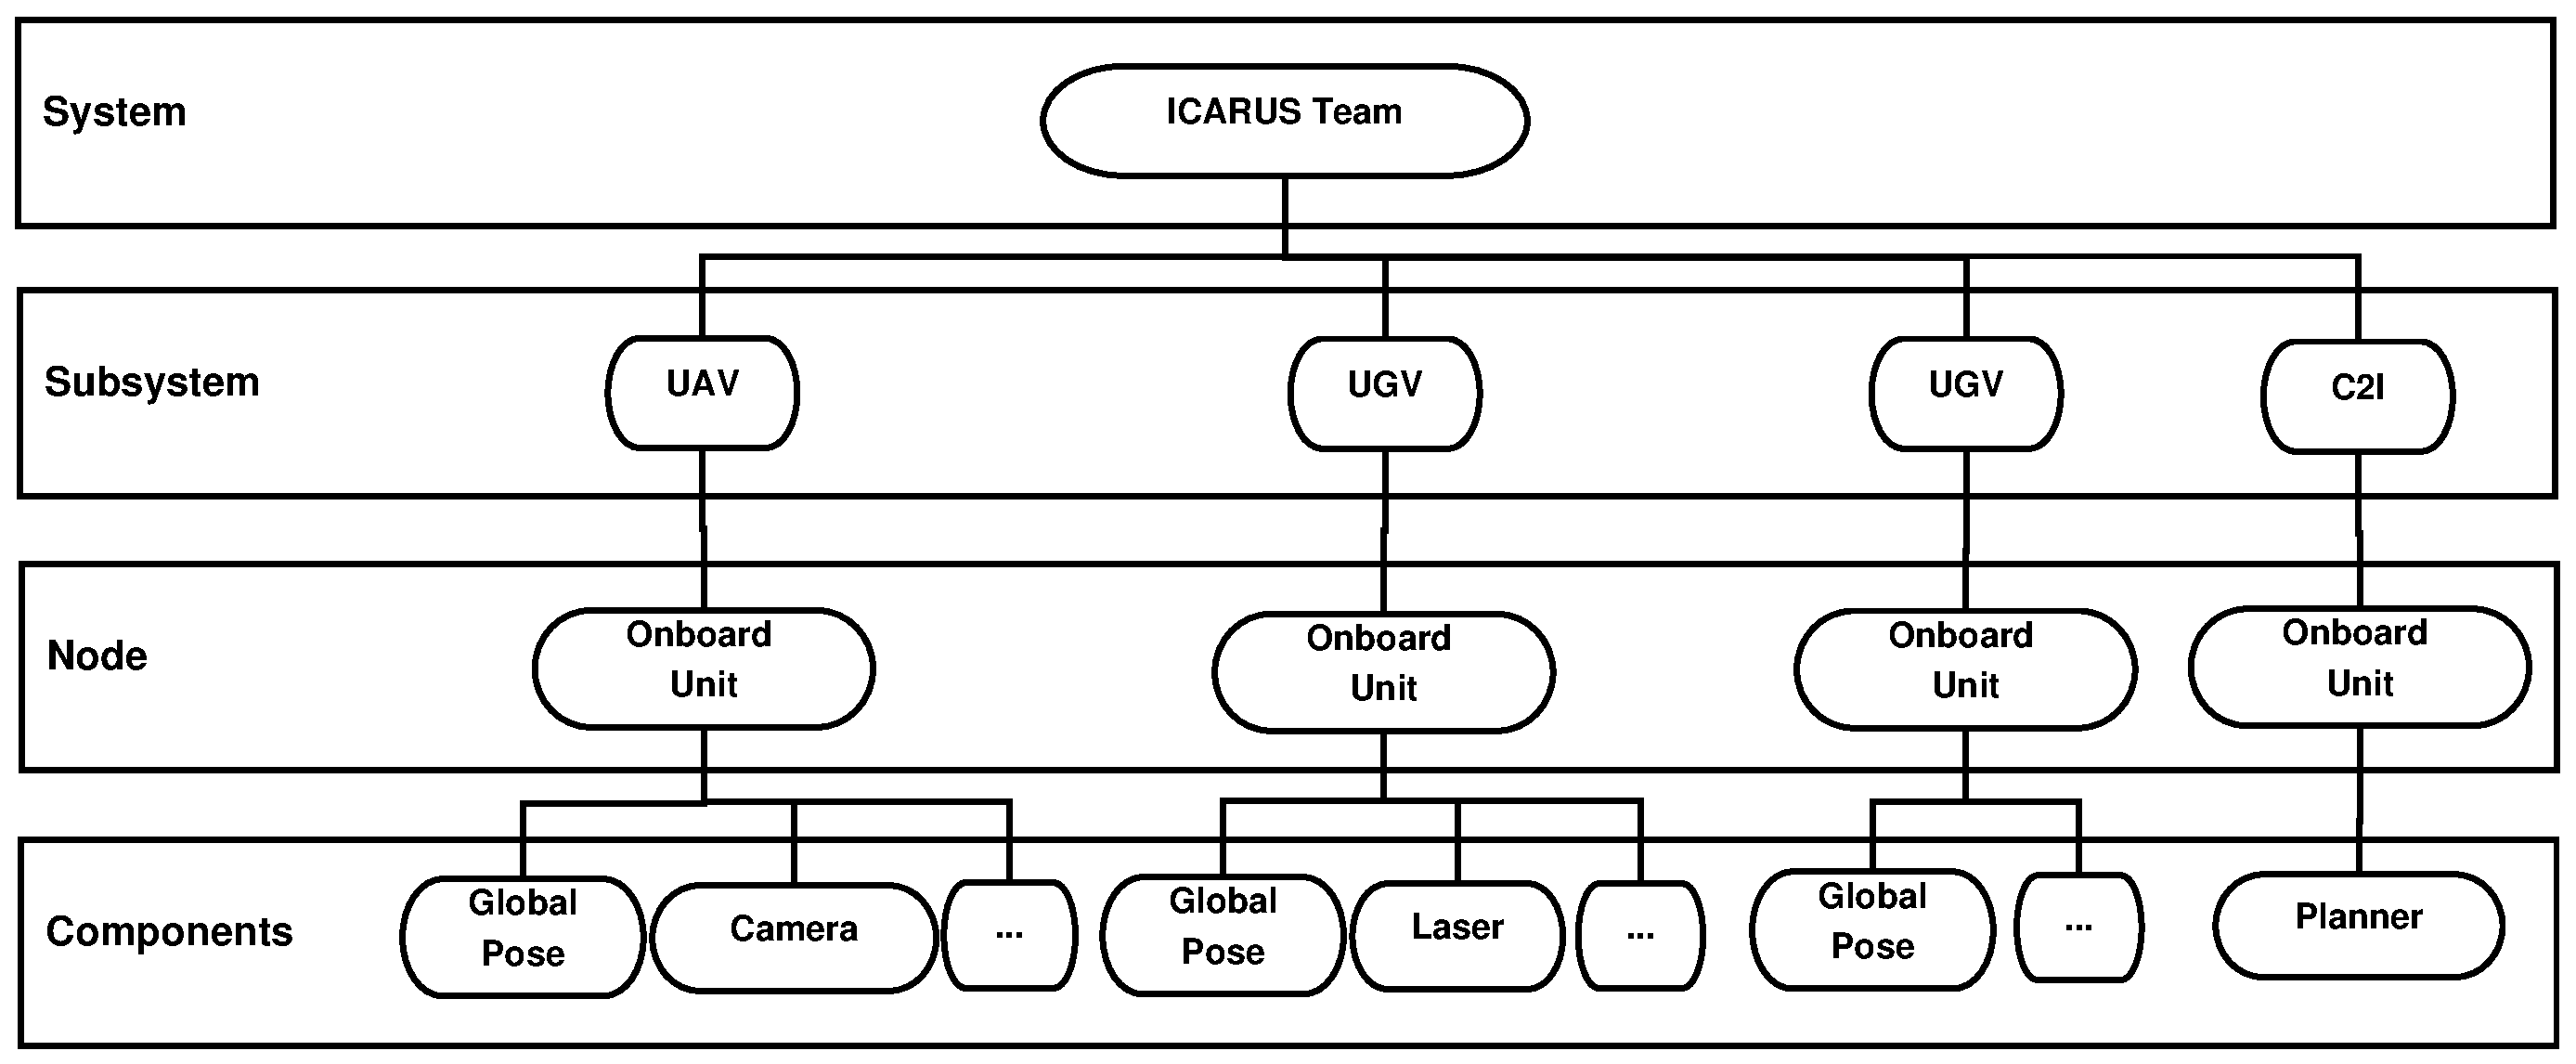
\includegraphics[trim=0cm 0cm 0cm 0cm, width=\textwidth]{ROB-15-0035_fig1.eps}
    \caption{A simplified example of ICARUS network topology.}
    \label{fig:icarus_topology}
\end{figure}

The work described in this paper has validated this approach in several realistic Search and Rescue missions, providing as well recommendations for extensions of the standard whenever a gap was identified, as for instance the need for an extended system status report including remaining autonomy, network quality, etc.

\subsection{Robot adaptation}
%\label{sec:adaptation}
The diagram in figure ~\ref{fig:robot_adaptation} illustrates different strategies for the integration of robots into the ICARUS team. Most robotics systems nowadays are based on existing proprietary or open-source middlewares such as ROS, MOOS, OROCOS, etc. To accommodate these systems into an ICARUS compliant network, the implementation of a software adapter or wrapper is required. This is illustrated by robots $A$ and $B$ in the diagram. This usually requires a preliminary analysis to identify equivalences between the standard JAUS services and the primitives in the platform-specific interfaces. This exercise usually requires a standardization step, removing any information that is specific to their particular implementations.

Robot $C$ instead depicts the native support. This strategy is only feasible when the standard interface is taken into account from the specification phase. In this case, the standard interface can also be used for inter-process communication within the system. This approach is usually more efficient since there is no translation step.

\begin{figure} [h!]
    \centering
    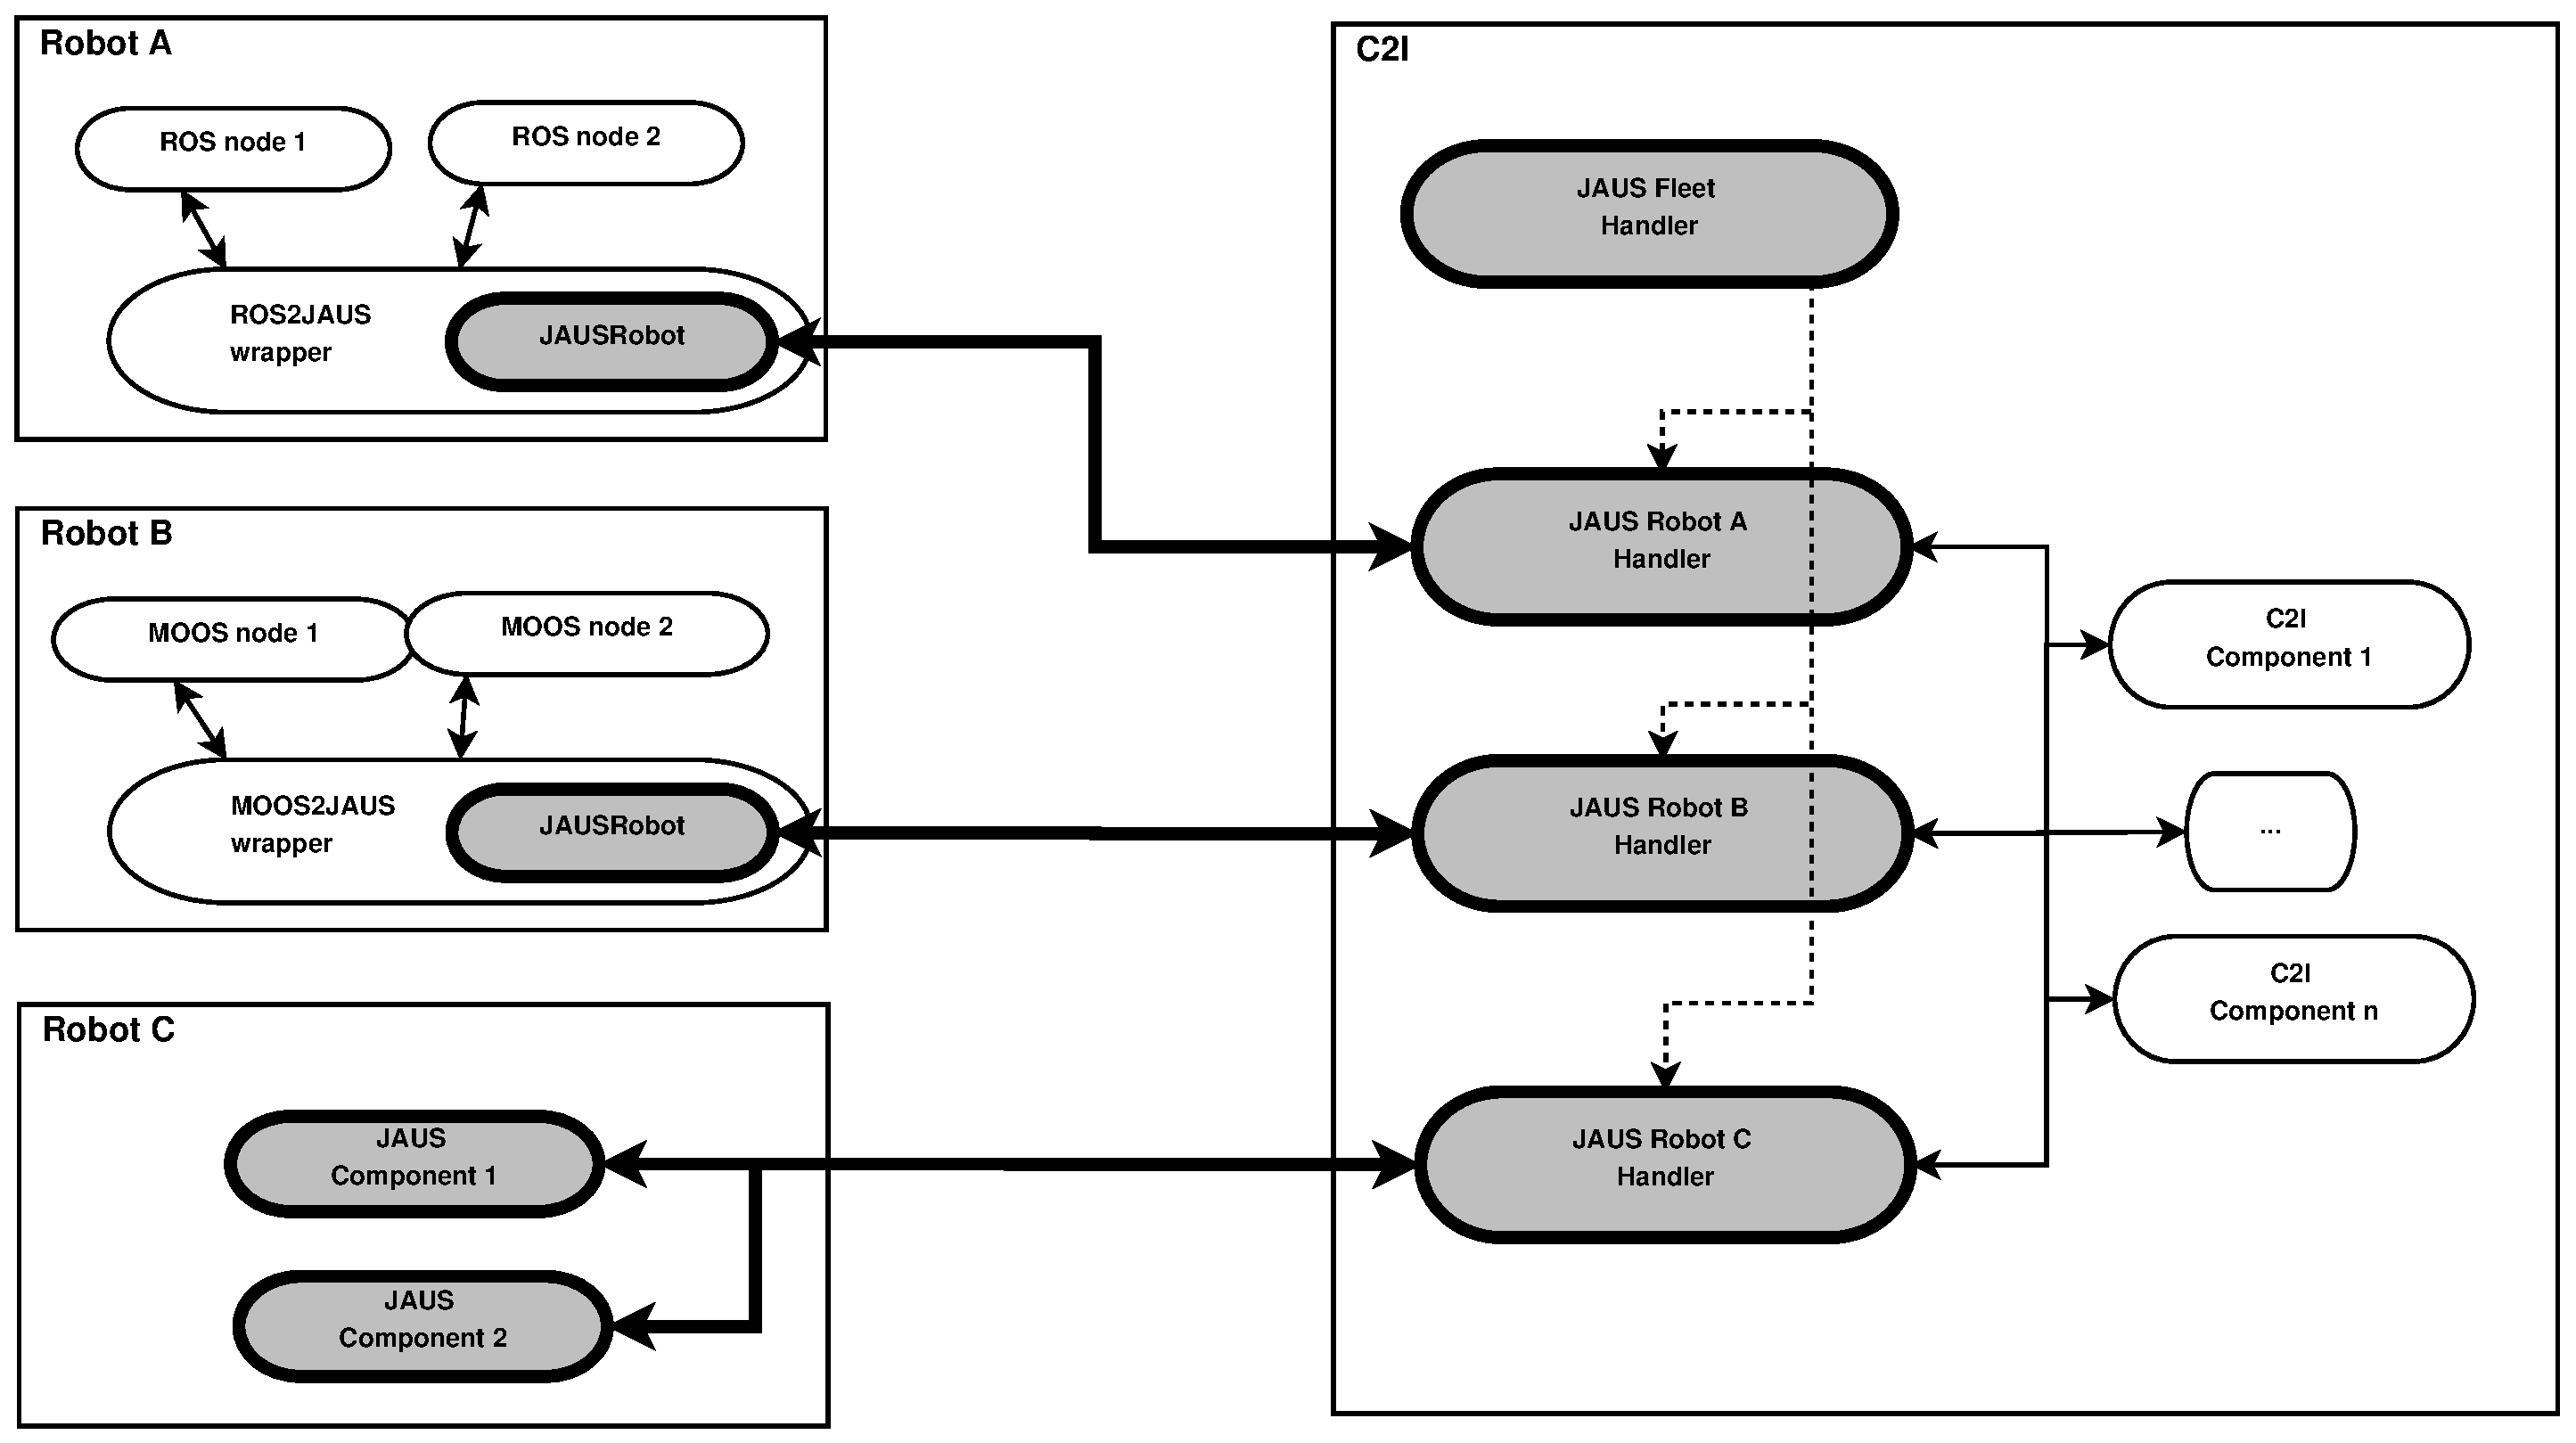
\includegraphics[trim=0cm 0cm 0cm 0cm, width=\textwidth]{ROB-15-0035_fig2.eps}
    \caption{Robots adaptation strategy.}
    \label{fig:robot_adaptation}
\end{figure}

All ICARUS platforms have been adapted to the ICARUS interface. This automatically ensures the compatibility with the ICARUS C2I, enabling the multi-robot coordination and combination of data as later described in this paper. The following tables describe the JAUS services used to carry out the experiments described in this paper:

\begin{table}[h!]
\centering
\begin{tabular}{| c | c | c |}
\hline
Sensor/Data Concept & Standard Service & Service Name \\
\hline
Pose Estimation        & Global Pose   & global pose    \\ \hline
VI sensor left camera  & Visual Sensor & left camera    \\ \hline
VI sensor right camera & Visual Sensor & right camera   \\ \hline
Stereo point cloud     & Range Sensor & point cloud     \\ \hline
FLIR Tau 2 640 		   & Visual Sensor & thermal camera \\ \hline
2D Laser Ranger		   & Range Sensor & 2D laser 	    \\ \hline
3D Laser Ranger		   & Range Sensor & 3D laser 	    \\ \hline
\end{tabular}
\caption{Standard Sensor Services}
\label{table:sensorservices}
\end{table}

\begin{table}[h!]
\centering
\begin{tabular}{| c | c | c |}
\hline
Driver Concept & Standard Service & Service Name \\ \hline
Remote Control          & Primitive Driver            & joystick control     \\ \hline
Waypoints 		        & Global Waypoint Driver      & global waypoint      \\ \hline
Paths	 		        & Global Waypoint List Driver & global waypoint list \\ \hline
\end{tabular}
\caption{Standard Driver Services}
\label{table:driverservices}
\end{table}

\subsection{Enabling robot collaboration}
The coordination of this team of robots in the field is a major challenge. An heterogeneous team usually contains a set of vehicles with very diverse capabilities. An effective heterogeneous team management requires reasoning about the mission goals based on the set of robot capabilities and constraints. To support these activities, some other aspects which are critical to ensure interoperability are the robust definition and specification of roles and tasks in the system, modes of operations and the adjustable level of automation.

The platforms involved in ICARUS have been carefully selected to complement each other. They can play different roles. Several ICARUS platforms form together a team, for each vehicle is specialized in one or more objectives but they also work together and support one another when executing more complex missions. Different strategies for the coordination are feasible. A strong end-users  \cite{b-fast}, requirement for the ICARUS project is the need for user authorization in any planning decision \footnote{Available on \url{www.fp7-icarus.eu/sites/fp7-icarus.eu/files/publications/D100-1 v8.0.pdf}}. Therefore, ICARUS follows a supervised loose coordination strategy where the interaction between robots is negotiated during mission planning. The planning, coordination and therefore the ultimate responsibility falls on the ICARUS Team Operator. To ensure optimal human-robots collaboration, these tools are seamlessly integrated into the C2I equipment of human crisis managers (see section \ref{command_and_control}) and a set of training and support tools is provided to learn to use the ICARUS system (see section \ref{training}).

A mission goal refers to the overall objective that the fleet must accomplish, in the case of the work presented in this paper is the assessment of a disaster area. The mission planning (see \ref{mission_planning}) is responsible to coordinate the fleet and to allocate equal or different roles to each of the robots. A role defines the robot's behaviour and its interactions with other members of the fleet or with humans. Typically, roles define which tasks a robot should and should not execute.

A robot is defined by the model or type of robot and its associated capabilities. These characteristics define the set of tasks that it is able to perform, and therefore, the set of roles it can take. One of the standard core services required to all the platforms is the discovery service. It allows the robots to advertise their capabilities over the network, enabling planning and supervision from the C2I based on the current state of the team. A robot may take different roles during a mission depending on the responsibilities that the C2I allocates to it.

A mission plan is therefore built upon the concepts of roles, tasks and responsibilities. The diagram in figure ~\ref{fig:goals_decomposition} illustrates how a mission is broken down into task in the ICARUS C2I.
\begin{figure} [h]
    \centering
    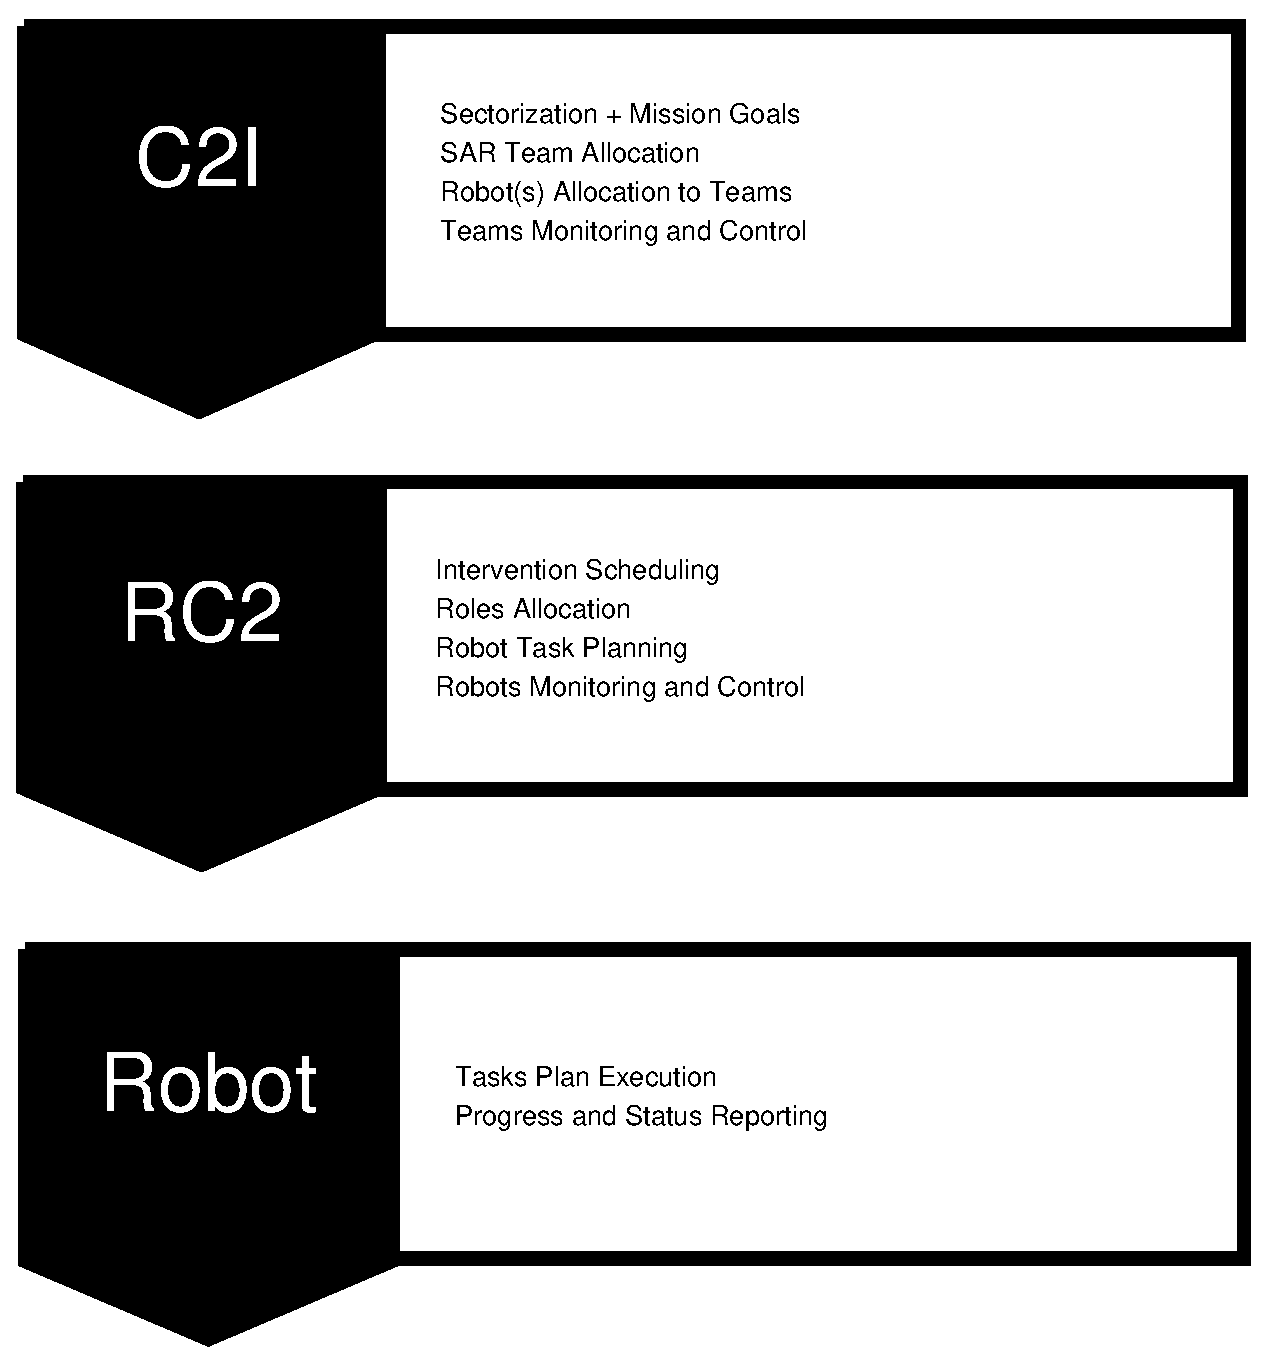
\includegraphics[trim=0cm 0cm 0cm 0cm,scale=0.5]{ROB-15-0035_fig3.eps}
    \caption{ICARUS Goals to Roles and Tasks decomposition}
    \label{fig:goals_decomposition}
\end{figure}
These are the different roles defined in the ICARUS concept of operations.
\begin{table}[h!]
\centering
\begin{tabular}{| l | p{5cm} | p{7cm} | }
\hline
Roles &	Description	& Modes \\ \hline
Scout &	Provides a quick assessment of an unexplored area or route. &
Overview of an entire disaster zone (Fixed-wing UAS).
Traversability/best route exploration (Fixed-wing UAS). \\ \hline
Surveyor &	Detailed scan of an area or building to support a thoroughly assessment and inspection (structure integrity, victims, hazards, etc). & 2D/3D geo-referenced “map” of the entire disaster zone as basis for sectorization (Fixed-wing UAS).
High resolution 2D/3D geo-referenced “map” of a sector (Fixed-wing UAS for higher altitude and Rotorcraft for lower altitude) or a structure (Rotorcraft).
Building indoors (autonomous) inspections (Small Rotorcraft and Small Unmanned Ground Vehicle(SUGV) ) \\ \hline
Observer &	Steady target (both victims and structures) observation and assessment. & •	Steady hover over a target (Rotorcraft), including harsh weather conditions. Victim medical state assessment outdoors (Rotorcraft), indoors (Small Rotorcraft) and both (SUGV). \\ \hline
Searcher &	Victims search. & Outdoors aerial long-range human detection on IR (Fixed-wing UAS). Outdoors aerial short-range detection on IR (Rotorcraft).Indoors short-range detection on IR (Rotorcraft). Indoors short-range detection on IR (SROT)
\\ \hline
Rescuer & Supports the rescue of victims & Helps victims to escape from hazard areas (SUGV) or supports human rescuers in their activities.  \\ \hline
Deliverer &	Safety kit delivery	& Delivery of a survival kit to a victim, aerial (Rotorcraft), terrestrial (SUGV) \\ \hline
Cruiser &	Travel to a destination.  & All platforms when transiting to a final destination where another role is enabled.
The larger platforms may also act as a Transporter carrying tools, debris or even the smaller platforms.\\ \hline
\end{tabular}
\caption{ICARUS robot roles}
\label{table:robotroles}
\end{table}
The allocation of mission goals to predefined roles, the decomposition of these roles into tasks, and the configuration of these tasks for a specific robot model, are responsibility of the mission planner. Some predefined profiles are available to facilitate this task.
Whereas roles influence the robots behaviour, tasks influence the actions that robots perform. They are defined as a set of actions. Each task could be decomposed into sub-tasks. This subdivision could continue iteratively until we reach a primitive task. The following tables lists a subset of ICARUS robot roles and tasks as an example:
\begin{table}[h!]
\centering
\begin{tabular}{| l | l | }
\hline
Category   & Tasks      \\ \hline
Operations & Launch	  \\ \hline
		   & Recovery \\ \hline
		   & Abort    \\ \hline
Mobility   & Set motion request \\ \hline
		   & Go to Waypoint     \\ \hline
		   & Standby            \\ \hline
		   & Return home        \\ \hline 	
  		   & Change Level of Automation \\ \hline 	
  		   & Mission management (start, stop, pause) \\ \hline 		
Advanced Mission Support & Scan 2D area  \\ \hline
		   & Scan 3D area                \\ \hline
		   & Search in area              \\ \hline
		   & Activate/Deactivate modules \\ \hline 	
  		   & Servoing around target      \\ \hline 	
Perception & Enable/Disable Payload      \\ \hline
		   & Capture payload             \\ \hline
		   & Configure payload           \\ \hline
Action/Grasping	Delivery & Robotic arm teleoperation \\ \hline  	
\end{tabular}
\caption{ICARUS robot tasks}
\label{table:robottasks}
\end{table}

\afterpage{\clearpage}

\section{A Data Management Architecture for Search and Rescue Robots}
High level mission planning, tracking and control is essential for deploying multiple Unmanned systems in reconnaissance and mapping tasks in a large and open environment.
Open-source and commercial ground control stations are available for controlling or planning the mission for single unmanned systems.
During our background research, open-source solutions were explored such as OpenPilot GCS\footnote{\url{www.openpilot.org/product/openpilot-gcs/}}, QGroundControl\footnote{\url{www.qgroundcontrol.org}} and happykillmore-gcs,\footnote{\url{https://code.google.com/p/happykillmore-gcs}} and commercial solutions such as UAV factory GCS\footnote{\url{www.uavfactory.com/product/16}} and  Alenia Aermacchi UAS GCS \cite{JIR_GCS}.
The availability of open source and field deployable multi-robot base control stations is not widespread, but limited to a few such as the multi-UAV QGroundControl, APM Planner, etc., to highlight a few.
Apart from allowing users to plan UAV missions, these utilities are not adapted to interface with ground or marine robots simultaneously.
Most openly available ground control systems are primarily designed to assist in the development and testing of unmanned systems while not targeted for search and rescue operations.
\subsection{Robot Command and Control Interface}
\subsubsection{Architecture}
The ICARUS-Command, Control and Intelligence (C2I) system represents a generic robot control base station capable of interfacing with unmanned systems deployed in controlled real-world SAR scenarios for mission planning, monitoring and execution.
In \cite{sgo-ssrr} we described the design concepts and capabilities of the C2I that were inspired by SAR first responders feedback from B-FAST (Belgian First Aid and Support Team).

The C2I system of ICARUS consists of a central Mission Planning and Coordination System (MPCS), portable Robot Command and Control (RC2) sub-systems and mobile devices.
The deployment of C2I sub-systems, with their communication links, for unmanned SAR operations is shown in Figure~\ref{fig:c2i_sys_arch}.
The C2I user interface design incorporated some of the human factors associated with Search and Rescue mission planning and monitoring with the use of ecological interface concepts \cite{EcoIf}.
\begin{figure}
    \centering
    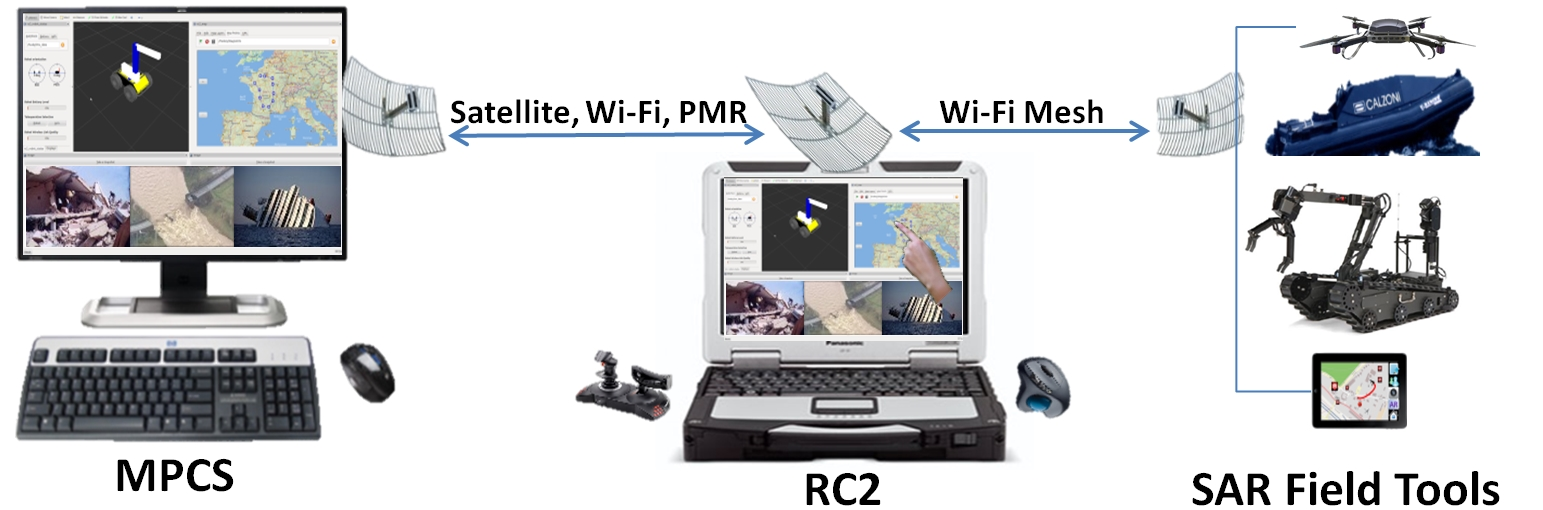
\includegraphics[width=\textwidth]{ROB-15-0035_fig4}
    \caption{C2I deployment and communication framework.}
    \label{fig:c2i_sys_arch}
\end{figure}
\begin{figure} [h]
    \centering
    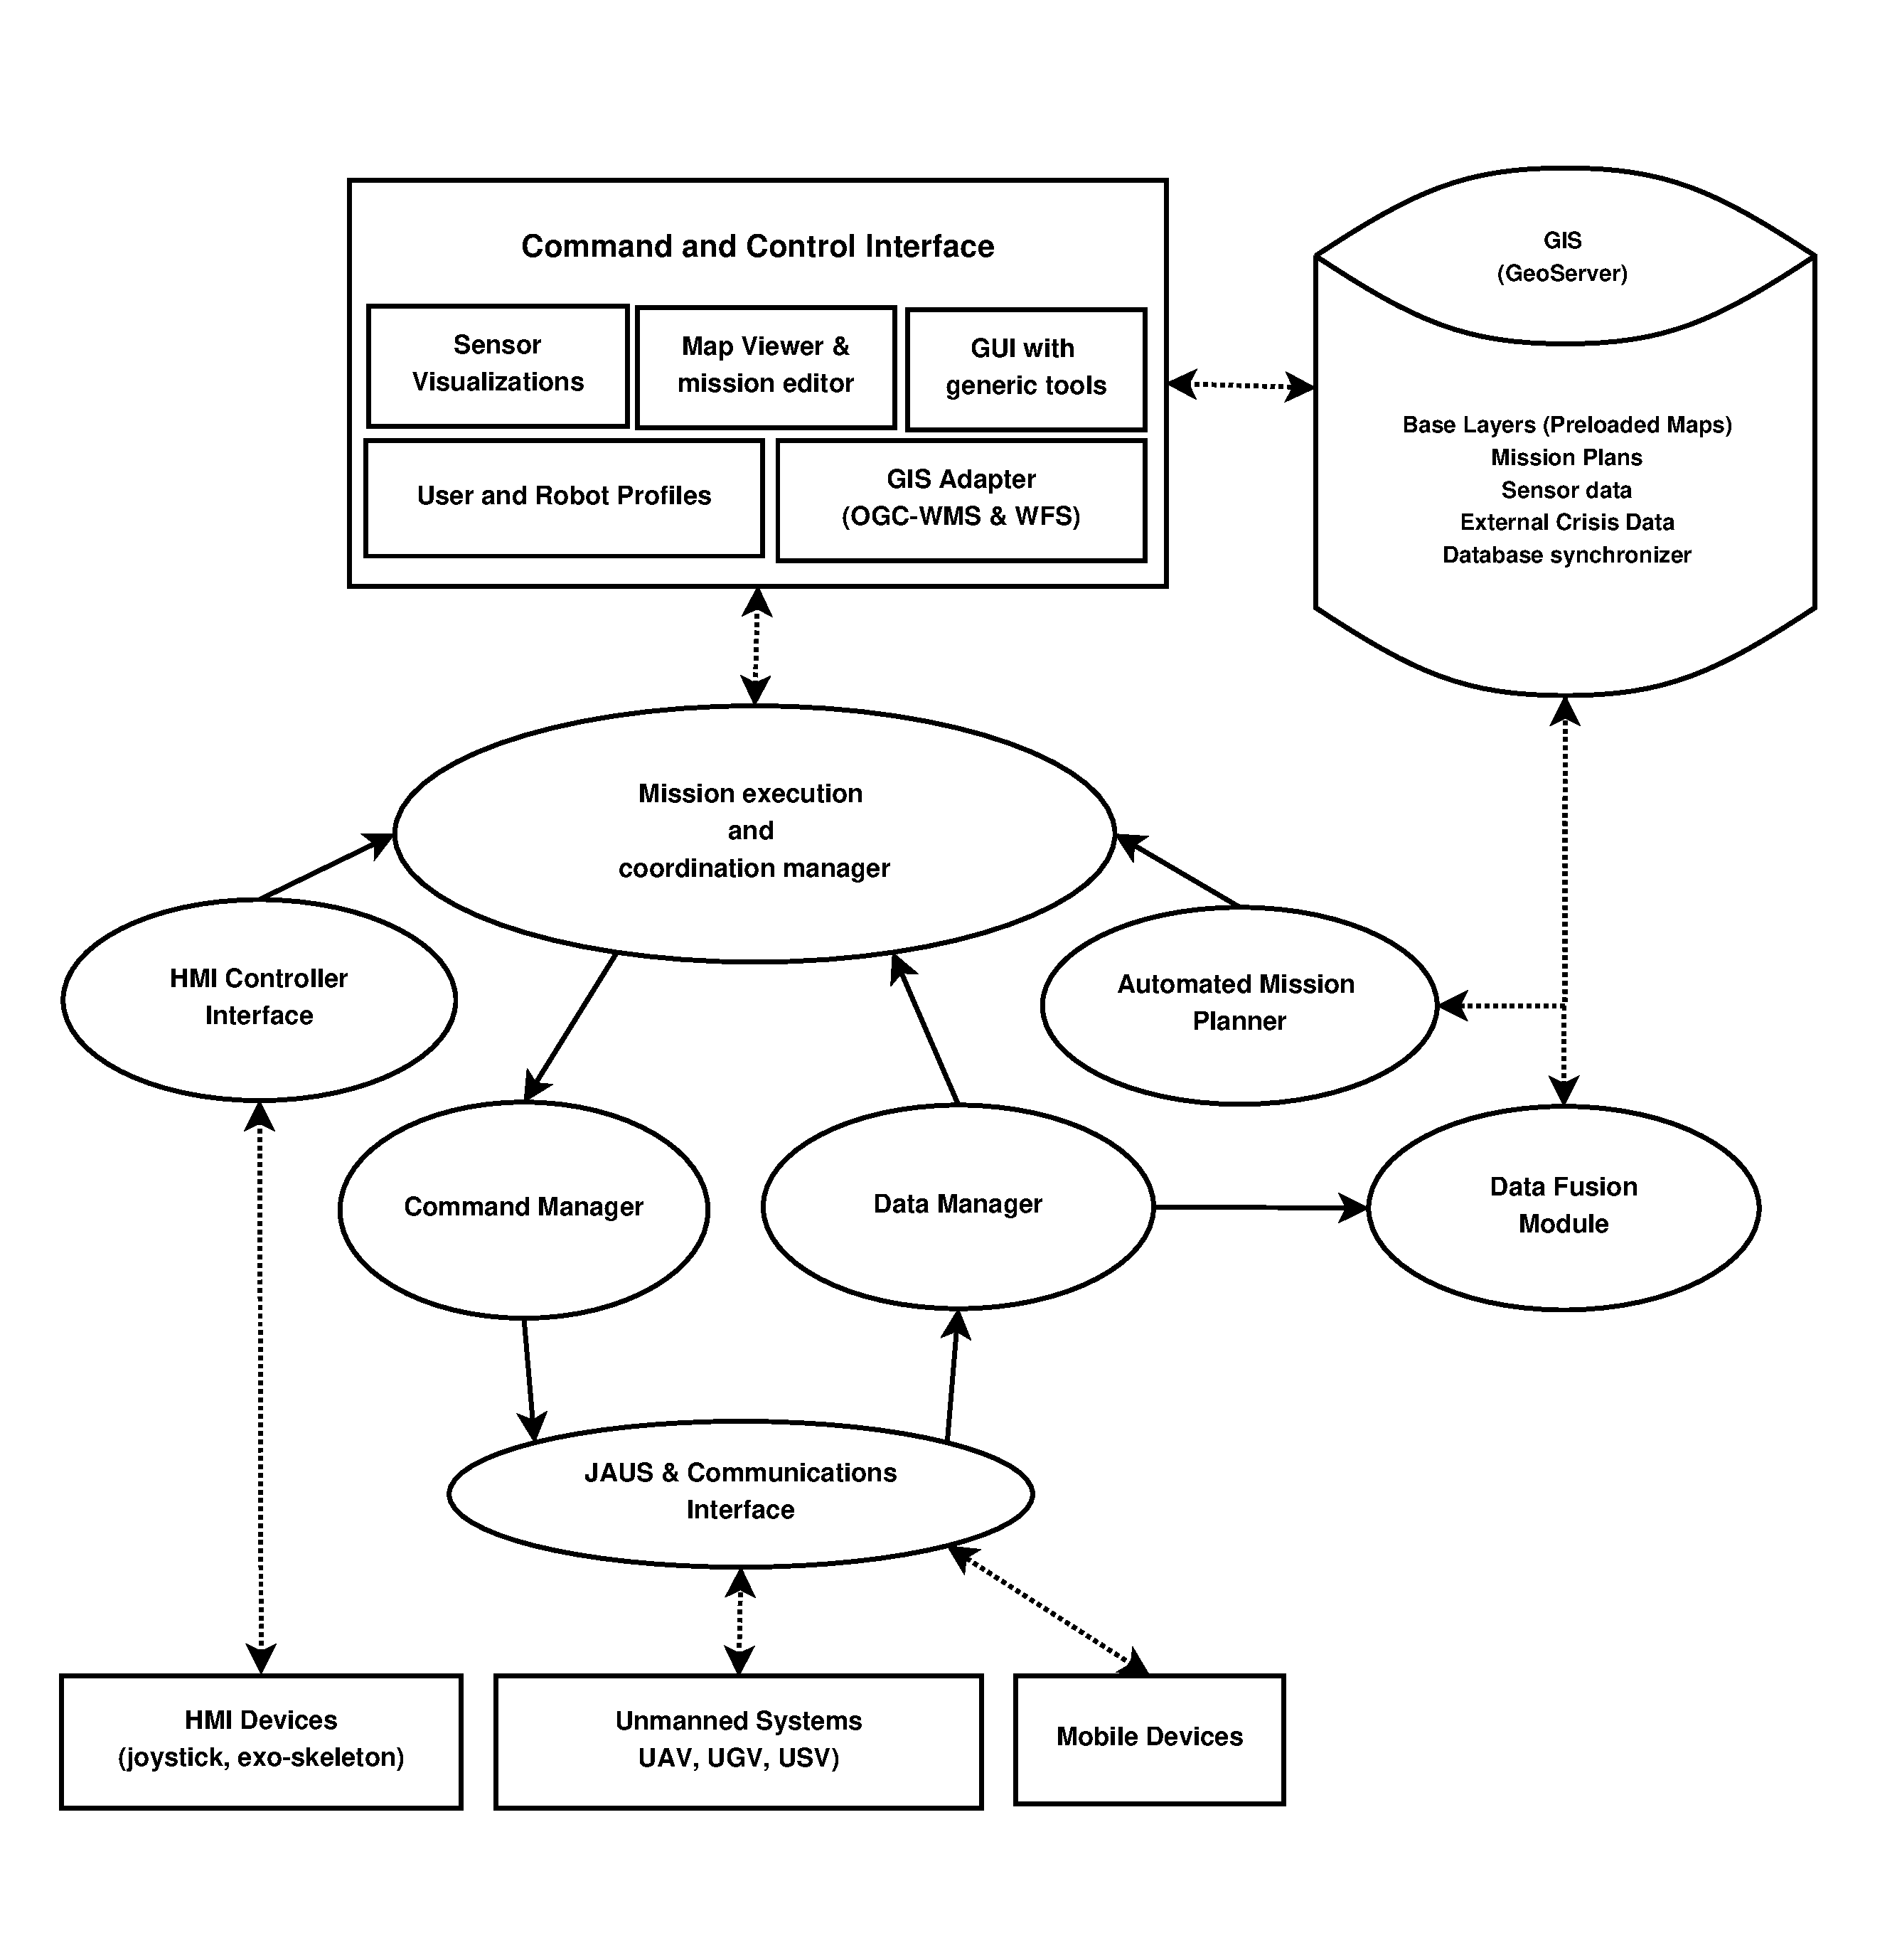
\includegraphics[width=0.85\textwidth]{ROB-15-0035_fig5.eps}
    \caption{C2I components (nodes) based on ROS.}
    \label{fig:c2i_ros_arch}
\end{figure}
The novelty of the C2I developed within the scope of search and rescue is based mainly on extensibility, standardization and interoperability.
The software architectures of the MPCS and RC2, shown in Figure~\ref{fig:c2i_ros_arch}, use the Robot Operating System (ROS) as their middleware.
The motivation behind the usage of a distributed framework like ROS is to maximize the reusability of available robot sensor visualizations, sensor fusion and control algorithms, and to adopt a standard framework used extensively on robotic platforms.
This approach is coherent for rapid integration of the C2I with diverse robotic platforms in different deployment scenarios and provides a flexible approach in comparison with contemporary solutions.
Most existing commercial robot command and control centers are either coupled to a specific robot platform or to a specific SAR deployment scenario.
Currently the C2I is scalable and can support multiple unmanned platforms and dynamic addition or removal of a robot within the ICARUS network.
The ROS-JAUS bridge (as explained in section 2.2) has enabled the C2I to be interfaced with robots and simulators implementing either ROS or JAUS interfaces.
The JAUS fleet handler informs the C2I at runtime regarding addition or removal of robot within the network and updates on state of existing robot services.
This event triggers the C2I to configure sensor visualization widgets, map elements, trigger actions and tools for each robot dynamically, requiring no user interaction for managing settings for each robot.
Robots are currently connected to the base station over multiple WiFi links.
Work on selectively adding higher fidelity and long range communication links such as satellite and Private Mobile Radio (PMR) to both the ground station and unmanned systems are ongoing.
\subsubsection{GIS sensor data management}
Open Geospatial Consortium (OGC) standards have been used for storing and retrieving raster and vectorial data from the Geographic Information System (GIS) Geoserver.
The embedded C2I map client was developed using OpenLayers SDK to produce a homogeneous web client capable of being rendered on standard browsers running on PC's and mobile platforms.
The map client uses OGC Web Map Service (WMS) to access raster maps and render multiple layers.
The Web Feature Service (WFS) has been extensively utilized by the map client to access and render vectorial map data from Open Street Maps (OSM), elevation contour maps, points of interest for SAR etc.
The GIS database is also configured to store temporal geotagged sensor data from multiple robots such as global pose, trajectories, waypoints, sectors, victim positions, images, videos, point clouds along with their respective map styling information.
WFS-transaction (WFS-t) operations are triggered from the map client and the C2I back end framework to insert or update data incoming from unmanned systems.
Different sensor observations are depicted as layers within the map viewer where each sensor observation is linked to a geometry (point, line or polygon) on the map with an appropriate icon.
External crisis data providers such as Global Disaster Alert and Coordination System (GDACS\footnote{\url{ www.gdacs.org}}) and MapAction\footnote{\url{ www.mapaction.org}} are among the most widely used sources providing rapid updates regarding worldwide crises, associated maps from field personnel and RSS data feeds.
A service has been developed to parse RSS feeds and extract information, maps, images and online links to be stored into an adapted database in the GIS.
This information is rendered within the map client (Figure~\ref{fig:c2i_ortho_UAVs}) as a layer with current and historical data, accessed by custom popups based on the information to be displayed on the map.
\subsubsection{Mission planning and operations control}
\begin{figure} [h]
    \centering
    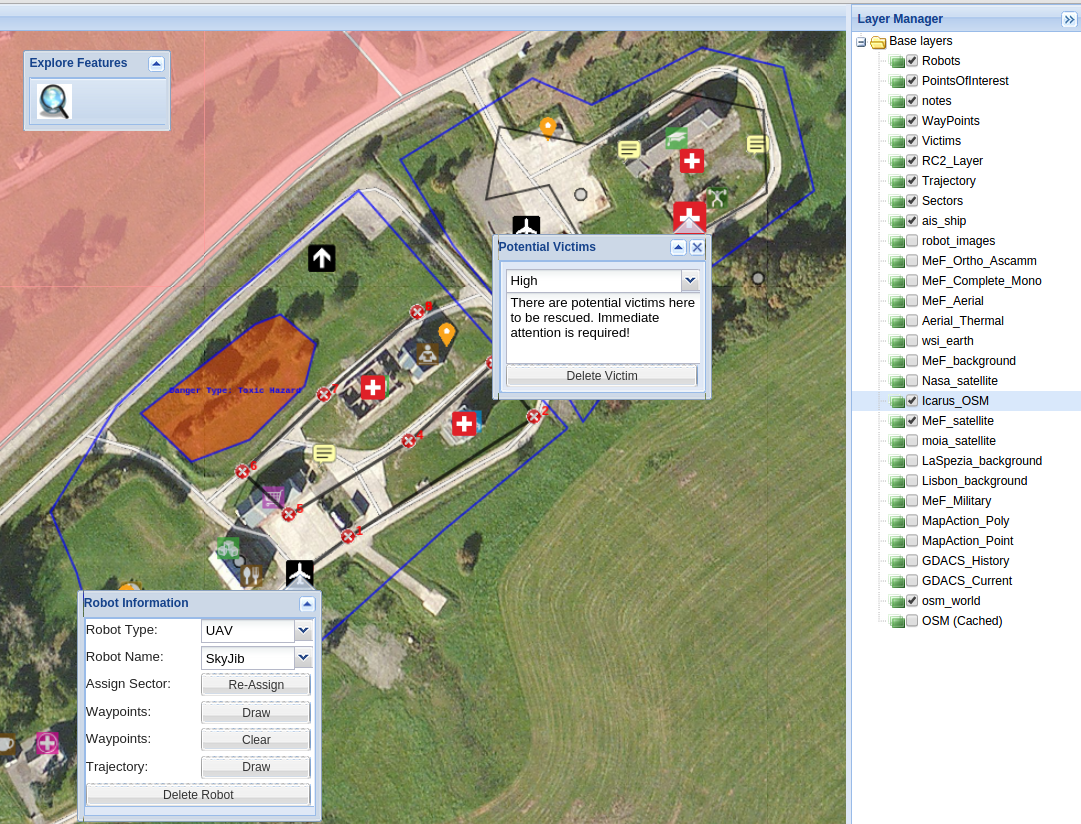
\includegraphics[width=\textwidth]{ROB-15-0035_fig6.png}
    \caption{C2I: Mission Planning and Coordination System (MPCS).}
    \label{fig:c2i_mpcs_viz}
\end{figure}
Figure ~\ref{fig:c2i_mpcs_viz} and ~\ref{fig:c2i_rc2_viz} provide a generic overview of the C2I graphical user interface.
SAR first responders perform mission planning over base map views which include Google base and satellite maps in the presence of a satellite or mobile internet link in the area of operations.
The SAR community operates in disaster stricken areas with limited or no network availability.
To remain operational in a real deployment scenario, the C2I hosts a local Geographic Information System (GIS) server with Open Street Maps (OSM) vectorial data such as roads, buildings, water bodies etc. with relevant styling, aerial maps from UAV's as GeoTiff overlays, vectorial and raster maps obtained from civilian or military authorities, enabling the C2I to provide consistent base maps for mission planning.
Rasters downloaded from Google and Bing maps can also be added to the GIS layers for offline access, but this requires a commercial license, which is beyond the scope of our current C2I requirements.
Mission planning begins with the central SAR operations manager to sectorize an area into zones of operations. SAR resources including unmanned platforms and human SAR personnel are assigned to each sector based on the area under coverage, complexity of the environment and operations. The MPCS operator can draw points of interest, add notes, mark potential areas with victims and hazardous zones over existing base maps. The operator can also author high level waypoints or reference trajectories with associated metadata for each robot on the map for describing desired exploration and surveillance tasks.

\begin{figure} [h]
    \centering
    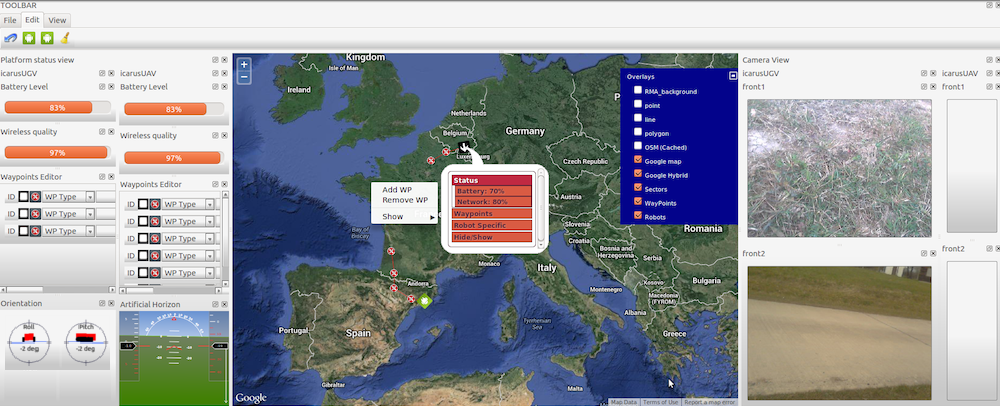
\includegraphics[width=\textwidth]{ROB-15-0035_fig7.png}
    \caption{C2I: Sensor visualization in RC2 during SAR operations.}
    \label{fig:c2i_rc2_viz}
\end{figure}

The Robot Command and Control Station (RC2) receives a reference SAR mission plan from the MPCS through the GIS. Local planning for robots involves the operator referring to the mission plan and authoring a detailed set of waypoints on the base map with associated metadata for describing desired goals.
The waypoint editor facilitates the user to set parameters specific to a robot depending on its level of supported autonomy.
Default or specific values can be set for each waypoint such as altitudes (for UAV's), waypoint tolerance and path tolerance radius.
Temporal data can be associated with many actions such as starting or take-off position, final or landing position, pass through point, loiter position with altitude or radius, desired robot heading and velocity and point to focus or track with the camera.
Robots connected to the RC2 have individual sets of sensor data rendering widgets displaying information such as location (GPS) and global orientation on the map, inertial measurements (roll \& pitch) for UGV’s and integrated artificial horizon for UAV’s, multiple video camera streams (raw or compressed), battery level and wireless link quality indicators, waypoints list editor and an optional point cloud (raw or processed 3D maps) rendering widget. The left side of Figure ~\ref{fig:c2i_rc2_viz} shows the sensor visualizations widgets customized for each type of robot based on its application for land, air or marine scenarios. For example, aerial robots have an artificial horizon widget displaying inertial sensor information (attitude, rate of ascent) while ground robots have a graphical representation of roll and pitch angles. Global orientation of each platform is represented on the map layer within the robot icon.

\subsection{Data Fusion}
\subsubsection{Related Work}
Mapping of unstructured environments in 2D and 3D is currently a popular research topic. Research is being carried on finding sensor systems for the task \cite{sensor2} and mapping strategies and algorithms \cite{method1}.
Even different means of unusual sensor transportation, such as using canines are being tested \cite{canine}.
The visualization of gathered data is also a problem that was analyzed from many different angles.
The 2D representations of unstructured environments tend to be occupancy maps \cite{ocmap1}\cite{ocmap2}, because of their usefulness for planning and low memory consumption.
In paper \cite{RIM} the authors use Rich Information Maps for environment representation.
This approach fusses a Kinect 3D map with object and human recognition and tracking to present a fuller representation of the environment. In \cite{isosurface} a polygon mesh representation, created using isosurfaces of a coarse 3D occupancy grid is presented.
Another approach is using voxels for environment representation \cite{voxels1}.
Finally, work is being carried in the area of using augmented reality for visualization to better integrate the operator into the robot's decision making \cite{AugmMap1}.


In our approach, we concentrate on merging 3D point clouds using a  modified ICP algorithm (base method introduced in \cite{baseICP}).
For visualization, we use direct point clouds rendering with a customizable point size.
This approach has the merit of representing accurately real-life environmental data with minimal deformation from computation.
The drawback is the high computational load of such a rendering and the difficulty of interpretation for human users.
We minimize those problems by using semantic classification of individual points and using GRID servers for computation purposes.
\subsubsection{Processing Pipeline}
This section describes the proposed 6D-SLAM algorithm. Figure ~\ref{fig:6DSLAM} shows the scheme of the algorithm.
Green rectangles correspond to novel algorithmic components using high performance computing in CUDA (Compute Unified Device Architecture): filtering and subsampling, semantic classification and semantic 3D scan matching.
The semantic approach efficiently decreases the time of the 6D-SLAM convergence, by requiring a lower number of iterations, especially in the situation where odometry readings are not sufficiently accurate.
It is also more reliable than state of the art approaches for demanding scenarios, such as moving down stairs or mapping harsh environments.
In the following subsections, the main components of the algorithm will be described.
\begin{figure}
    \centering
    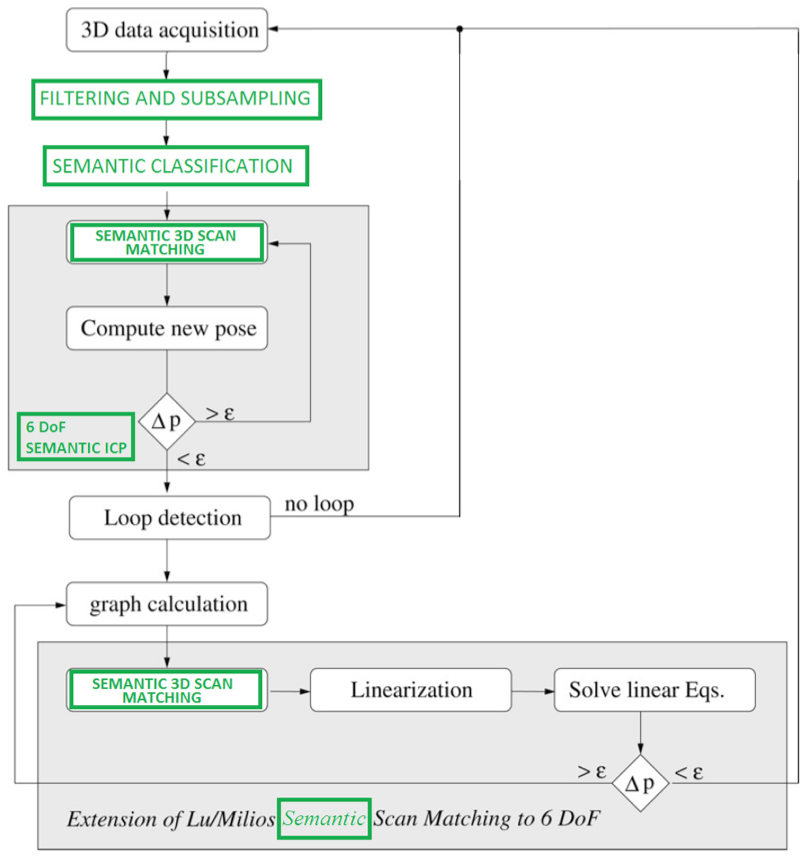
\includegraphics[height=4.0in]{ROB-15-0035_fig8.png}
    \caption{6D-SLAM Processing Pipeline Scheme.}
    \label{fig:6DSLAM}
\end{figure}
\subsubsection{Filtering and subsampling}
This algorithmic component prepares the 3D data for further analysis.
For efficient NNS (Nearest Neighbourhood Search), a regular grid decomposition (RGD) strategy is used, as explained in our previous work ~\cite{Bedkowski2012}.
The implementation allows to perform calculations for each 3D point in parallel.
%RGD decomposes 3D space into 64, 128, 256 or 512 buckets for each direction.
RGD strategy decomposes the 3D space of the point cloud into a set of buckets. The decomposition may be done in two ways: having a set number of buckets in each direction (64, 128, 256 or 512) or by using a constant size of the bucket (1x1x1m etc.).
The first strategy is better suited for the filtering stage, while the second one is useful during subsampling.
During the filtering phase for each query point, 27 surrounding buckets are searched to find the nearest neighbours.
If the number of neighbours for given points is lower than a threshold it is removed from the data set (see algorithm \ref{algorithm:filtering}).
Filtering is used to remove, from the point cloud, points that are most likely a measurement error and should not influence future calculations.
	The subsampling is done to achieve a common density between different point clouds.
This is required because the scanning technique used on UGV's tends to gather clouds whose density changes with range.
The second problem is the density difference between aerial point clouds and ground point clouds. Subsampling itself is a simple process.
After decomposing the point cloud into buckets of given size, from each bucket a single point, closest to the centroid, is left while others are erased.
By changing the size of the bucket different densities can by achieved.
Figure \ref{fig:sparseresults} shows an example of a subsampling result while Algorithm ~\ref{algorithm:sparse} shows the procedure.
\begin{algorithm}
\caption{3D data filtering}
\begin{algorithmic}
\label{algorithm:filtering}
\STATE INPUT: Point cloud M=$\{m_{xyz}\}$
\STATE OUTPUT: Filtered point cloud M
\FOR{all points $m_{xyz}$ in parallel}
  \STATE find $bucket_m$
  \STATE update \textit{table\_of\_found\_buckets}
\ENDFOR
\STATE in parallel sort \textit{table\_of\_found\_buckets} \COMMENT{radix sort}
\STATE in parallel count points in each bucket
\FOR{all query points in parallel}
  \STATE find bucket
  \FOR{all neighboring buckets}
    \STATE count amount of NN{ }for{ }query points
  \ENDFOR
  \STATE mark to erase if count $<$ threshold
\ENDFOR
\STATE erase all marked points
\end{algorithmic}
\end{algorithm}
\begin{algorithm}
\caption{3D Data sub-sampling}
\begin{algorithmic}
\label{algorithm:sparse}
\STATE INPUT: Point cloud M=$\{m_{xyz}\}$
\STATE OUTPUT: Point cloud N with decreased, uniformed density
\FOR{all points $m_{xyz}$ in parallel}
  \STATE find $bucket_m$
  \STATE update \textit{table\_of\_found\_buckets}
\ENDFOR
\STATE in parallel sort \textit{table\_of\_found\_buckets} \COMMENT{radix sort}
\STATE in parallel count points in each bucket
\STATE in parallel compute centroids for all buckets
\FOR{all buckets}
 \FOR{all points in current bucket}
  \STATE find distance from centroid
 \ENDFOR
 \STATE mark point with minimal distance to the centroid
\ENDFOR
\STATE copy marked points as a result
\end{algorithmic}
\end{algorithm}
\begin{figure} [h]
    \centering
    \begin{subfigure} [br]{0.45\textwidth}
         \centering
         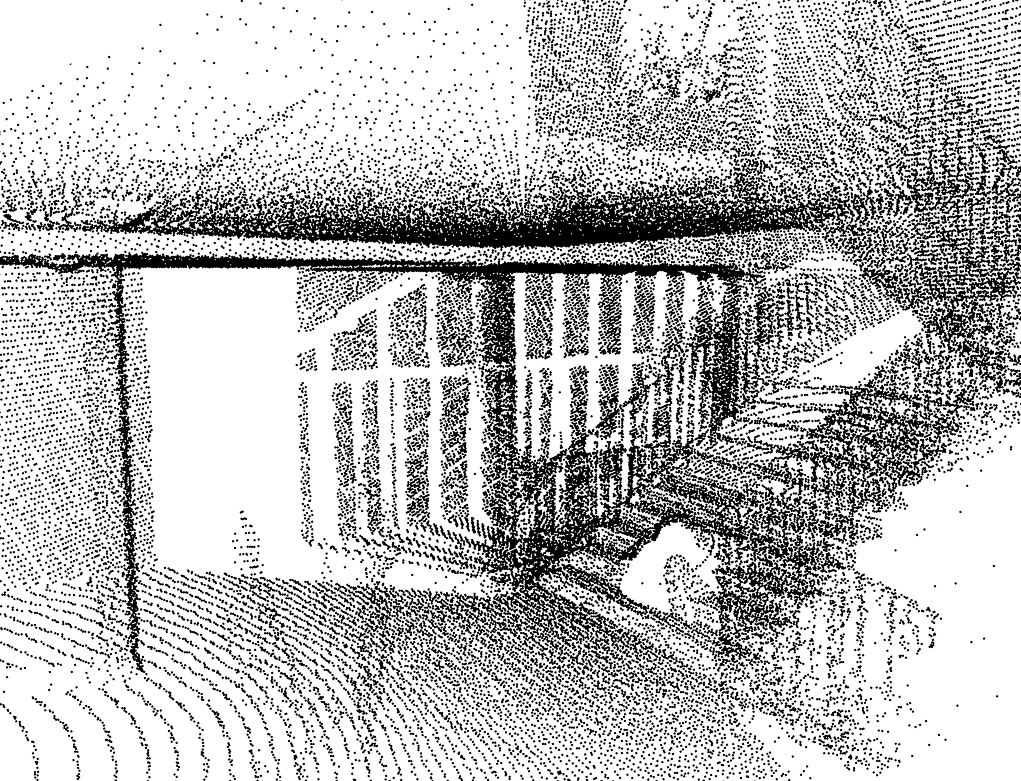
\includegraphics[width=\textwidth]{ROB-15-0035_fig9a.png}
         \caption{Initial point cloud}
         %\label{fig:drrobot}
    \end{subfigure}
    \begin{subfigure} [bl]{0.45\textwidth}
         \centering
         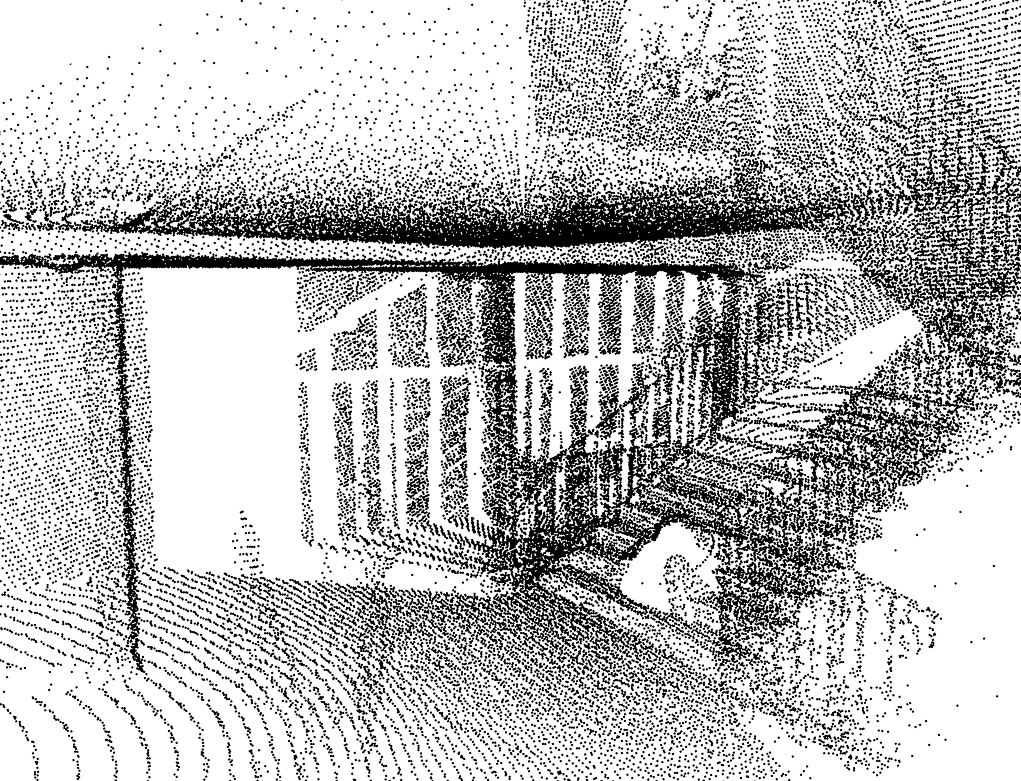
\includegraphics[width=\textwidth]{ROB-15-0035_fig9a.png}
         \caption{Subsampled point cloud.}
         %\label{fig:husky}
    \end{subfigure}
    \caption{Subsampling example using 7.3 mln points; the resulting point cloud has ~400.000 points.}
    \label{fig:sparseresults}
\end{figure}

\subsubsection{Semantic classification}
Semantic classification assigns class (wall, ceiling, floor, edge) label to each query point.
The procedure is executed in parallel.
Classification helps in the scan matching process.
The first step of classification is normal vector estimation based on PCA (Principal Component Analysis) using SVD (Singular Value Decomposition) method, as described in our previous work devoted to General Purpose Computing on Graphics Processing Units (GPGPU) for robotic applications ~\cite{nuechter2013e}.
A point with a normal vector can be treated as a plane.
In the second phase each point is assigned an initial class: flat or edge.
The classification is done based on the analysis of the neighbourhood (for example all points in a 25cm radius) for each point.
If the majority of points in the neighbourhood is closer to the plane described by the given point, the point is classified as flat, otherwise it is classified as an edge.
The third phase differentiates between floors, ceilings and walls.
Flat points that are below the center of scan and whose normal vectors are pointing up are considered floor.
Flat points that are above the center of the scan with normal vectors pointing down are considered ceiling. Finally flat points whose normal vectors are roughly horizontal are considered walls.

The classification procedure helps in points' discrimination in the consecutive ICP (Iterative Closest Point) procedure and in the NNS for loop closing.
The classification algorithm is aimed mainly for ground robots, as they are more likely to work in an environment where ceiling and floor are visible.
This simple procedure is works also in outdoor environments as it is able to detect planes under and above the robot.
Nevertheless the second phase's flat/non-flat classification may be done for aerial point clouds. It is important to emphasize that, from matching the point of view, it is more important that the classification is consistent between different point clouds than the human semantic correctness of classification itself.
As shown in the results section 6, the presented approach gave good results in unstructured SAR-like environments.

\subsubsection{Semantic scan matching}
The main part of scan matching algorithm is a modified ICP algorithm.
Our improvements concentrate on a parallel computing implementation and discriminating points into four classes during the nearest neighborhood search procedure.
The key concept of the ICP algorithm can be summarized in two steps ~\cite{Segal-RSS-09}:
\begin{enumerate}
\item Compute correspondences between the two scans (Nearest Neighbour Search),
\item Compute a transformation which minimizes distance between corresponding points.
\end{enumerate}
Iteratively repeating these two steps results in convergence to the desired transformation.
Semantic discrimination of these correspondences improves the convergence.
Range images (scans) are defined as model set $M$ where
\begin{equation}
|M|=N_m
\end{equation}
and data set $D$ where
\begin{equation}
|D|=N_d
\end{equation}
The goal of semantic ICP is to minimize following cost function:
\begin{equation}
\label{equation:errorfunc}
E\left ( \mathbf{R,t} \right )=\sum_{i=1}^{N_m}\sum_{j=1}^{N_d}w_{ij}\left \| \mathbf{m}_i^c-\left ( \mathbf{Rd}_j^c+\mathbf{t} \right ) \right \|^{2}
\end{equation}
where $w_{ij}$ is assigned 1 if the $i^{th}$ point of $M$ correspond to the $j^{th}$ point in $D$ in the sense of minimum distance and the same class.
Otherwise $w_{ij}$=0.
Class $c$ discriminates points into wall, ceiling, floor or edge.
{\bf R} is the rotation matrix, {\bf t} is the translation matrix, {\bf m}$_i^c$ corresponds to points of class c from the model set $M$, {\bf d}$_j^c$ corresponds to points of class $c$ from the data set $D$.
The algorithmic representation of the process is shown in algorithm ~\ref{algorithm:gpgpuICPsemantic}.

\begin{algorithm}
\caption{Semantic ICP - parallel computing approach}
\begin{algorithmic}
\label{algorithm:gpgpuICPsemantic}
\STATE INPUT: Two point clouds M = $\{m_i\}$, D= $\{d_i\}$, an initial transformation $T_0$, semantic label for each point $\{wall, edge, ceiling, floor, stairs...\}$
\STATE OUTPUT: The transformation T, which aligns M and D
\STATE $M_{device} \leftarrow M $
\STATE $D_{device} \leftarrow D $
\STATE $T_{device} \leftarrow{T_0}$

\FOR{$iter \leftarrow 0$ to $maxIterations$}
    \FOR{$i \leftarrow 0$ to $N$ \COMMENT {in parallel}}
        \STATE $m_{i}^{c}\leftarrow$ FindClosestPointAssumingTheSameClass($T_{device}\cdot d_{i}^{c}$)
    \IF {found $m_{i}^{c}$}
        \STATE $w_{i}\leftarrow 1$
    \ELSE
	\STATE $w_{i}\leftarrow 0$
    \ENDIF
  \ENDFOR
  \STATE $T_{device} \leftarrow \underset{T_{device}}{argmin} \left \{ \sum_{i}^{} w_{i} \left \| T\cdot d_{i}^{c}-m_{i}^{c}  \right \| ^{2}  \right \}  $ \COMMENT {calculation T$\leftarrow$ R,t with SVD}
\ENDFOR
\STATE $M \leftarrow M_{device} $
\STATE $D \leftarrow D_{device} $
\STATE $T \leftarrow T_{device} $
\end{algorithmic}
\end{algorithm}

\subsubsection{6DSLAM}
The core of our 6DSLAM contribution was inspired by the work ~\cite{Borrmann:2008:GCM:1342428.1342686}.
To improve the accuracy and reliability of the scan matching we add semantic discrimination of points what was also done in ~\cite{Nuchter053dmapping} and ~\cite{Pfaff:2007:EEE:1229565.1229570}.
The main difference of our approach with respect to the state of the art is a novel semantic classification and usage of a parallel programming model for improving the performance of computation.
Another advantage of the approach is that all needed computation can be performed in a cloud, capable of virtualizing GPUs (NVIDIA GRID technology).
The cloud system provides means to perform 3D mapping based on many sources (mobile robots equipped with 3D lasers) in parallel and then to merge all maps into a common coordinate system.
In this paper, we demonstrate the 3D map building done by our cloud system, based on data from two independent UGVs and one UAV.
The 3D map can be distributed in the cloud in a SaaS (Software as a Service) model.
As a result, many end users can have immediate access to the results of the robots' perceptual survey.

\subsection{Comparison with State of the Art}
For the comparison purposes, we implemented an open-source SLAM algorithm on top of PCL (Point Cloud Library, GitHub, \url{https://github.com/LIDER-MSAS/data_registration_pcl} ) and a standard dataset for the robotics community (\url{http://lider.zms.imm.org.pl/downloads}). We performed an experiment on the well-known data set $hannover2$ (3DTK framework, http://slam6d.sourceforge.net). Figure \ref{fig:comparison} demonstrates five trajectories, allowing us to compare the PCL-based data registration (trajectory PCL\_ICP) with our semantic approach (semantic\_icp). Three of the trajectories show 3 step of presented processing pipeline: scan matching with semantic\_icp (semantic\_icp.xml), loop closing with ELCH (Explicit Loop Closing Heuristic) with CSH (Complex Shape Histogram)\cite{CSH_DARPA} used for detecting the loop (elch\_csh.xml), Lu/Milios style relaxation in postproccesing  (lum.xml). Semantic ICP shows a major improvement of data registration accuracy in comparison to PCL ICP, thus it can be concluded that semantic classification can be considered as an added value.

An additional observation is that loop closing procedures do not provide a major improvement int comparison with the one obtained with semantic ICP. Thus, we claim that the semantic registration gives accurate and reliable mapping that is already useful for end users.

\begin{figure} [h]
            \centering
         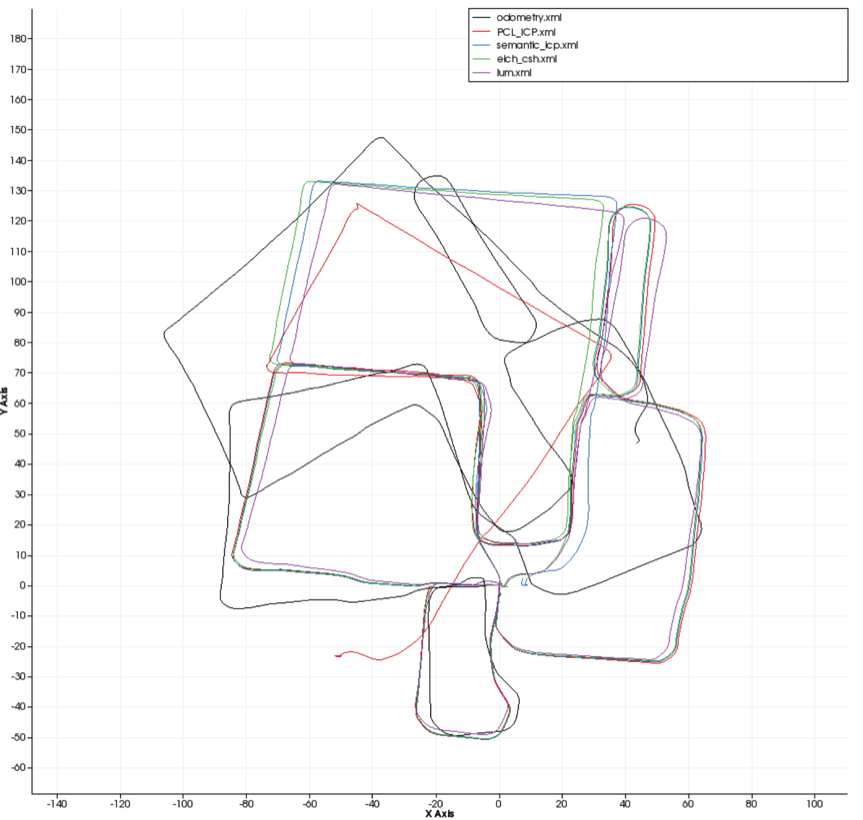
\includegraphics[width=\textwidth]{ROB-15-0035_fig10.png}
         \caption{Comparison of trajectories obtained with different approaches: raw odometry (odometry.xml), open-source PCL implementation of ICP (PCL\_ICP.xml), presented semantic implementation of ICP (semantic\_icp.xml), semantic ICP with ELCH (elch\_csh.xml), semantic ICP with ELCH and LUM postprocessing (lum.xml).}
         \label{fig:comparison}
   \end{figure}

\afterpage{\clearpage}


\section{High Performance Computing (HPC) in the Cloud for data fusion} 


High Performance Computing in the Cloud is relatively new topic especially in mobile robotics. One of the problems of mobile platforms is the availability of computation solutions that have good power to energy consumption ratio. This limitation is extremely visible in hte area of parallel computing, as most graphic cards' energy requirements are challenging for small platforms.
Since NVIDIA launched the Jetson TK1 micro supercomputer, it is possible to run CUDA programs on a low-energy (5 Watt) machine with 192 CUDA cores.
There still exists a problem of availability of higher computation power for more demanding operations, especially in the field.
We decided to provide computation power through a mobile data center based on an NVIDIA GRID server (Supermicro RZ-1240i-NVK2 with two VGXK2 cards - in total 4 GPUs with 4GB RAM each) capable of GPU virtualization.
This Mobile Data Centre, which is a server inside ruggedized chassis, is shown on figure ~\ref{fig:grid}.

\begin{figure} [h]
            \centering
         \includegraphics[width=\textwidth]{ROB-15-0035_fig11.png}
         \caption{Novel mobile data centre for SAR missions - ruggedized NVIDIA GRID.}
         \label{fig:grid}
   \end{figure}

To simplify interactions with the server, we deployed a Citrix framework. Citrix allows creating virtual systems for a number of users and gives access to them through a thin client, available from the server through a web browser. The main advantage of this approach is that all computation takes place on the server, while the user experience is similar to working with a local machine. Citrix can be deployed in two architectures:  VDI (Virtual Desktop Infrastructure) and XenApp, both of which have been used in our server.
In a VDI model, each GPU can be used by up to 8 users having access to virtual machine.
In XenApp, many users can share a single GPU by giving access to a Windows Server system or published applications.
VDI basically gives the user an access to a fully virtual workstation that can be accessed from any computer with Citrix receiver thin-client.
The drawback of this approach is the reservation of hardware. The hardware  to the virtual machine is constant and can not be changed dynamically, even when user is currently not using the full capacity. Change of assigned hardware is possible only after virtual system shutdown. 

Another problem is lack of CUDA support if more than one user is using a single GPU.
XenApp dose not have those problems, as it gives the user access to chosen applications and assigns the computation power according to local needs.
The drawback is lack of access to applications not foreseen by the system administrator.
For the computation pipeline shown in this article we decided to use the XenApp model, because it allows to share the hardware resources, especially CUDA, between users.
This approach seems sensible as the number of applications needed is limited and there exists no need for quickly changing them.
These applications can be accessed in SaaS model from a web browser after installing a thin client, which is a Citrix Receiver working on any operating system on any device.
The GRID technology supports building applications with sophisticated rendering (OpenGL 4.4) and CUDA.
Thus, it is used for registering and rendering the 3D cloud of points for SAR missions and also for building training tools. 
The software in the data center is compatible with data formats of Icarus platforms.
The system is scalable and can perform mapping for multiple robots (UAVs + UGVs).
To provide the CLOUD-like operation of the ruggedized server, it is equipped with a 5GHz WiFi router for creating a local network.
The users may connect to the network and get access to the computation power of the server through their own personal devices.
The results of one user work are available to other users, which makes the cooperation easier.
This also means that the data have to be uploaded to the server only once.

As such, it may be stated that the server deploys a local cloud for data processing management and distribution.
If the server is connected to the Internet, it can then work as a global cloud and stream the maps to any other users connected to the Internet (the data can be shown for example to an expert in another country).
It is important to emphasize that by using Citrix technology the bandwidth required to work with the data is minimal, as only the compressed renders are sent over the network.

\afterpage{\clearpage}

\section{Virtual Training via the C2I Interface}\label{training}
Search and Rescue operations demand rapid response requiring extensive SAR personnel training before deployment.
Previous and ongoing research projects NIfTi \cite{NIFTI}, ICARUS ~\cite{ICARUS}, SHERPA \cite{sherpa}, DARIUS \cite{darius}, VIEW-FINDER\cite{viewfinder}, GUARDIANS\cite{guardians} aimed at introducing unmanned systems into existing SAR infrastructure have shown that extensive end user training is essential for effective operation during deployment of diverse and complex robotic platforms.
However, SAR personnel in general may not be well acquainted with robot capabilities and interfaces due to limited access to unmanned systems and relevant resources.
Simulators capable of representing interactions between unmanned platforms within disaster scenarios with high fidelity can supplement hands on training.
A number of training simulators for robotic platforms are available today:
\begin{itemize}
  \item The simulation tool USARsim ~\cite{Carpin2007}  (Unified System for Automation and Robot Simulation) is a high fidelity simulator for Urban Search and Rescue (USAR) robots. It is dedicated to the research activities and concentrates on the human-robot interaction and the coordination of multiple mobile platforms. USARsim provides access to the diverse environments such as highway’s, DARPA urban challenge arenas, robotic soccer, etc., and different models such as the submarines, humanoids or helicopters. One of the simulator’s test environments is based on National Institute of Standards' (NIST) Reference Test Facility for Autonomous Mobile Robots for Urban Search and Rescue.
  \item ARGoS is a simulator for multi-robot interaction (http://iridia.ulb.ac.be/argos/home.php) released under GPLv3.0.
ARGoS is a state-of-the-art, open source robot simulator. Its main design focus is the simulation of large heterogeneous swarms of robots, therefore a robot team can be simulated simultaneously.
The main features of ARGoS are: its modular architecture (robots, devices, physics engines, visualizations and controllers are all handled as plugins), its multi-threaded architecture, its capability to run multiple physics engines simultaneously and its capability to tune the accuracy of every aspect of the simulation.
  \item Gazebo is a multi robot simulation environment, mainly aimed for use in robotics.
The features include: large database of robotic platforms and sensors, four high performance physics engines (ODE, Bullet, Simbody, DART) and high quality visualization using OGRE.
Gazebo's potential uses include algorithm testing and robot design.
  \item V-REP is a cross-platform multi robot simulator, free for educational use. It supports multiple physics engines and allows for collision simulation, dynamic particle simulation, inverse/forward kinematic calculation, etc.
Among other features there are rapid simulation scene modification, a rich database of platforms and sensors and an SDK for seven programming languages.
  \item Morse is a generic simulator for academic robotics.
The main aim is the simulation of various environments for multiple autonomous platforms.
Morse has a database of sensors, actuators and robotic platforms ready to use.
An interesting feature is the ability to customize how realistic different components of the simulation are. Because of that, the user may adjust the simulation to his needs, while maintaining real-time performance.
\end{itemize}
However, the mentioned solutions do not guarantee a high enough level of fidelity and dynamic simulation.
The physics layers of most mentioned simulators are so-called game engines that do not focus heavily on the fidelity of simulation.
A very important part of training in the area of SAR is to recreate real conditions as well as possible.
As it is nearly impossible to fully simulate a disaster zone, we have made a decision to concentrate on accurate simulated robot behavior to increase the usefulness of the virtual training.
Consequently, we have decided to develop a dedicated simulation framework based on the VORTEX physics engine.
Vortex is a closed-source, commercial physics engine for high fidelity dynamic simulation.
Its features include:
\begin{itemize}
\item Realistic parameter mapping - Vortex allows for setting the true parameters of objects and achieve realistic behavior, while other physics engines often require unrealistic values (much lower mass etc.),
\item Joint and gripping simulation - Vortex manages to significantly reduce the anomalies in the gripping process and joint interaction,
\item Fast and accurate collision detection.
\end{itemize}
%For our system we have developed a dedicated simulation framework based on VORTEX physics engine, which%
Apart from simulation engine itself, Vortex comes with a set of tools for fast model creation.
The model behaviour can be customized through python scripts.
This functionality is very useful for our application as many of the ICARUS components are custom made and are unavailable in  common databases.


The framework adds value by closing the loop between training and deployment by linking a standard C2I interface for real and virtual robot control.
The advantage of this approach is the full integration of the simulation with the robots' controls. Additionally, the data gathered by the SAR systems may be used for creating realistic training environments.

The ICARUS interface is based on the Joint Architecture for Unmanned Systems (JAUS).
The integration approach into our ROS-based system is shown in Figure~\ref{fig:c2i_robot_sim_interface}.
\begin{figure} [h]
    \centering
    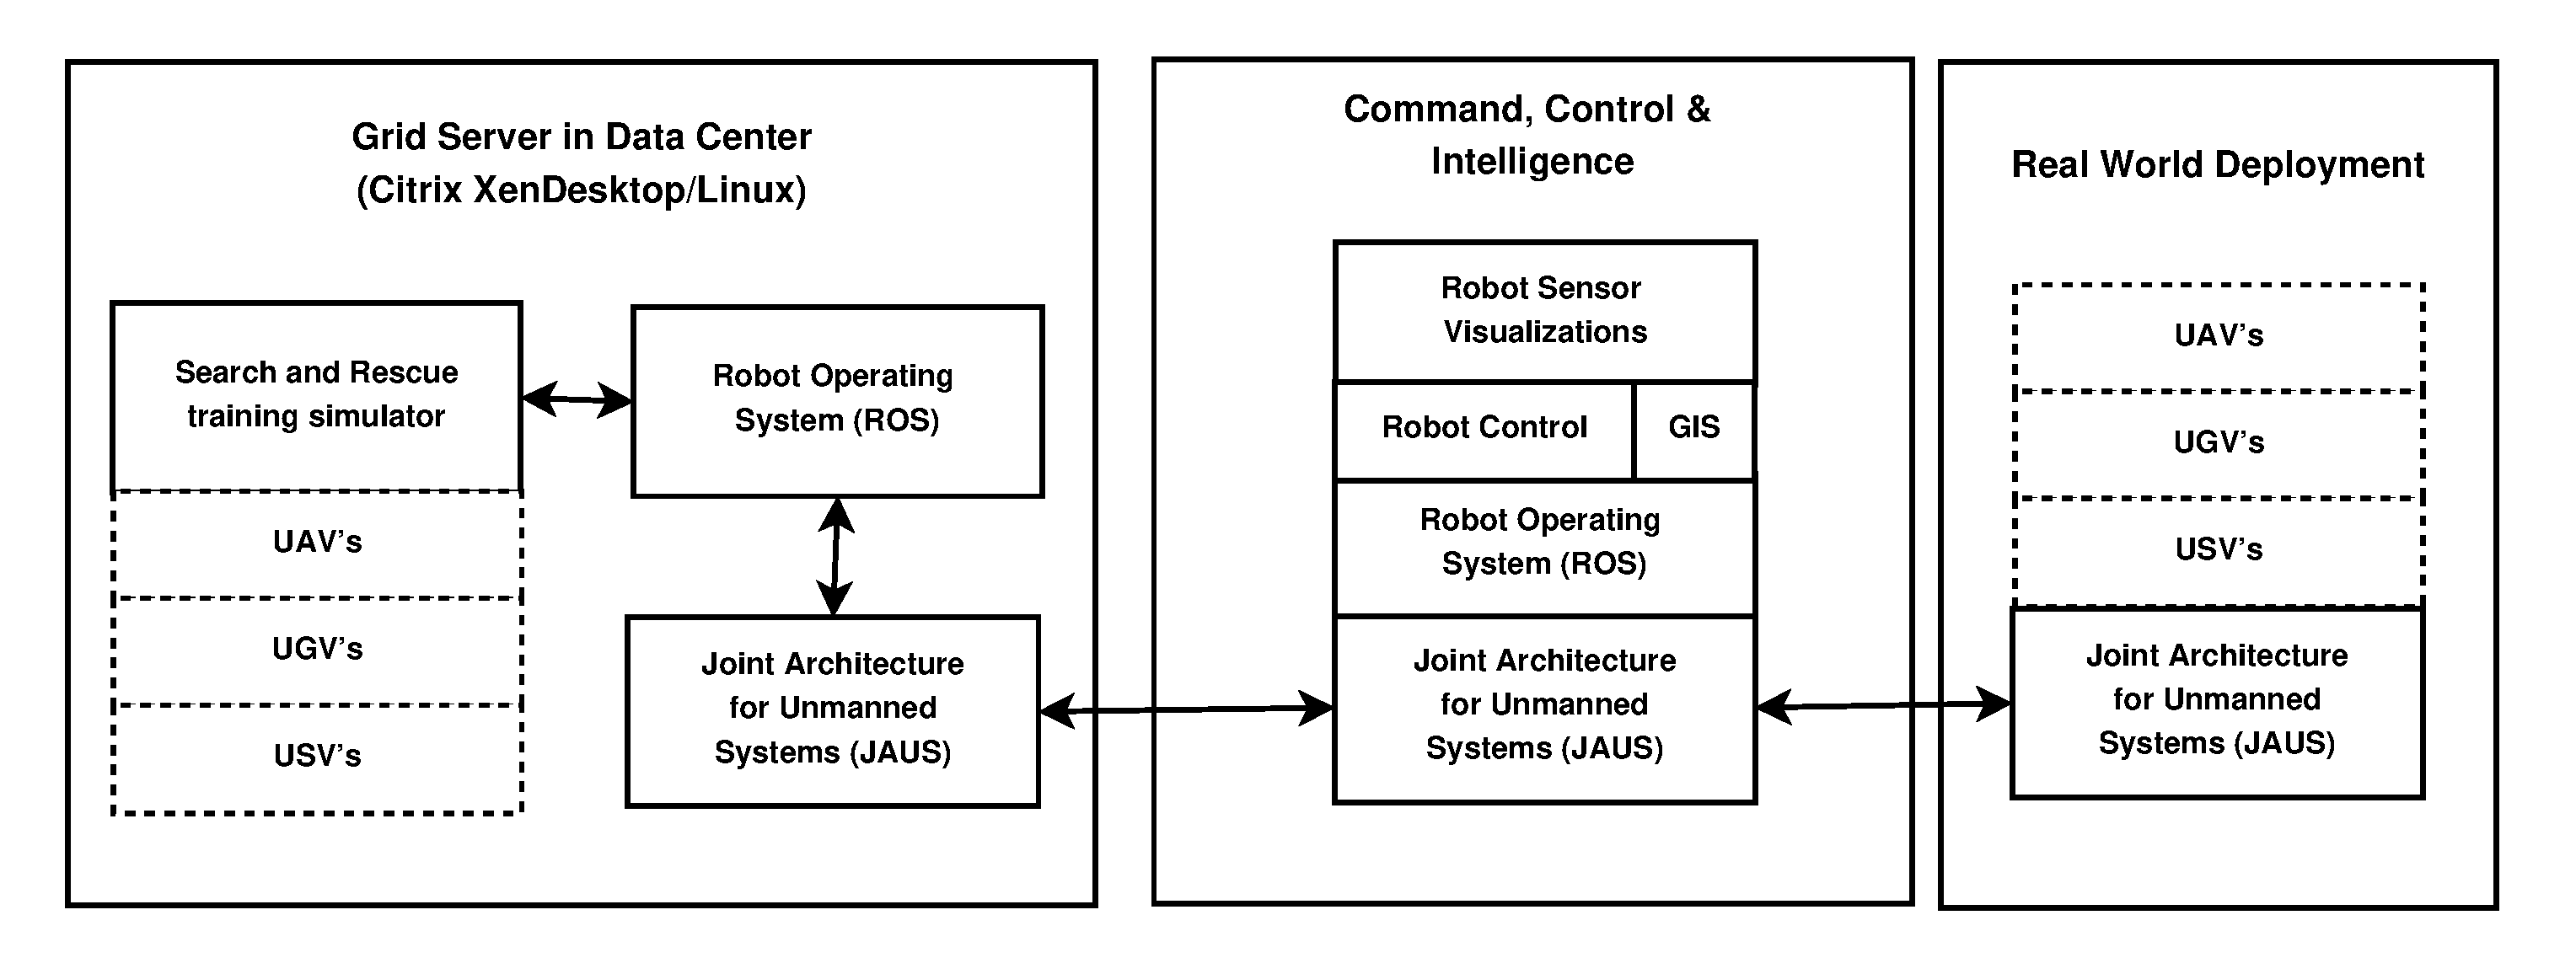
\includegraphics[width=\textwidth]{ROB-15-0035_fig12.eps}
    \caption{C2I interface between robots and simulator.}
    \label{fig:c2i_robot_sim_interface}
\end{figure}
The sequence of events for closed loop support between controlling robots in the real world versus the virtual environment is shown in Figure~\ref{fig:c2i_real_virtual_flow}.
SAR field response involves the deployment of platforms controlled from the C2I to execute a mission. Mission and sensor data are stored in the C2I GIS.
After the mission is completed, imagery and point cloud data captured by ground and aerial platforms are converted to ROS bags and passed to the data fusion module.
Accurately registered colored point cloud data and stitched aerial imagery generated by the fusion module are pushed to the C2I GIS and to the SAR training simulator.
The C2I simultaneously renders the fused point cloud data in a widget along with the aerial ortho-mosaic as a georeferenced layer overlaid on the base map.
Virtual sensor data from robots such as the global pose, inertial measurements and cameras are rendered within the C2I while controlling the UGV and its slave robot arm in the simulator through a joystick.
The slave robot arm was used to manipulate objects within the simulated environment for clearing rubble.

The simulator uses the fused 3D maps as a basis to create a virtual environment populated with UGVs and UAVs. Semantic classification is performed for the map. After this step, the following elements are automatically extracted:
\begin{itemize}
\item Digital Terrain Model (DTM) - created based on the ground points
\item Locations and bounding boxes of objects
\item Rough triangle meshes for ray-tracing (Sensor simulation)
\end{itemize}
This approach lowers the preparation time of a mission environment and assures the accuracy and connection to real areas. It is important to note that a human designer is still needed for creating a proper graphic layer for the simulation, however access to the 3D map typically dramatically lowers the development time.

In order to provide remote training for SAR personnel, the simulator is hosted at a data center in Institute of Mathematical Machines, Poland. Multiple C2I clients can connect to it within a Virtual Private Network over the Internet.
In this setup, there were no notable performance issues, delay related, while controlling the virtual robot and streaming data from its on-board sensors.
\begin{figure} [h]
    \centering
    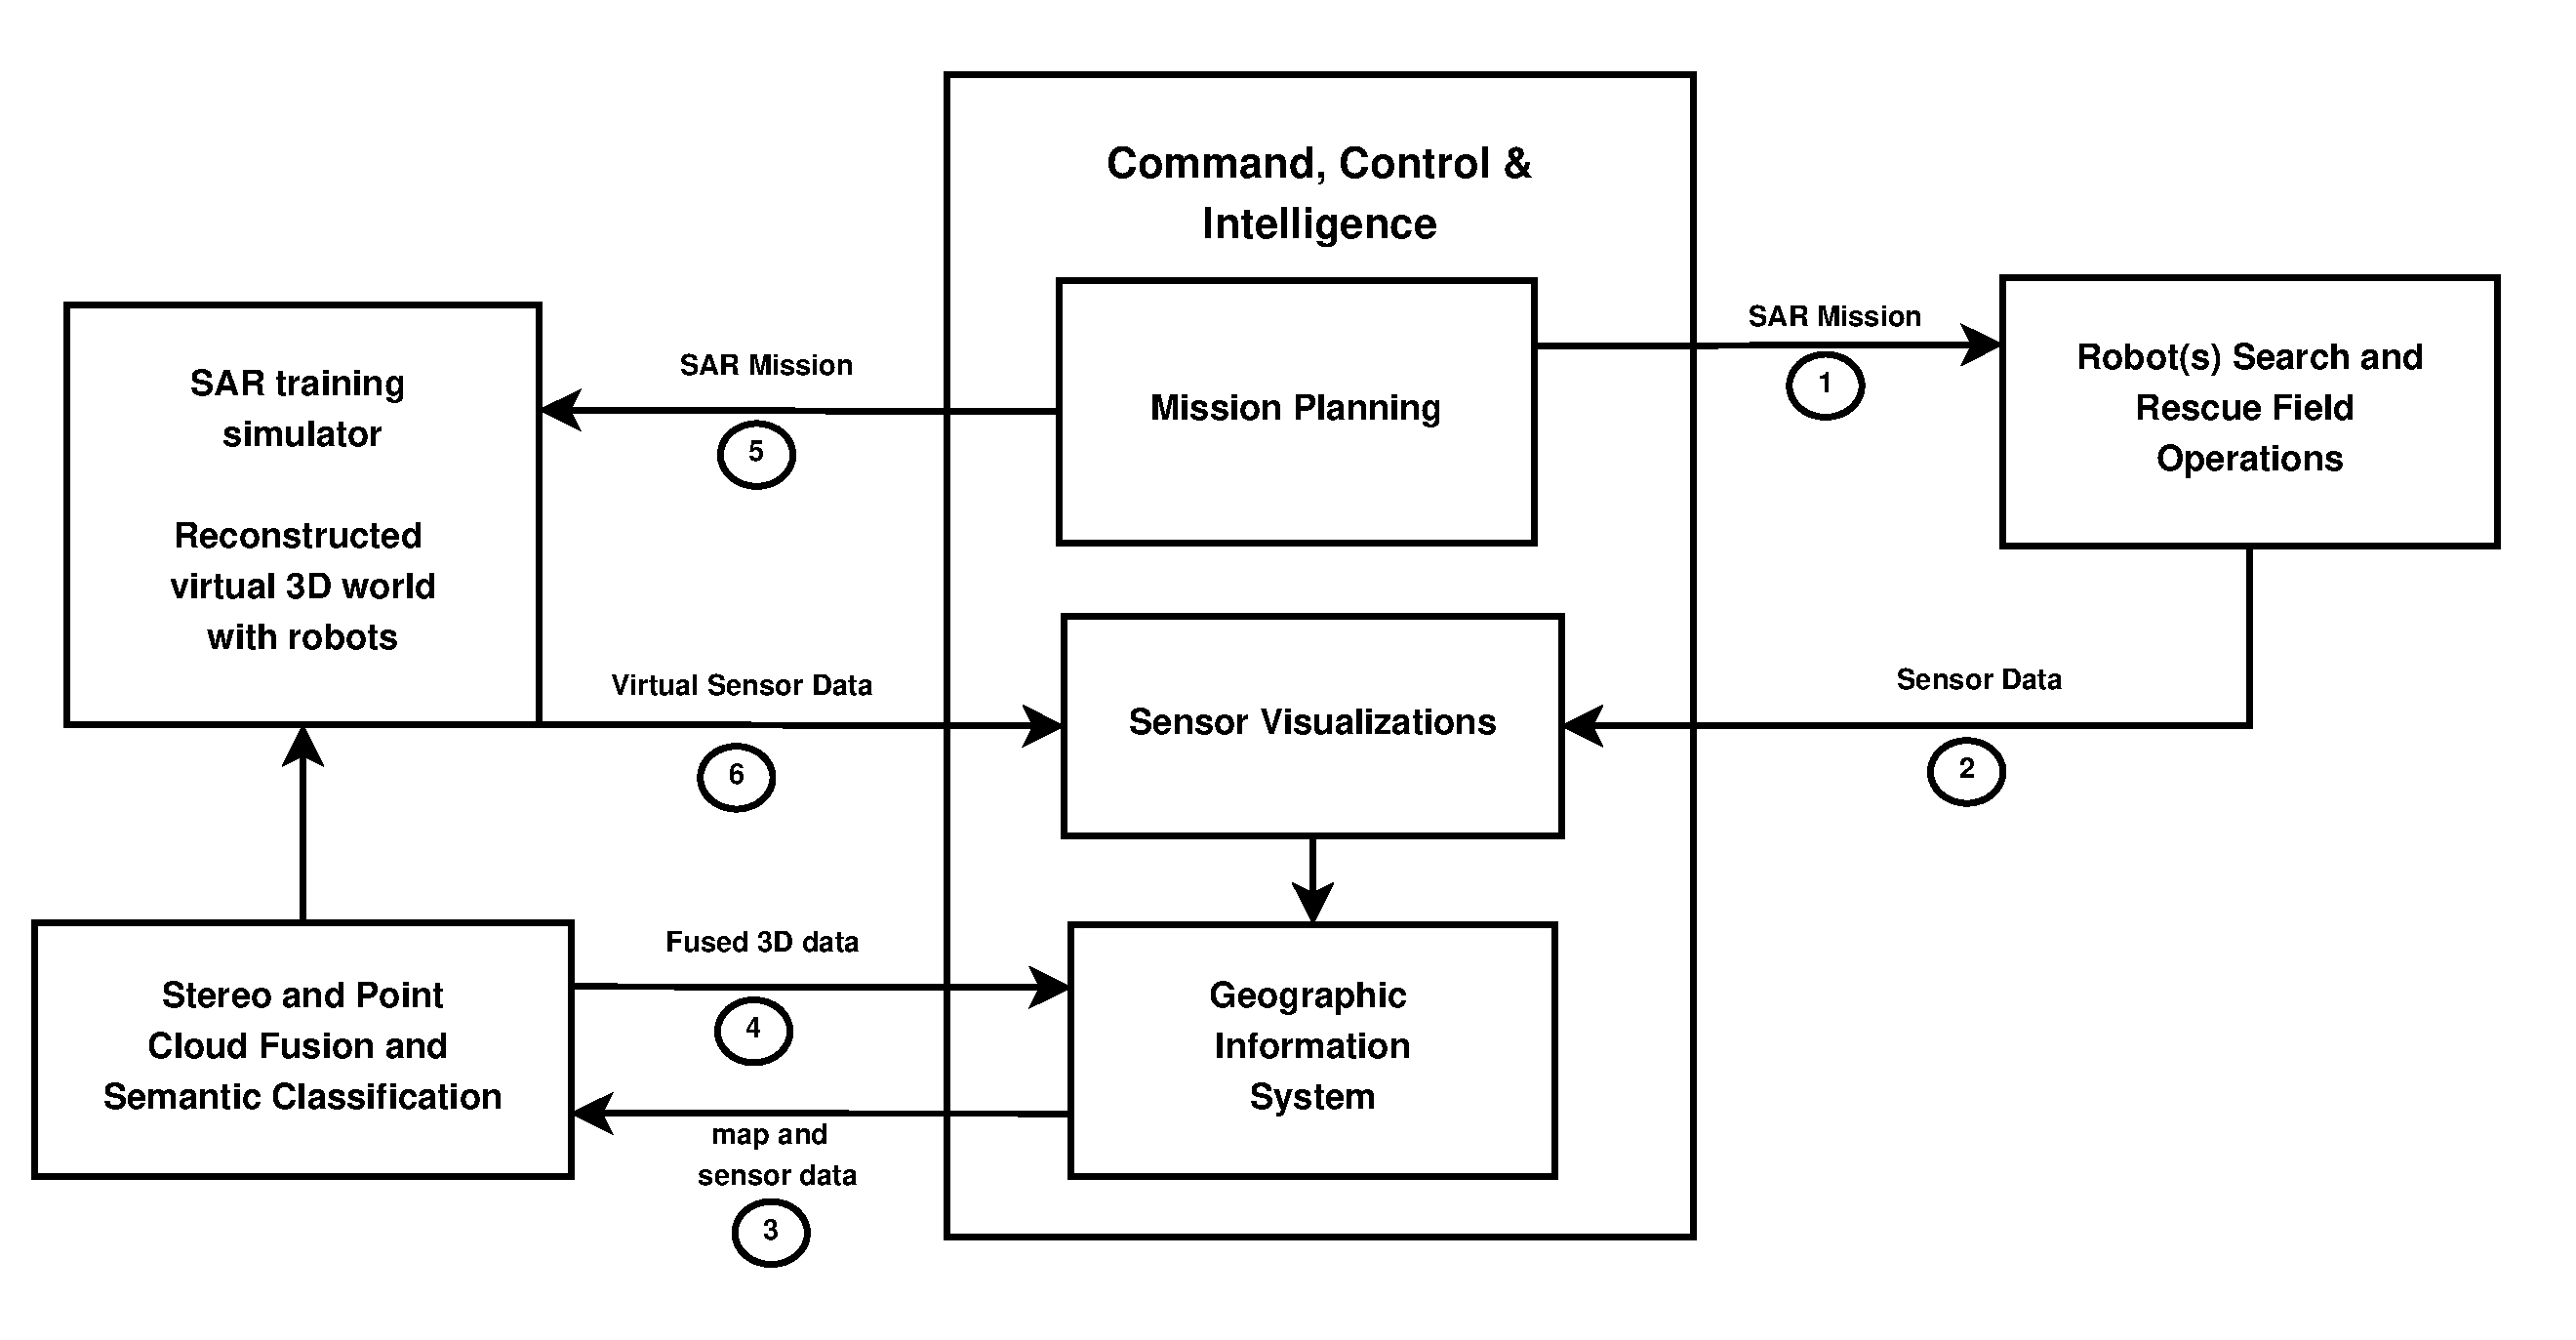
\includegraphics[width=\textwidth]{ROB-15-0035_fig13.eps}
    \caption{Closed loop robot control between real and virtual environments.}
    \label{fig:c2i_real_virtual_flow}
\end{figure}


\afterpage{\clearpage}

\section{Experimental Results}
\subsection{Experimental context}
In the framework of this paper, we present experimental results carried out between 6.09.2014 and 13.09.2014 at the Camp Roi Albert, one of the largest military bases of the Belgian Defence (located near the city of Marche--en--Famenne, Belgium). The same base serves as a SAR training center of the B-FAST (Belgian First Aid and Support Team), which made it ideally suited for experimental SAR tests.
\subsection{Search and Rescue Hardware}
\subsubsection{Unmanned Aerial Vehicles}
The use of UAVs search and rescue missions provides benefits for users due to their low cost, portability, and potential fields of use \cite{tomic}.
In the context of search and rescues missions such systems can offer important support to human task forces in situation assessment and surveillance and in this way increasing the situational awareness of the environment from the air.
The UAVs can be deployed without the need for extensive airstrips for take-off and landing. Operating costs are typically low, compared to conventional manned aircrafts.
The use of small UAVs may improve the response time and coverage for search and rescue operations allowing search and rescue teams to systematically survey and perform mapping of areas (high level of details and accuracy of ground pixel size 2-5 cm) of importance in real time without any physical interaction within dangerous zones \cite{Erdos}\cite{Nagai}.
As every crisis is different and imposes different operational constraints and conditions \cite{URD}, there is no single type of UAV which is able to perform all kinds of missions.
Therefore, multiple types of platforms were considered in the scope of this paper.


The first UAV system corresponds to an extreme endurance solar--powered fixed--wing aerial vehicle. The particular platform is called AtlantikSolar \cite{AtlantikSolarSite} and has been developed by ETH Zurich towards robust multi--day autonomous operation in several scenarios.
AtlantikSolar has a $5.6\textrm{m}$ wingspan, weighs $6.5\textrm{kg}$, is able to fly approximately $12\textrm{h}$ without any solar--charging and perform multi-day flight once appropriate sunlight conditions are available.
As a system it employs  state-of--the--art robust state--estimation capabilities~\cite{LMAS_MSC_14}, automatic trajectory tracking control~\cite{OMLAS_MED_14} while it further integrates an advanced sensor pod built around a monocular version of the tightly syncronized Visual--Inertial sensor system (VI--Sensor)~\cite{nikolic2014synchronized} developed by ETH Zurich and Skybotix AG~\cite{SkybotixSite}.
The AtlantikSolar sensor pod specifically integrates an Aptina MT9V034 camera mounted at a $50^\circ$ front--down oblique view interfaced by the combined Intel Atom--board/FPGA system of the VI--Sensor while each camera frame is annotated with complete pose information.
Additionally, the AtlantikSolar further integrates a GPS--tagged Sony HDR-AS100VW camera. Figure~\ref{AS_P_wSensorPod} depicts the UAV as well as the sensor pod.
As the AtlantikSolar corresponds to a fixed--wing configuration and its sensory systems are mounted in both nadir (facing down) as well as oblique (front--down) configurations, navigation for area perception is preferably handled automatically.
To help the end--user of the platform, automatic viewpoint selection is implemented and the aircraft paths are designed such that a given area is definitely covered at full.
The implemented algorithm accounts for the minimum turn radius of the vehicle, its maximum descending and ascending rates as well as the selected camera configuration.
Essentially, this enables the use of such a highly capable platform via the simple selection of areas to be inspected (provided as Lattitude-Longitute-Altitude GPS coordinates).
Overall, all on--board functionalities relevant to automatic flight are implemented in the employed PX4 Autopilot~\cite{PIXHAWKSite} that runs a modified firmware that implements advanced estimation and control algorithms~\cite{LMAS_MSC_14}\cite{OMLAS_MED_14}.
On the other hand, advanced functionalities take place on--board the aforementioned sensor pod and the INTEL Atom board it integrates.
Communication with other robots and the ground control station is supported via a Telemetry link operating at $433\textrm{MHz}$ that employs the MAVLink protocol~\cite{PIXHAWKSite} as well as a Wi-Fi functioning at $5.2\textrm{GHz}$link.
Manual control is possible at any point via a $2.4\textrm{GHz}$ remote--control link and multiple receivers on--board to maximize robustness and therefore safety.

\begin{figure}
    \centering
    \includegraphics[width=0.7\textwidth]{ROB-15-0035_fig14.eps}
    \caption{The AtlantikSolar UAV with the sensor pod attached to its wings and further photos of the sensor pod, the solar cells and an instant of the hand--launching.}
    \label{AS_P_wSensorPod}
\end{figure}

The second experimental UAV system used in this work is a small vertical take-off aerial system md4-1000 from Microdrones as shown in Figure \ref{fig:UAV}.
This UAV is a quadrotor-based aerial system, with 1030mm diameter and complete carbon body with a maximum payload of around 2kg.
The four gearless brushless electric motors are powered by lithium batteries.
The autopilot is built on a small micro-processor collecting aerodynamics information through a set of tightly coupled sensors (GPS module, 3D-magnetometer, 3-axis gyroscope, 3-axis accelerometer and a barometric pressure sensor), allowing to fly autonomously waypoint-based flights.
The system comprises of a field control base station with high gain antenna for providing command, control and data recording to and from the UAV system.
The field control base station is housed in a ruggedized case in order to protect the equipment.
All data (GPS data, UAV position and attitude data, video data, flight time and battery level data) are transmitted in real-time to the ground receiver station via 5.8GHz wireless communication.
The UAV system is equipped with a Sony NEX-7 24.3 megapixel digital camera with an 18mm lens. The camera is mounted below the UAV on a 2-axis gimbal with high precision tilt and roll stabilization in real time to provide better images for aero triangulation and mapping.
Moreover, it should be noted that the UAV does not fly if the wind speed is higher than 10 m/s.
The digital camera was pre-calibrated in order to obtain good accuracy and results.
\begin{figure}[h]
\centering
\includegraphics[angle=0,width=0.7\textwidth]{ROB-15-0035_fig15}
\caption{Microdrones MD4-1000 quadrotor with field control base station.}
\label{fig:UAV}
\end{figure}


The third UAV system is an autonomous outdoor coaxial quadcopter.
The platform is called LIFT IV and has been developed by Eurecat Technology Center to satisfy the needs of Search and Rescue operations.
LIFT IV has a 855 mm diameter and weights 4.3 Kg.
The propulsion chain has been optimized to maximize the payload capacity (3.8 Kg), endurance (over 30 minutes) and wind resistance (up to 35 Km/h), allowing to fit to different scenarios and configurations.
The autopilot has been modified and integrated with an onboard computer to enable autonomous navigation capabilities such as obstacle avoidance and autonomous infrastructure inspections.
These features allow the execution of mapping and observation mission in confined scenarios, where regular Ready To Fly platforms are usually forced to operate in manual mode since a priori flight planning is not feasible.
The UAV platform is shown in Figure \ref{fig:UAV2}.
The payload kit integrates several sensors.
A compact Canon IXUS 130 digital camera with 14.1 M provides conventional RGB images.
This camera is mounted in two different configurations: downwards looking for aerial mapping, and oblique (45 degrees) for better buildings 3D reconstruction.
The images from this camera are stored on the camera and only post-processed after landing.
The platform also integrates a Vision-Inertial sensor~\cite{nikolic2014synchronized}, developed by ETH Zurich and Skybotix AG, to enable vision based navigation and grayscale mapping.
Finally, a thermal imager, FLIR Tau2, is also used for mapping, real-time victim detection and to support night operations.
All these later images are captured from the onboard computer and geotagged with the current position and attitude estimation.
This allows future developments towards close to real-time mapping during flight.
\begin{figure}[h]
\centering
\includegraphics[angle=0,width=0.7\textwidth]{ROB-15-0035_fig16}
\caption{Coaxial quadcopter system developed for search and rescue applications.}
\label{fig:UAV2}
\end{figure}

Using these UAVs, geo-referenced orthomosaics and Digital Terrain Models (DTM) can be obtained without the need of having accurately measured ground coordinate values.
However, more accurate geo-referencing does require ground control points.
In dangerous zones, it is impossible to set ground control points, unlike normal aerial surveys.
The addition of the direct geo-referencing method (which does not require ground control points) from a UAV therefore makes this UAV-based mapping system ideally suited for disaster areas and the search and rescues domain.
\subsubsection{UGV Robot System}
The rough outside world and 3D unstructured environment in the domain of SAR applications pose several constraints on the mechanical structure of deployed UGV robot systems, the electronics, the control architecture and on the robustness of the autonomous components.
Next to the technical constraints, an important factor to be taken into consideration is also the economic opportunity of developing a mechanical design for a robotic platform which is focused on one sole task or type of environment, as there may not be a wide enough market for the valorization of this platform. Hence, often platforms with a wider envelope of capabilities and with more flexible capacities are selected, even though these platforms are not always the best in one single task.
For the same reasons as for the UAVs, multiple UGVs were deployed in order to gather data from the outdoor environment and from within indoor structures.


The first UGV system consists of a heavily modified Telerob tEODor Explosive Ordenance Disposal (EOD) robot ~\cite{EODTeodor}.
This search and rescue UGV robot system shown in Figure ~\ref{fig:tEODorbasic} was developed in the context of the EU-FP7-ICARUS project ~\cite{ICARUS} to serve as an experimental evaluation platform and was upgraded with the necessary  electronics,  sensors, computing power, motor control units and power sources in order to be able to execute remote-controlled and semi-autonomous tasks.
In order to provide required perceptual data input for environmental perception and navigation assistance, a depth sensing system was integrated on the UGV, as show in Figure ~\ref{fig:tEODorbasic}.
This exteroceptive 3D sensing system consists of a VisLab 3DV stereoscopic camera ~\cite{itsc2013} system and a 360 rotating SICK LMS-100 laser rangefinder, which was coupled to a GPS-INS system (the IG-500N from SBG systems), providing accurate geo-localization to all acquired data.
This platform has proven its usefulness in dealing with rough and different types of terrains (mud, gravel, grass, rocks, sand) with excellent maneuverability and good off-road performance through its tracked system.
The platform has a useful payload capacity of around 100 kg, making it capable of carrying an extensive and flexible sensory payload and on-board processing equipment, depending on the application.
The rugged and rain resistant design of the platform makes it capable of handling unfriendly environmental conditions.
Currently, the robot tracks are powered by two electro motors, allowing the UGV robot system a top speed of 3km/h and to climb stairs and ramps up to 45 degrees.
The platform is able to operate up to 3 hours in mixed operation conditions.
More information about this platform can be found in \cite{HarisPP} \cite{Haris2}.
\begin{figure}[h]
\centering
 \begin{subfigure} [lt]{0.54\textwidth}
 \centering 
         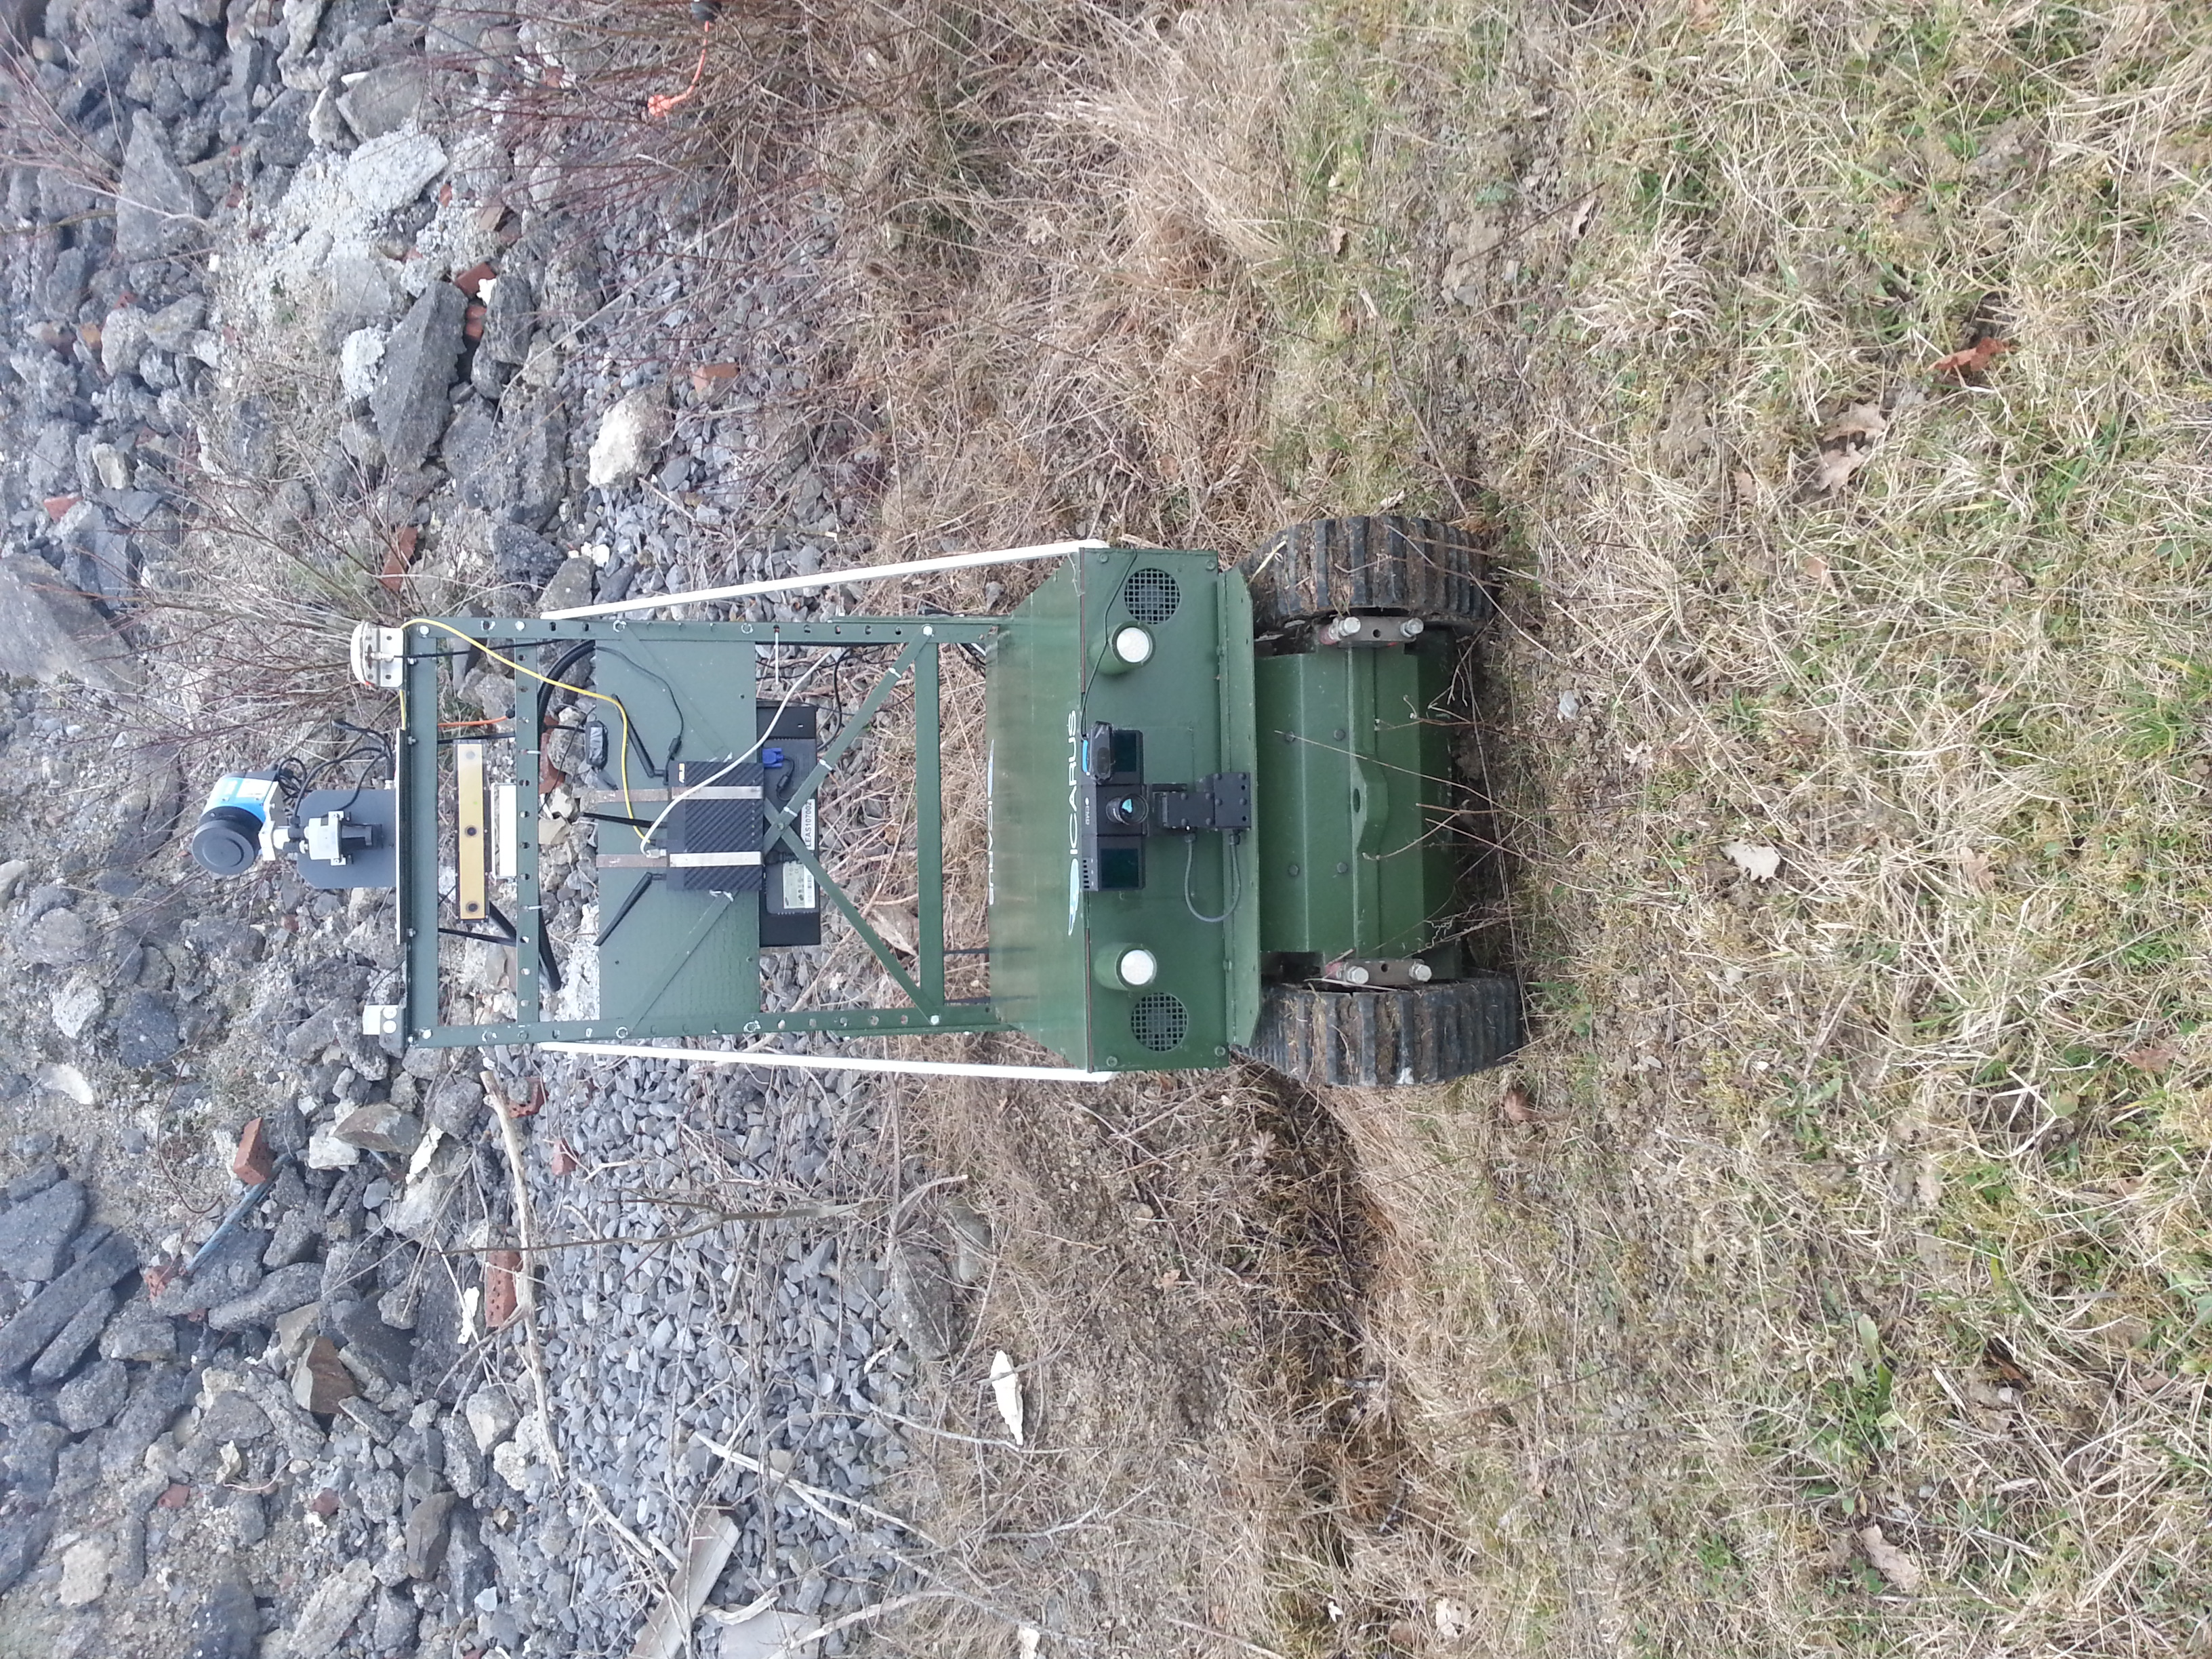
\includegraphics[scale=0.09,angle=270,origin=c]{ROB-15-0035_fig17a}
 \end{subfigure}
  \begin{subfigure} [rt]{0.44\textwidth}
  \centering 
         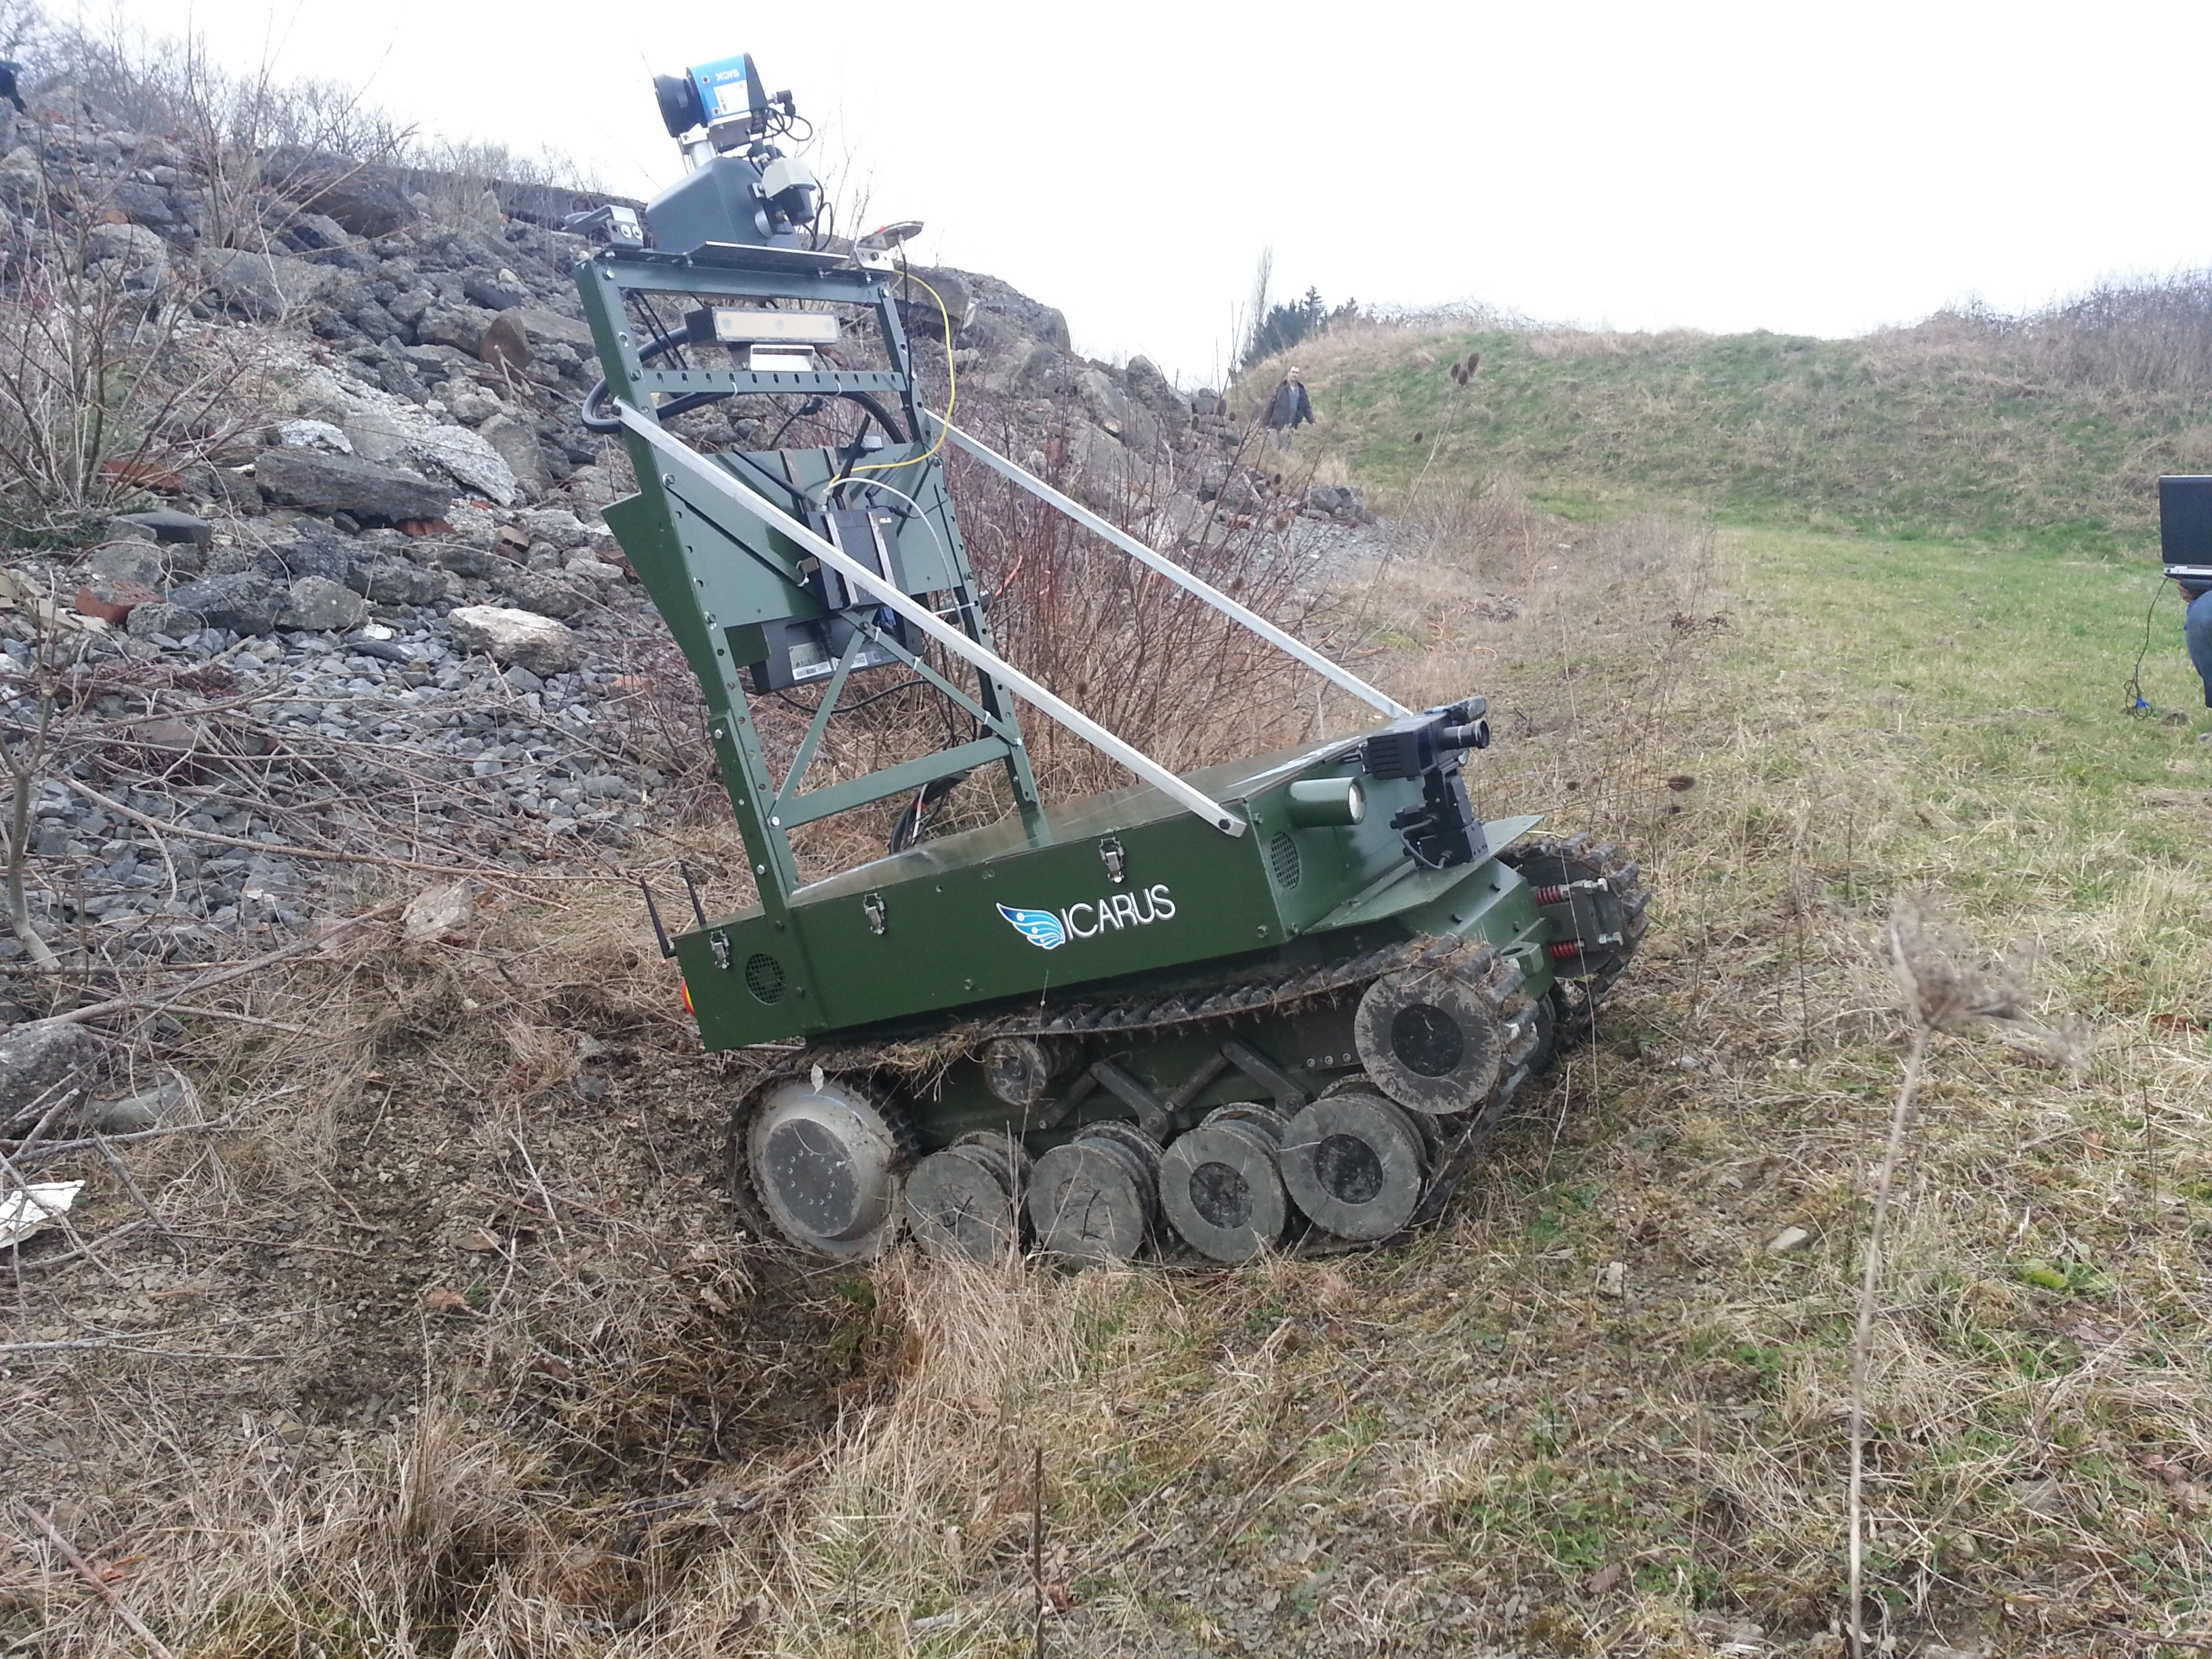
\includegraphics[scale=0.06]{ROB-15-0035_fig17b}
         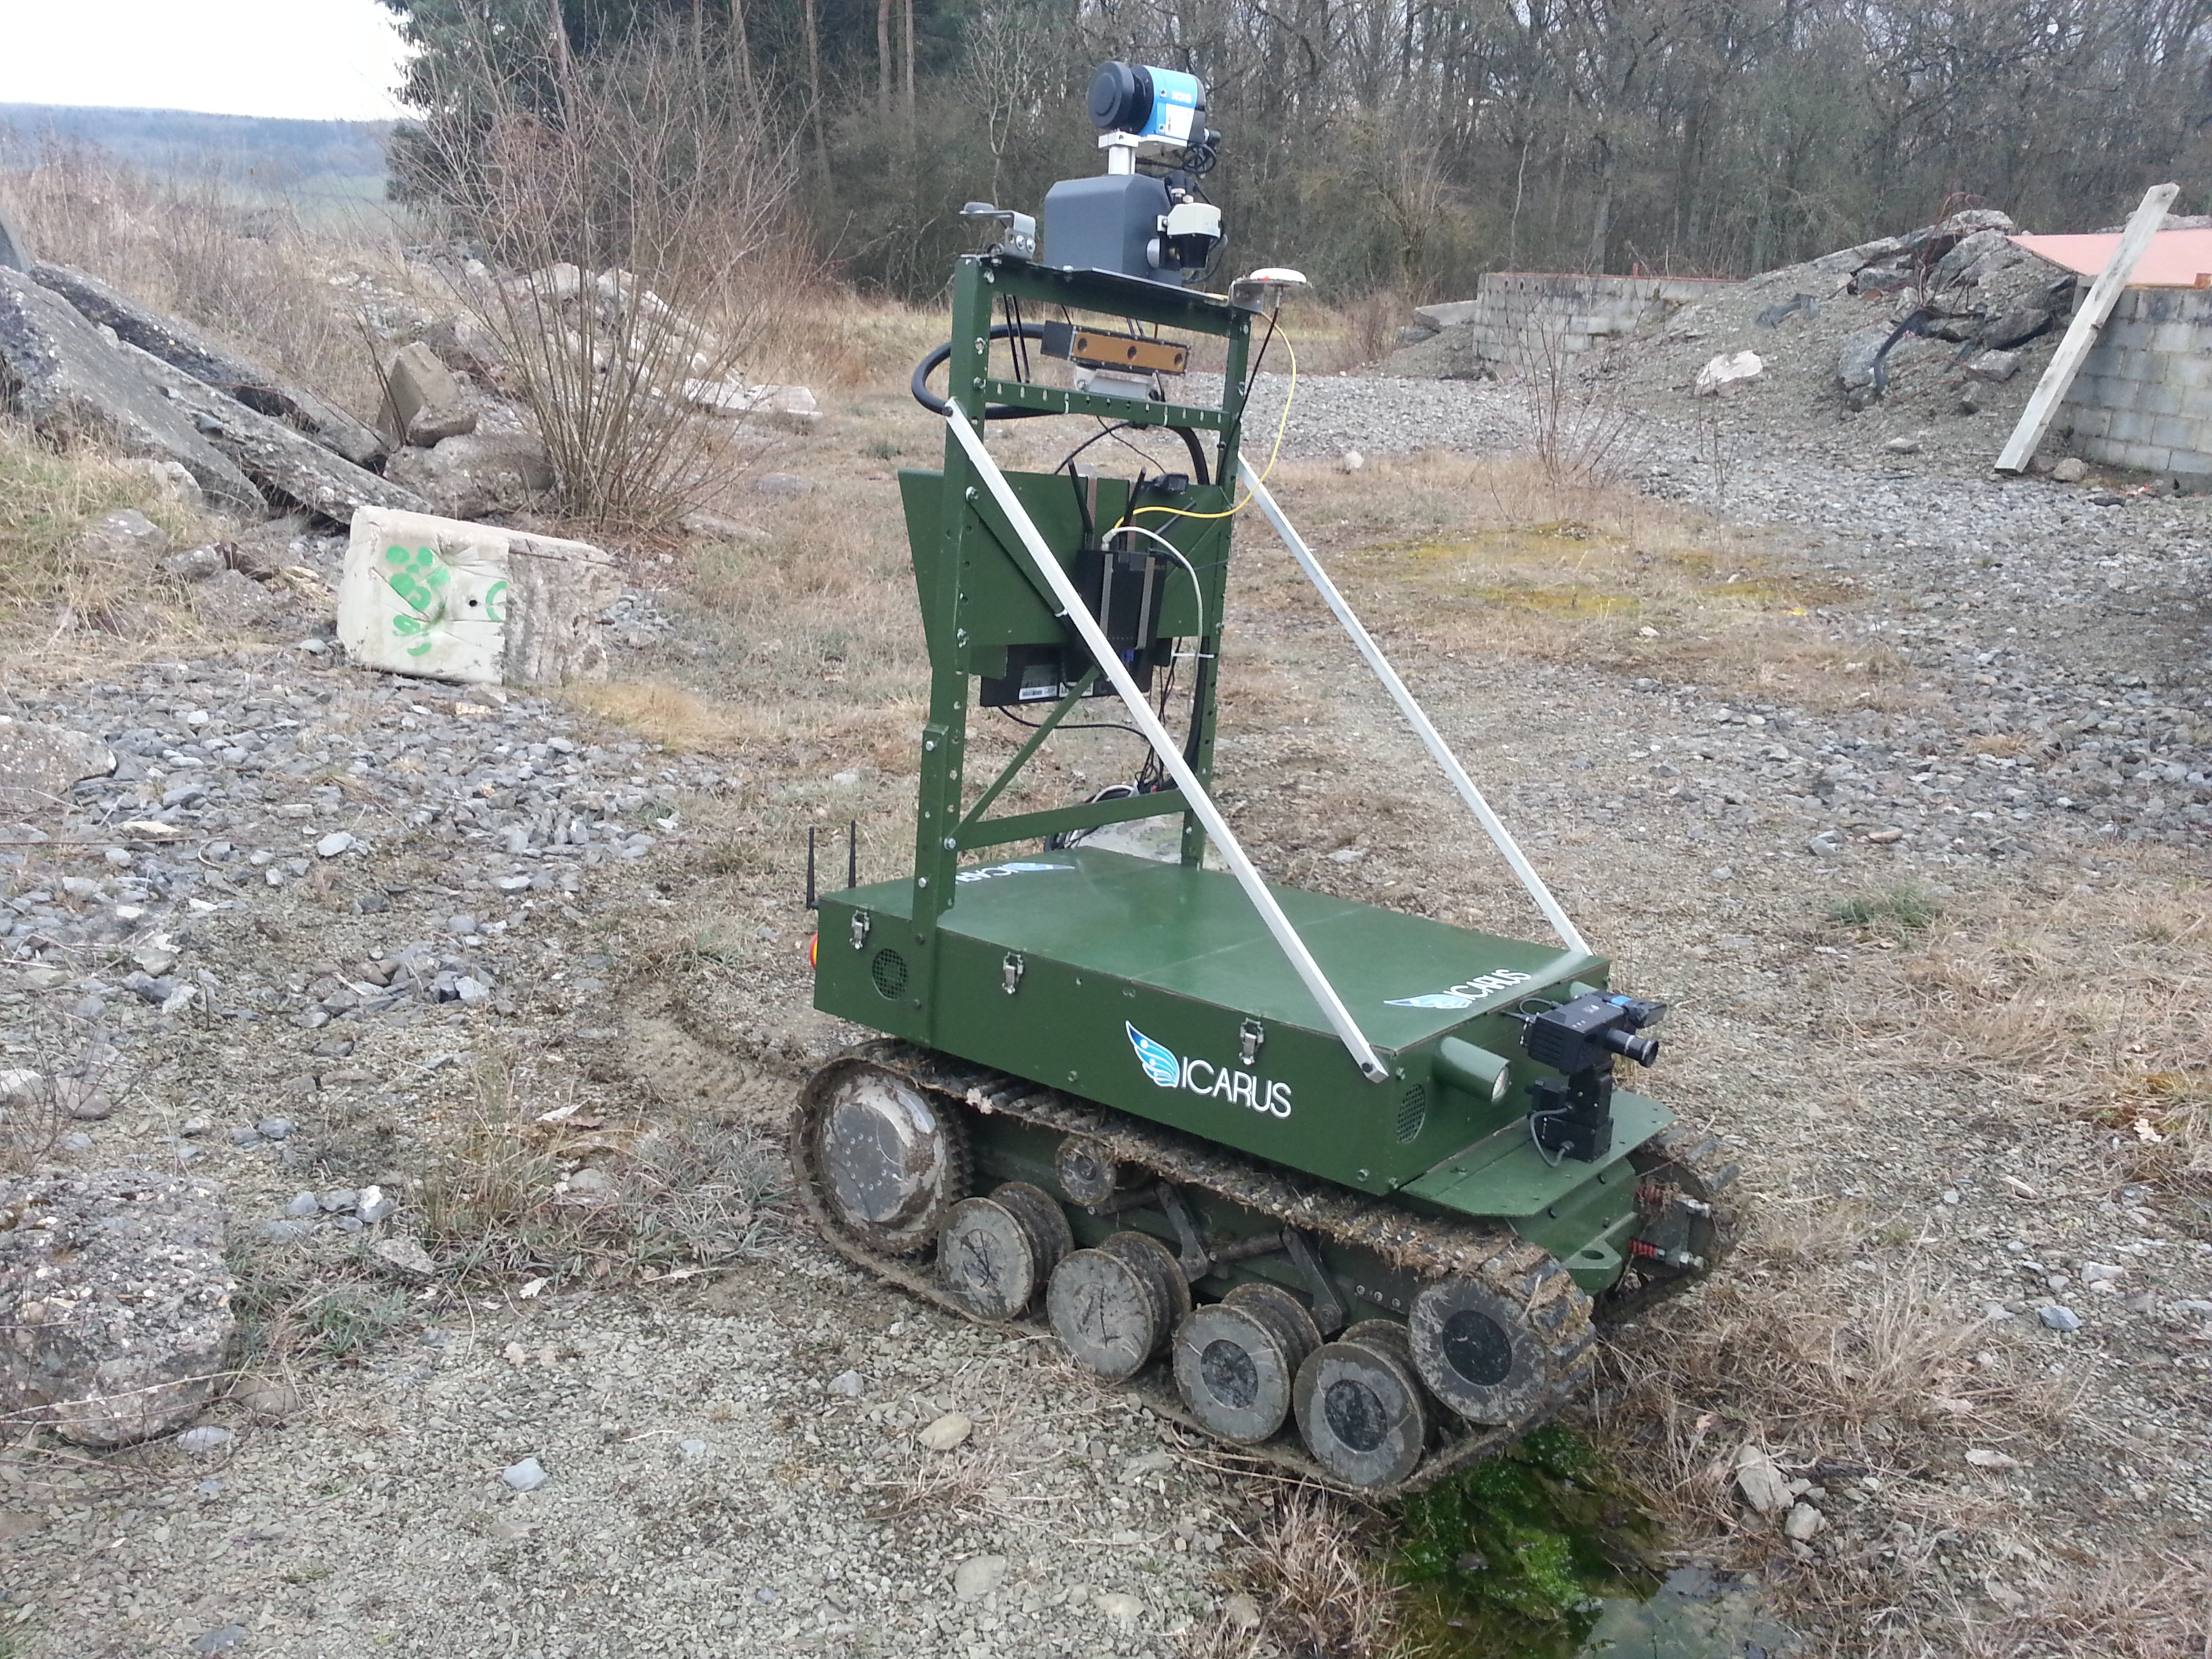
\includegraphics[scale=0.06]{ROB-15-0035_fig17c}
 \end{subfigure}

\caption{Picture of the SAR UGV used for experimental evaluation (FP7-285417 ICARUS project) and a view of the sensor setup (a VisLab 3DV stereoscopic camera system ~\cite{itsc2013} and a 360 rotating SICK LMS-100 laser rangefinder).}
\label{fig:tEODorbasic}
\end{figure}

For the experiments shown in this paper we have also used two other platforms:
\begin{itemize}
\item A Dr-Robot Jaguar 4x4 equipped with laser 3D scanner based on rotary SICK LMS 100, as shown on figure \ref{fig:drrobot}.
\item A Husky platform equipped with geodetic laser system Z+F IMAGER 5010, as shown on figure \ref{fig:husky}. Data from Z+F IMAGER was used for creating virtual environment for training tools.
\end{itemize}
The main goal of these platforms is to help in exploring the area and gather data necessary for building the 3D maps.
The Dr-Robot platform is dedicated for fast scanning of buildings from the outside and the inside.
The Husky platform is a part of the training and support system and carries high accuracy laser scanner for gathering precise data.
Gathered maps can later be used for creating realistic training environments.
As for now both platforms are tele-operated.
\begin{figure} [h]
    \centering
    \begin{subfigure} [br]{0.4\textwidth}
         \centering
         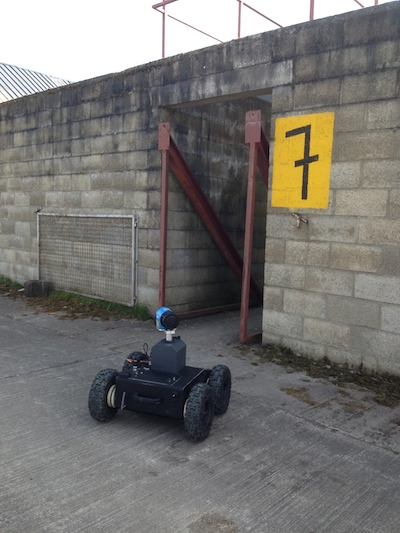
\includegraphics[scale=0.55]{ROB-15-0035_fig18a.png}
         \caption{Dr-robot Jaguar 4x4}
         \label{fig:drrobot}
    \end{subfigure}
    \begin{subfigure} [bl]{0.4\textwidth}
         \centering
         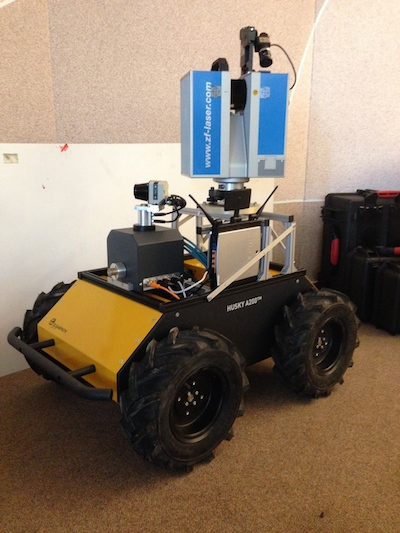
\includegraphics[scale=0.55]{ROB-15-0035_fig18b.png}
         \caption{Husky}
         \label{fig:husky}
    \end{subfigure}%
    \caption{ICARUS UGV SAR Hardware.}
    \label{fig:SARrobotichardware}
\end{figure}
\subsection{Command and Control Station} \label{command_and_control}
The robot command and control station is responsible for planning missions for exploration and mapping a disaster site by unmanned systems.
The control station hardware in Figure \ref{fig:RC2_BOX} consists of a wheel portable ruggedized Pelican Hardigg case which houses a consolidated set of systems such as a rugged laptop, communications management Mini-ITX computer, dual band WiFi antennas (2.45 and 5.2 Ghz) mounted on a telescopic stand, Garmin GPS receiver, secondary outdoor viewable screen, two rugged hall effect joysticks, a wireless gamepad controller, modular battery slabs with onboard power control units, splash proof ventilation ducts with fans, external power socket and lighting for operations during the night.
The rugged laptop hosts the robot command and control software and is interfaced with the secondary display and communications hardware.
The GPS receiver provides the global position of the control station to be indicated in the user interface and to the communications systems for network management between deployed nodes.
The control station can be transported easily in harsh surface conditions due to the rubber mounted shock absorbing frame housing all the components in the lower lid and the precision cut high density foam housing components for quick access to users in the upped lid of the case.
The control station currently provides around 6 hours of autonomy without external power sources and the endurance can be increased with the addition of battery slabs, which affects its portability due to an increases the weight of the case.
The case with all its components weighs approximately 25kg and has dimensions of length: 94.4cm,  breadth: 53cm and height: 31.6 cm, which is within the deployment requirements as indicated by the Belgian First Aid and Support Team (B-FAST).
\begin{figure}
    \centering
    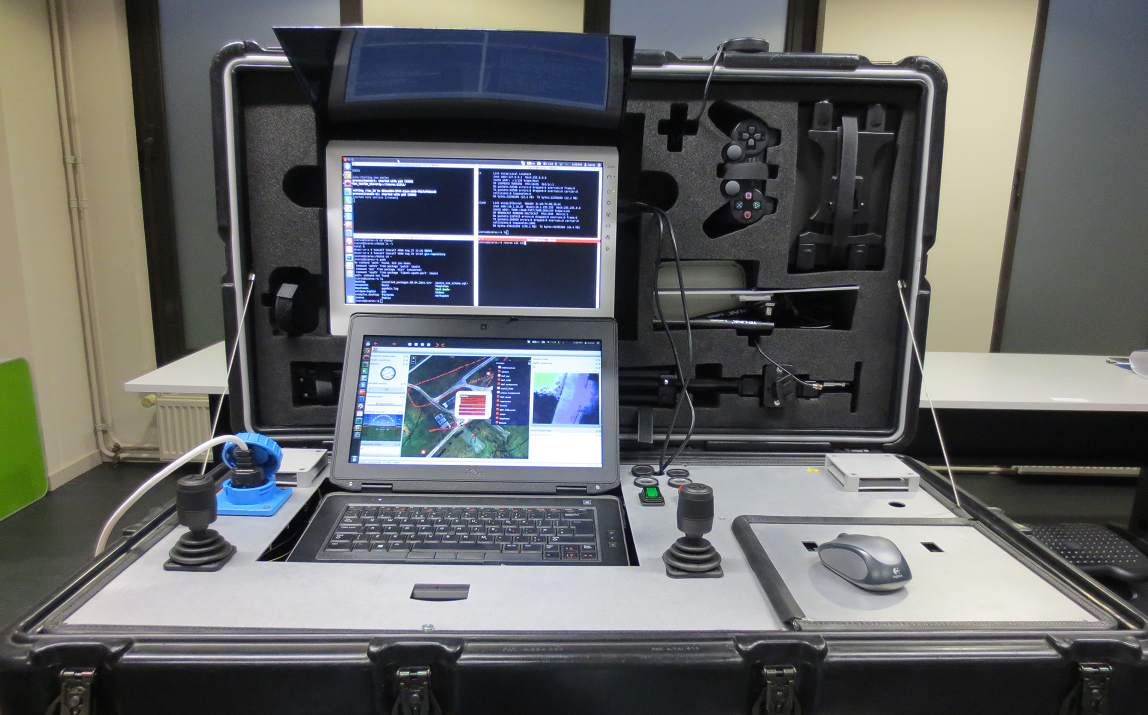
\includegraphics[width=\textwidth]{ROB-15-0035_fig19.png}
    \caption{Robot command and control portable base station.}
    \label{fig:RC2_BOX}
\end{figure}


\subsection{Mission Planning and Robot Command and Control}\label{mission_planning}

The portable robot control station equipment was first deployed on the field.
The UAVs and UGVs were paired with the C2I and deployed for mapping the assumed--to--be disaster area at Marche--en--Famenne, Belgium.
On launching the C2I, the robots operating within the range of the network are automatically detected and their location and global orientation are indicated on the map.
Views for displaying the robot specific network link qualities, battery level, orientation, cameras, raw point clouds and the overall generated point clouds are simultaneously initialized as shown in Figure~\ref{fig:c2i_ugv_trials}.
A set of waypoints are charted on the map as a reference path by the robot operator who was located as a fixed position. Regarding the use of the AtlantikSolar fixed--wing system, the waypoint list generation is automatically achieved via a path--planner that guarantees full coverage of the desired area while respecting the aircraft minimum turn radius, maximum ascending and descending rates as well as the on--board camera(s) configuration.
On the other hand, the ground robot’s trajectory was controlled using a standard gamepad while referring to sensor visualizations.
Local trajectory planning by the operator was influenced by limitations imposed on the UGV by the terrain such as the roll and pitch, energy consumption and network quality.
Data from odometry, cameras and Lidar were recorded in the GIS and as rosbags for post-processing. Figure~\ref{fig:c2i_ugv_trials} demonstrates the C2I in operation with a UGV and Figure~\ref{fig:c2i_IMMSim_cam} shows a few views of the C2I during field operation with UAV's.
\begin{figure}
    \centering
    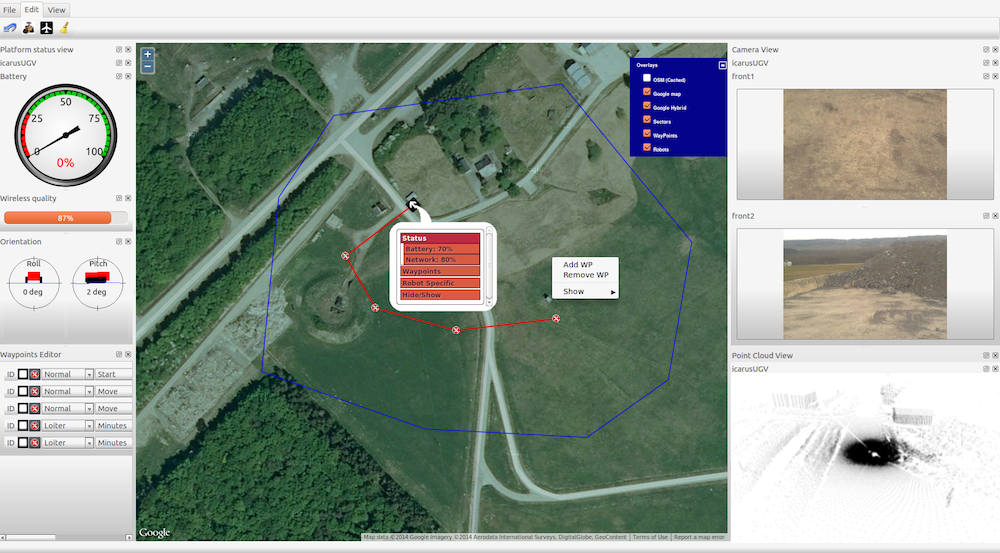
\includegraphics[width=\textwidth]{ROB-15-0035_fig20.png}
    \caption{UGV trials.}
    \label{fig:c2i_ugv_trials}
\end{figure}
\subsection{Data gathered by individual platforms}
In order to explain to the reader which is the content of the dataset we are releasing with this paper, this section describes the data which was individually gathered by the different platforms in the scope of a search and rescue simulation exercise.
\subsubsection{AtlantikSolar UAV}
An example inspection path and a sparse version of the corresponding point cloud derived using the Pix4D software~\cite{Pix4Dsite} is shown in Figure~\ref{fig:AtlantikSolar_Inspection}.
This data was gathered while the vehicle remained airborne for more than $5\textrm{h}$ continuously during the public trial event.


\begin{figure}
    \centering
    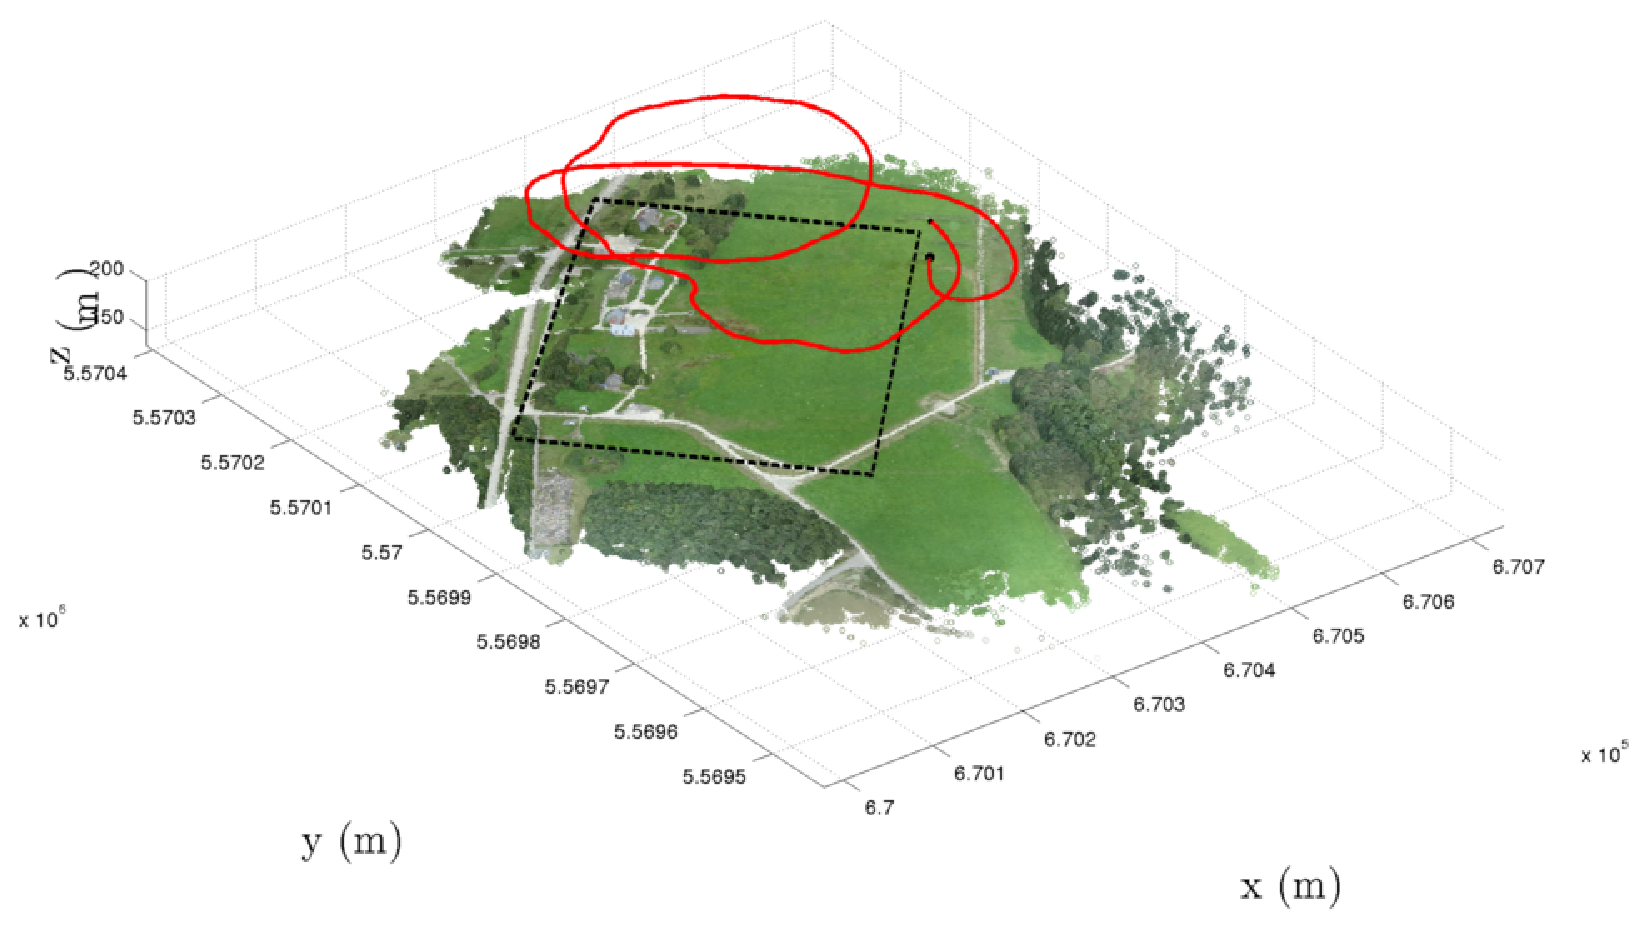
\includegraphics[width=\textwidth]{ROB-15-0035_fig21.eps}
    \caption{Inspection mission conducted by AtlantikSolar in the area of Marche--en--Famenne.
The inspection mission reference waypoints and the recorded flight path are plotted along the computed dense point clouds of the desired area to be explored using the RGB Sony Camera on--board the UAV.
The derived maps come with geoinformation and were computed with the assistance of the Pix4D software. The point cloud is here presented in a sparse form and using ENU coordinates.}
    \label{fig:AtlantikSolar_Inspection}
\end{figure}


\subsubsection{MicroDrones MD4-1000 UAV}
Aerial photographs were acquired by autonomous waypoint-based flight.
The software we use to produce the preprogramed flight plan and to post-process the data is the ORBIT UAS Mapping software.
The flying height of UAV was around 75 m above ground and with 33 minutes of flight time we covered more than $250.000m^2$ of interest area as shown in Figure \ref{fig:ppFpo}. The flight was executed with 6 straight line strips, because of the low altitude flying height we could achieve a ground pixel size around 1.5 cm with a photo-overlap of 60-80 \% and acquired 566 photos in total shown in Figure \ref{fig:claio}. Figure \ref{fig:pic} shows example images acquired by the UAV system.

\begin{figure}[h]
 \begin{subfigure} [b]{0.49\textwidth}
         \centering
         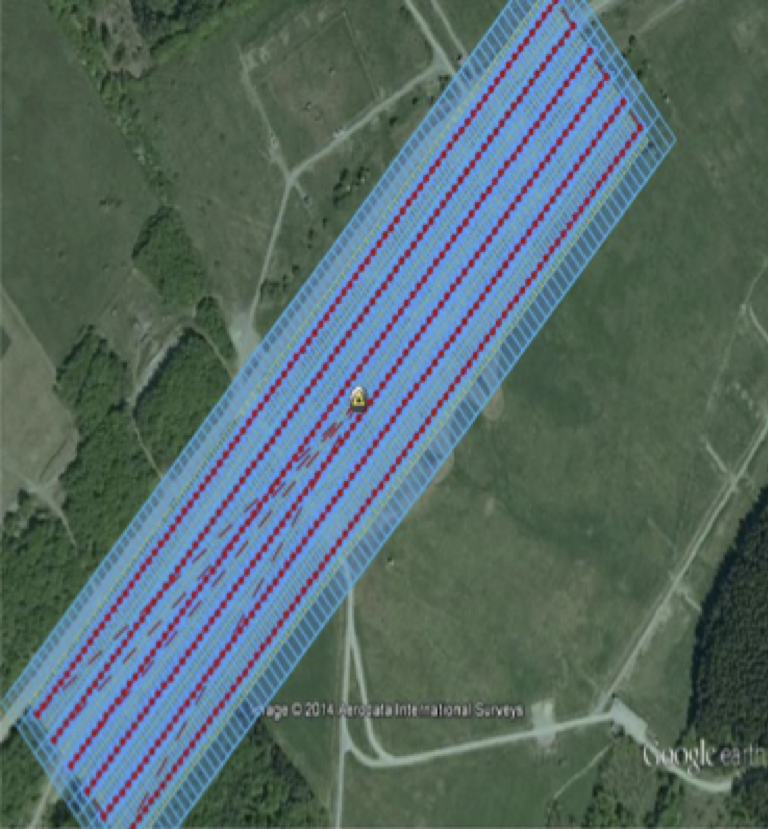
\includegraphics[scale=0.6]{ROB-15-0035_fig22a.png}
         \caption{Pre-programed flight plan over Marche-en-Famenne Military Base.}
         \label{fig:ppFpo}
 \end{subfigure}
 \begin{subfigure} [b]{0.49\textwidth}
         \centering
         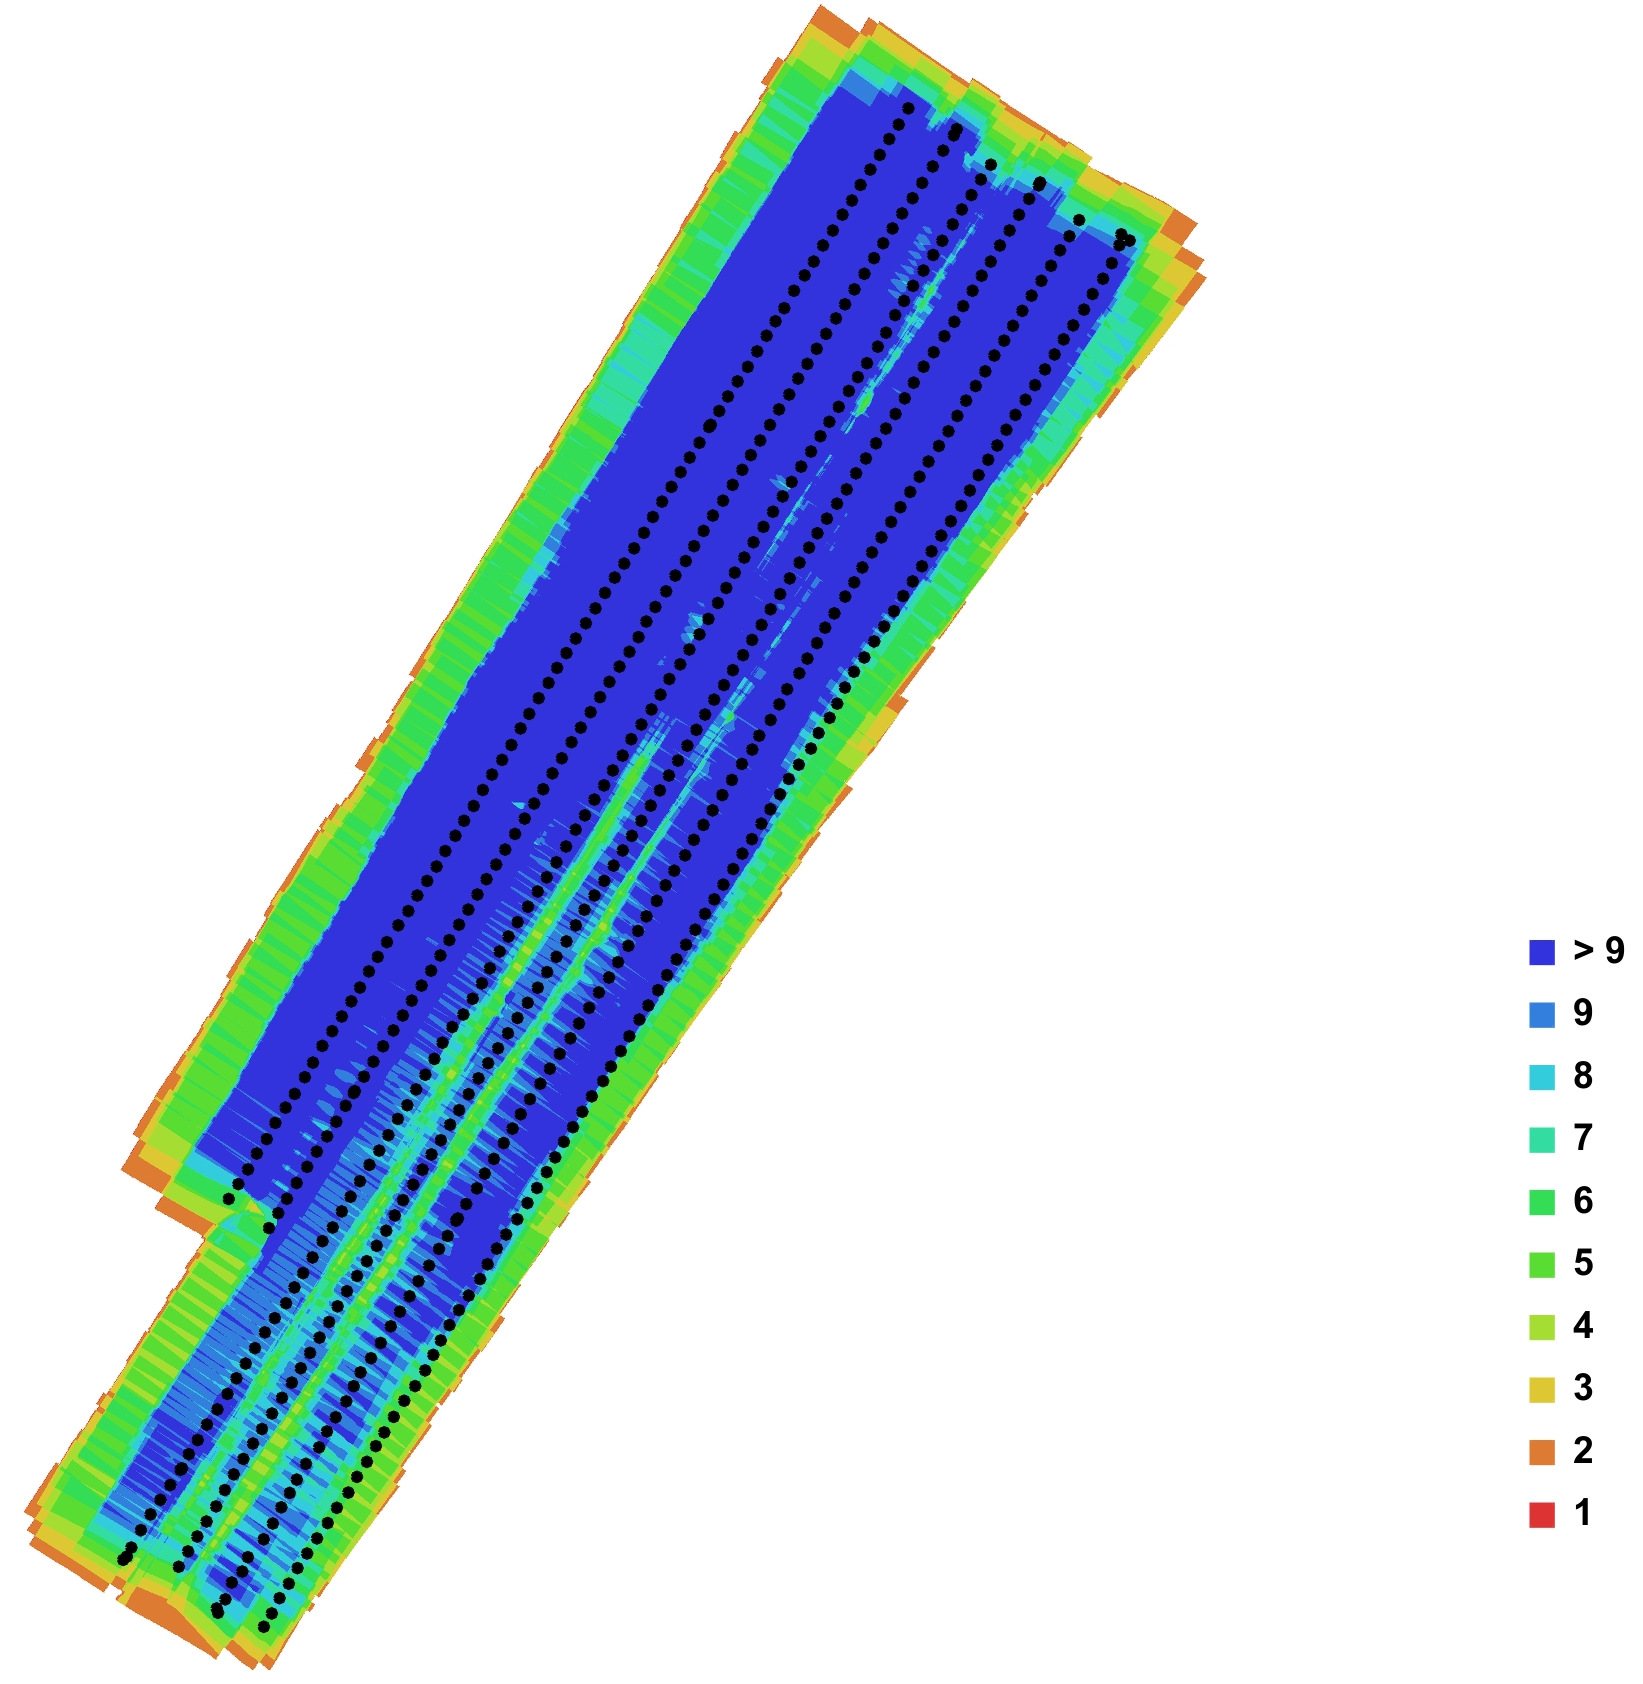
\includegraphics[scale=0.14]{ROB-15-0035_fig22b.jpg}
         \caption{Camera locations and image overlap.}
         \label{fig:claio}
 \end{subfigure}
 \caption{Area of Interest.}
\label{fig:hrun}
\end{figure}

\begin{figure}[h]
\centering
 \begin{subfigure} [b]{0.24\textwidth}
         \includegraphics[scale=0.018]{ROB-15-0035_fig23a}
 \end{subfigure}
  \begin{subfigure} [b]{0.24\textwidth}
         \includegraphics[scale=0.018]{ROB-15-0035_fig23b}
 \end{subfigure}
  \begin{subfigure} [b]{0.24\textwidth}
         \includegraphics[scale=0.018]{ROB-15-0035_fig23c}
 \end{subfigure}
  \begin{subfigure} [b]{0.24\textwidth}
         \includegraphics[scale=0.018]{ROB-15-0035_fig23d}
 \end{subfigure}
  \begin{subfigure} [b]{0.24\textwidth}
         \includegraphics[scale=0.018]{ROB-15-0035_fig23e}
 \end{subfigure}
  \begin{subfigure} [b]{0.24\textwidth}
         \includegraphics[scale=0.018]{ROB-15-0035_fig23f}
 \end{subfigure}
  \begin{subfigure} [b]{0.24\textwidth}
         \includegraphics[scale=0.018]{ROB-15-0035_fig23g}
 \end{subfigure}
  \begin{subfigure} [b]{0.24\textwidth}
         \includegraphics[scale=0.018]{ROB-15-0035_fig23h}
 \end{subfigure}
\caption{Example images acquired by the UAV system.}
\label{fig:pic}
\end{figure}
We generated the ortho-mosaic and DTM using an algorithm, which analyses all images of the aerial data set and searches for matching points.
The most well-known feature matching algorithm is the scale-invariant feature transform approach.
Those feature-matching points are combined with meta-data information from the autopilot (altitude, camera position and orientation) and are used in a bundle block adjustment in order to reconstruct the exact position and orientation of the camera for every acquired image. Based on this reconstruction the matching points are verified and their 3D coordinates calculated.
The coordinate reference system we used was the Belgian Lambert 72 projection. Those 3D points are interpolated to form a triangulated irregular network in order to obtain a Digital Elevation Model (DEM). This DEM is used to project every image pixel and to calculate the geo-referenced ortho-mosaic of the area.
The reconstructed DEM and the resulting ortho-mosaic are shown in Figure \ref{fig:hmap}. The quality of digital ortho-mosaic and DEM depends on the accuracy of the Ground Control Points (GCPs). If the quality of GCPs is excellent, therefore the result of digital ortho-mosaic and DEM can be anticipated accurately too.

\begin{figure} [h]
    \centering
    \begin{subfigure} [b]{0.33\textwidth}
         \centering
         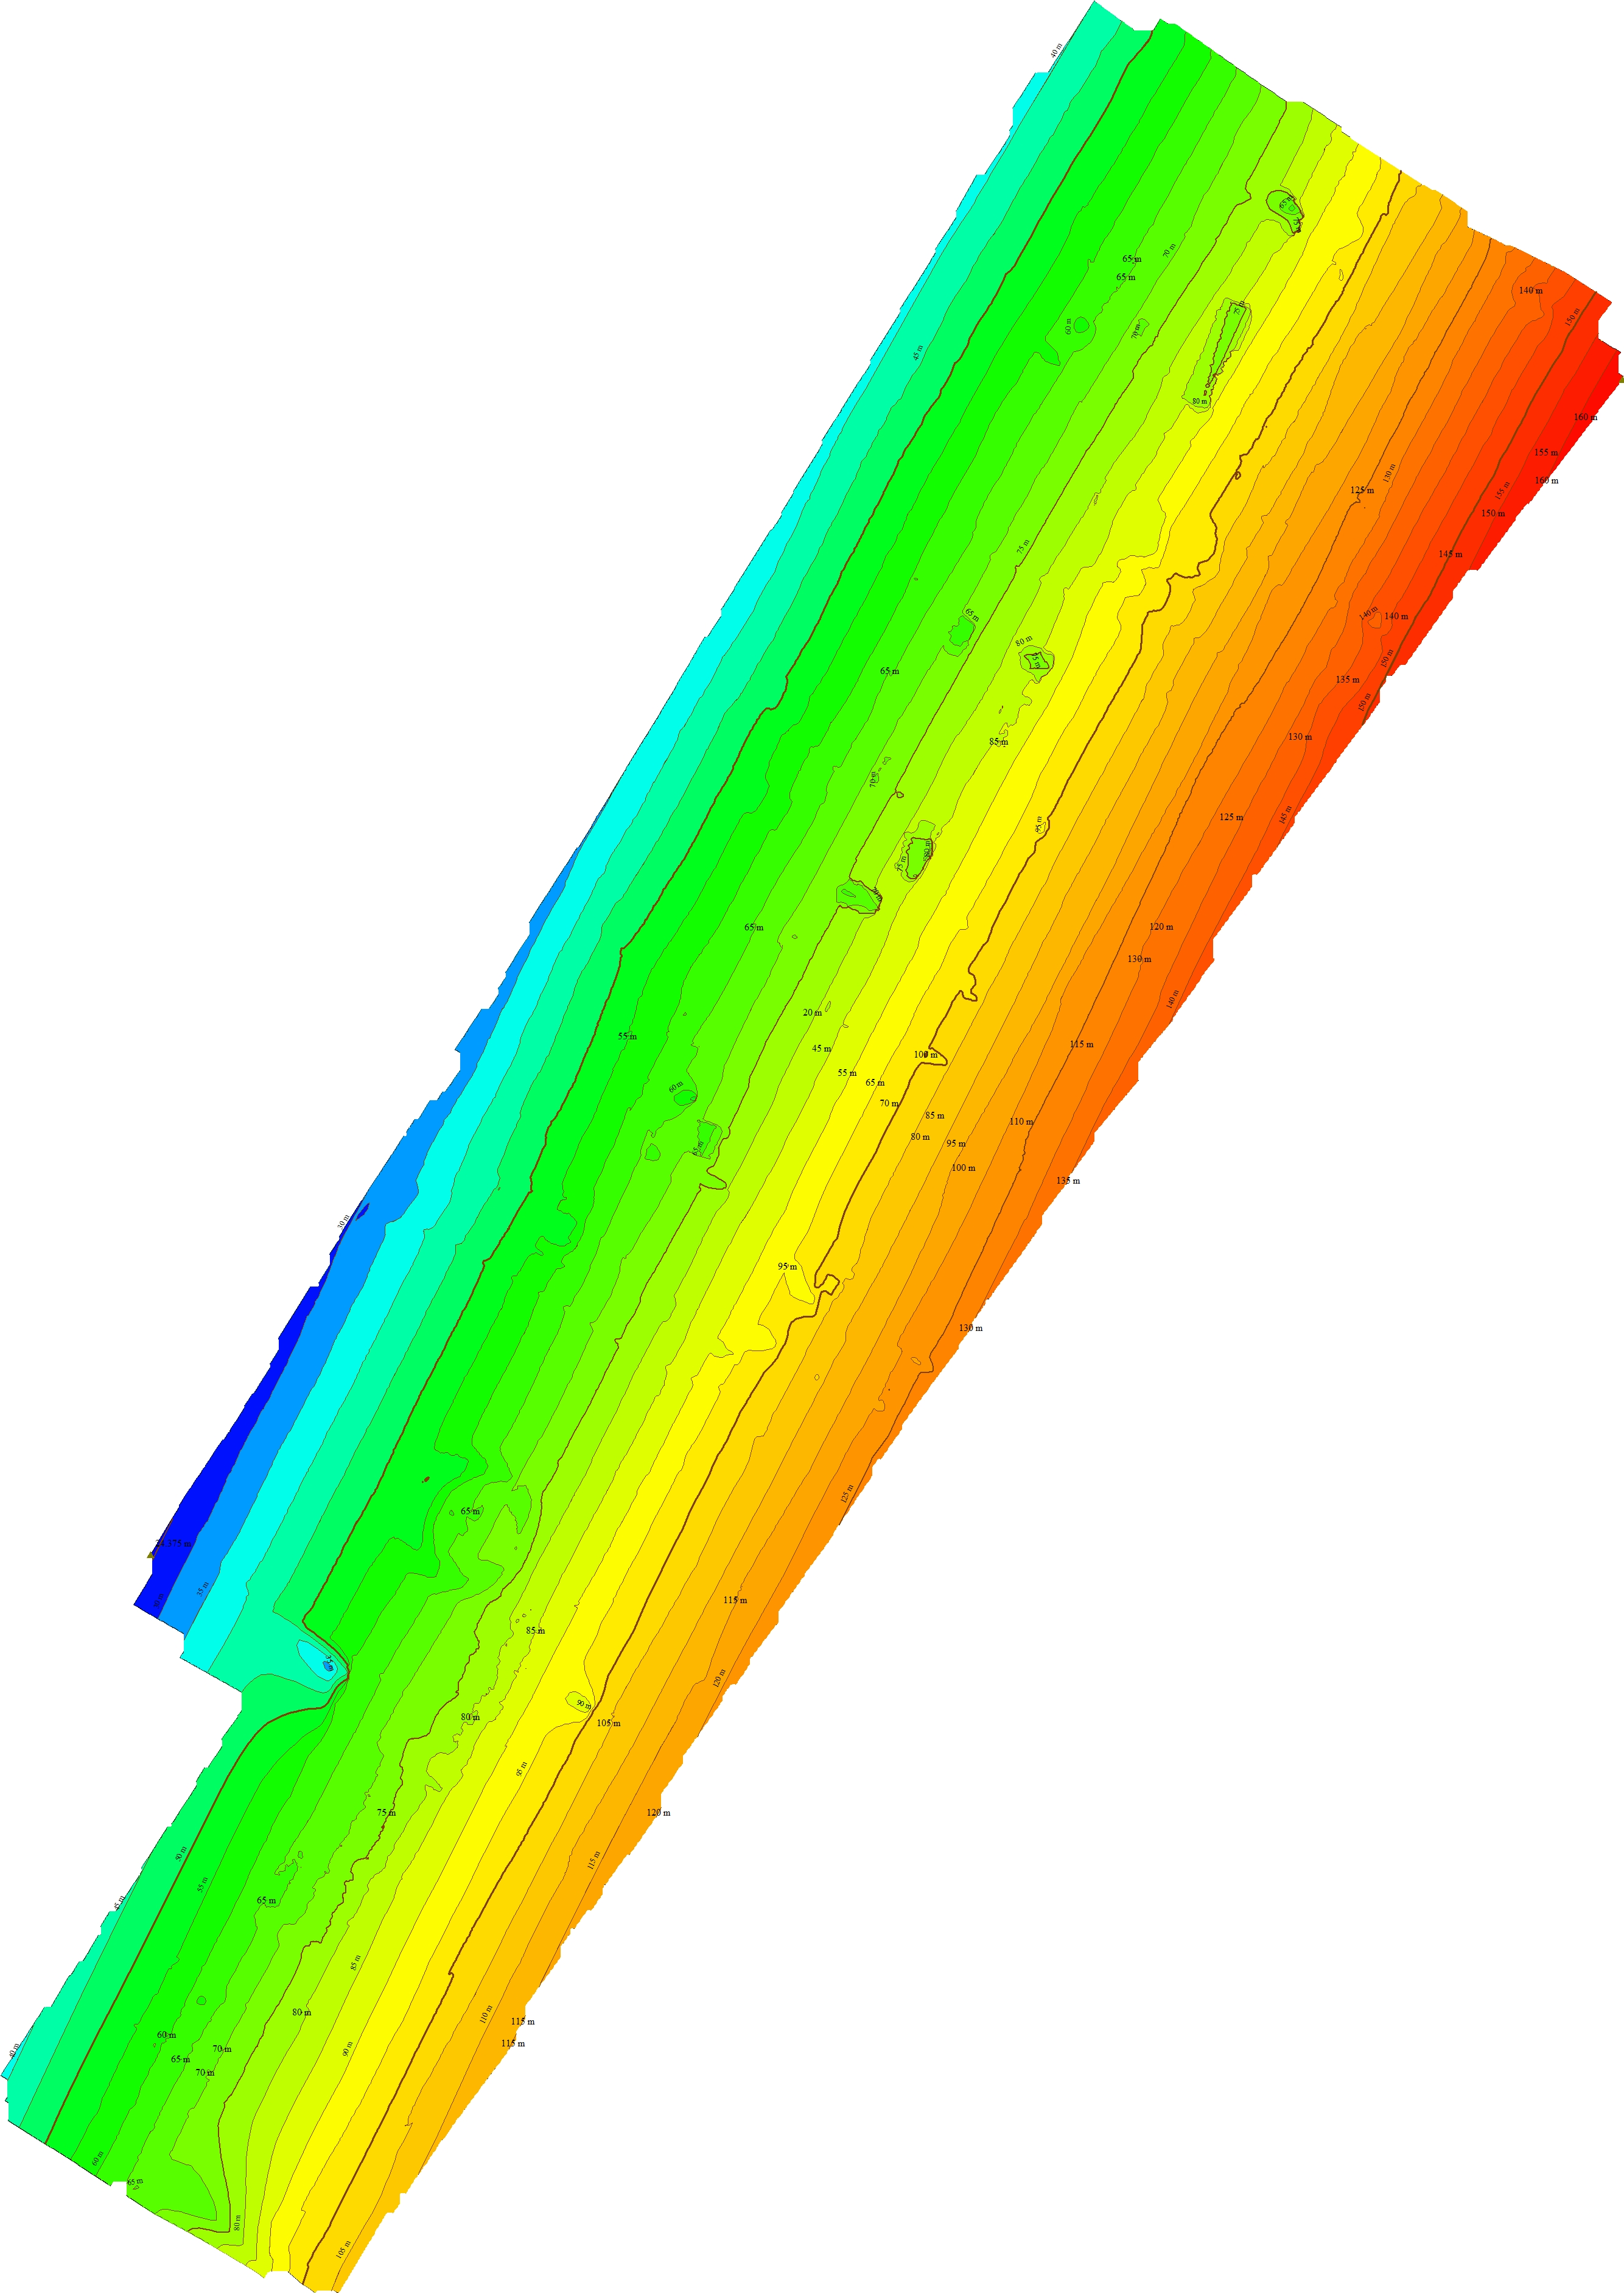
\includegraphics[scale=0.054]{ROB-15-0035_fig24a}
         \caption{Contour DEM}
         \label{fig:aaa}
    \end{subfigure}%
    \begin{subfigure} [b]{0.33\textwidth}
         \centering
         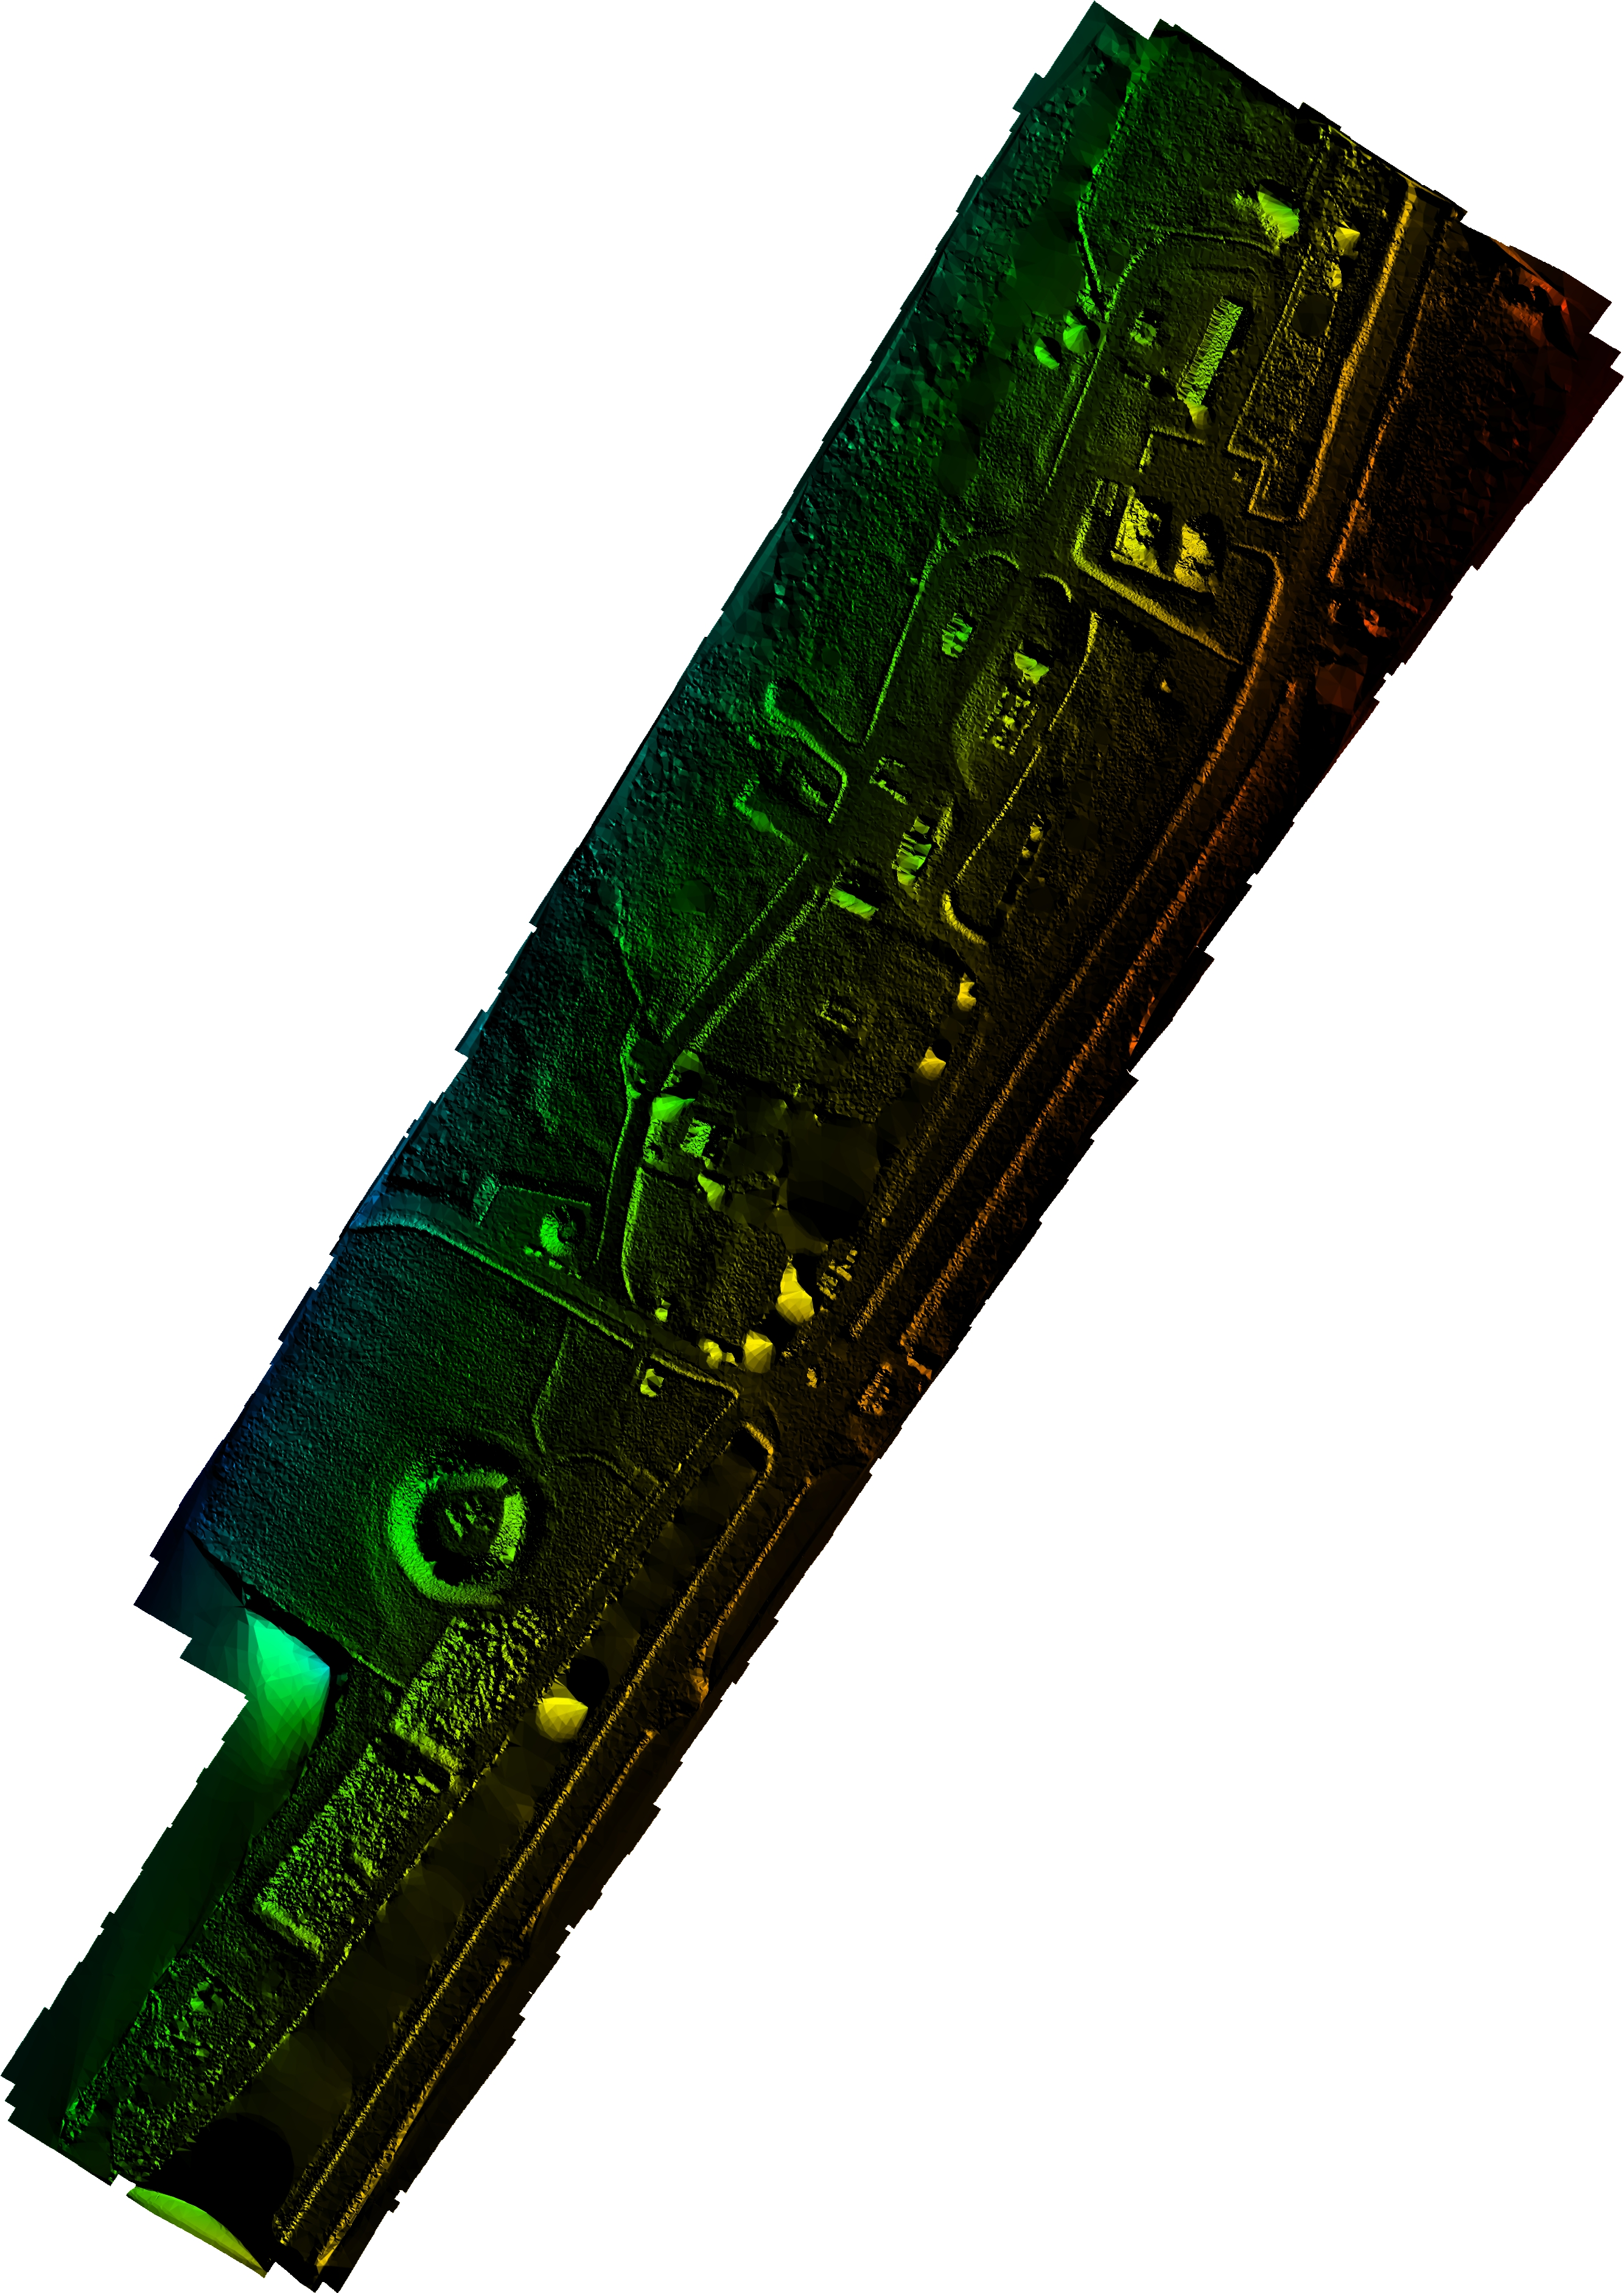
\includegraphics[scale=0.055]{ROB-15-0035_fig24b.jpg}
         \caption{DEM}
         \label{fig:bbb}
    \end{subfigure}
    \begin{subfigure} [b]{0.33\textwidth}
         \centering
         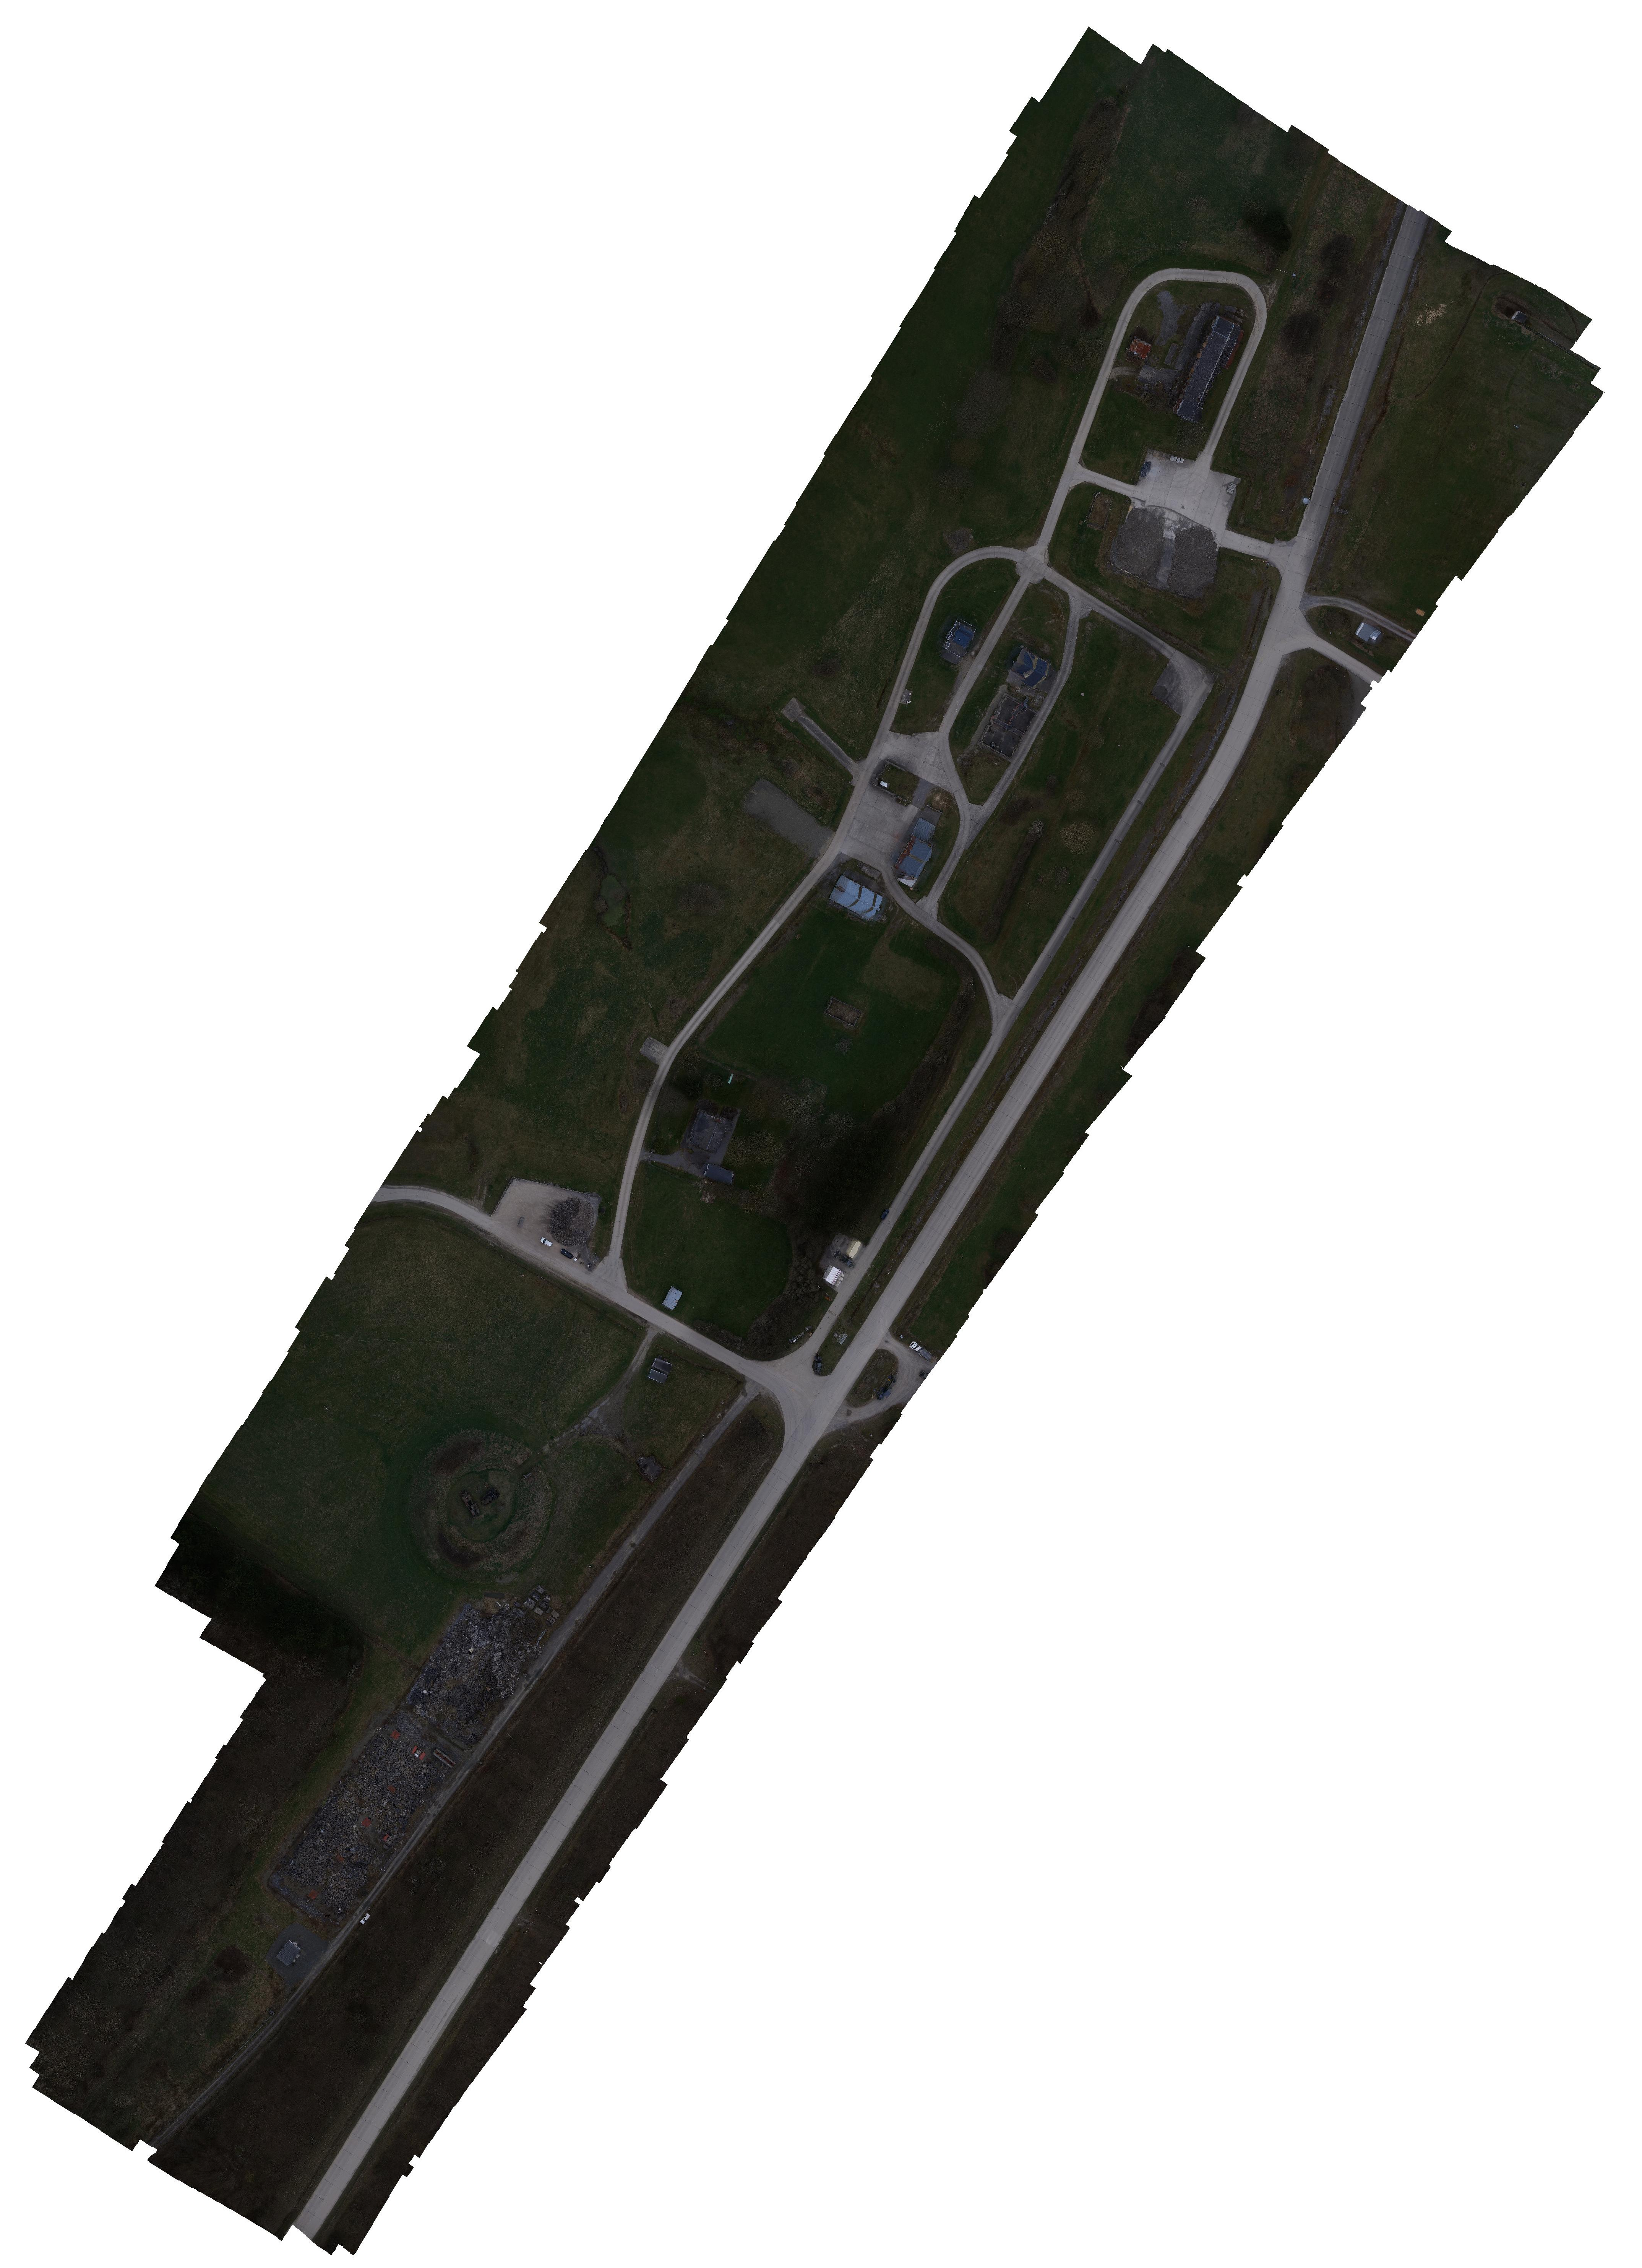
\includegraphics[scale=0.035]{ROB-15-0035_fig24c}
         \caption{Ortho-mosaic}
         \label{fig:cccc}
    \end{subfigure}%
    \caption{Reconstructed digital elevation model and the resulting orthomosaic.}
    \label{fig:hmap}
\end{figure}



\subsubsection{LIFT IV UAV}
Different camera payloads were carried by this platform, ranging from a Canon IXUS 130 camera, over a Aptina MT9V034 camera to a FLIR Tau 2 thermal camera. In all cases, point clouds were generated from the raw data using the Agisoft PhotoScan software, leading to the 3D maps shown on Figure \ref{fig:adata}.
\begin{figure} [h]
    \centering
    \begin{subfigure} [b]{0.49\textwidth}
         \centering
         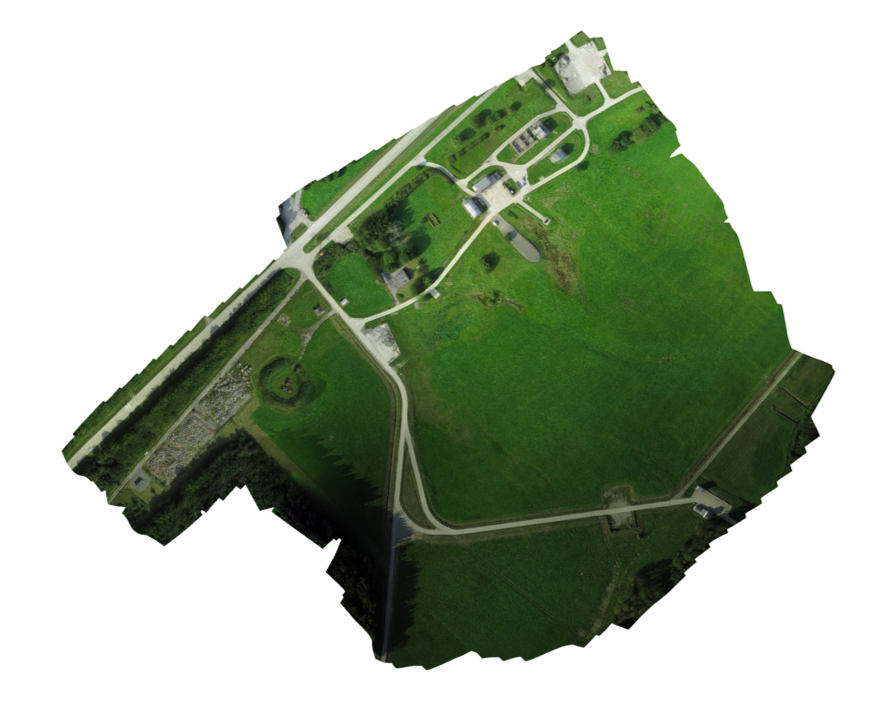
\includegraphics[width=0.9\textwidth]{ROB-15-0035_fig25a.png}
         \caption{Canon IXUS 130 camera}
         \label{fig:ad1}
    \end{subfigure}%
    \begin{subfigure} [b]{0.49\textwidth}
         \centering
         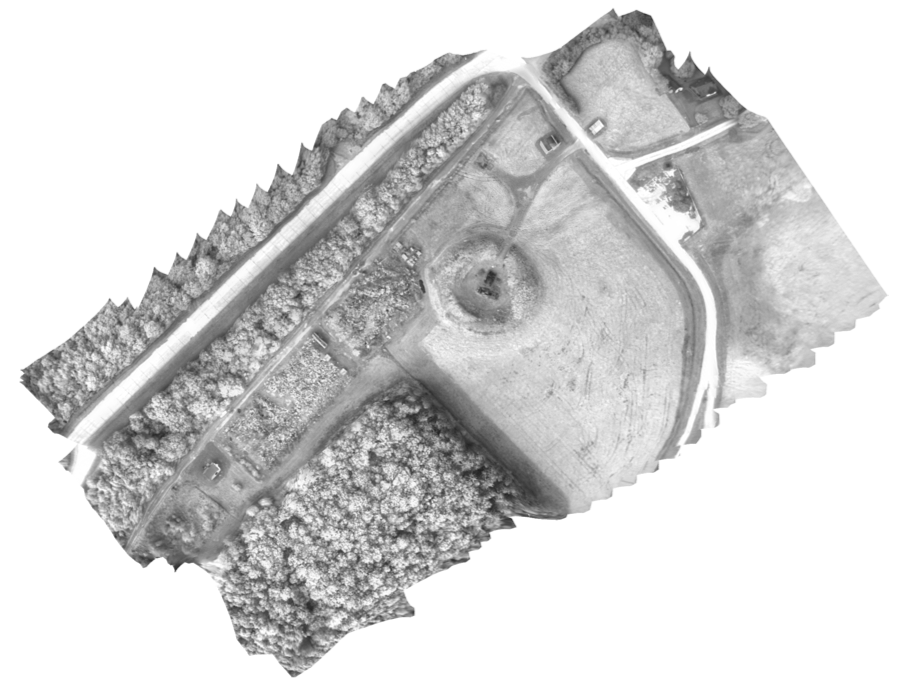
\includegraphics[width=0.9\textwidth]{ROB-15-0035_fig25b.png}
         \caption{Aptina MT9V034 camera}
         \label{fig:ad2}
    \end{subfigure},
    \begin{subfigure} [b]{0.49\textwidth}
         \centering
         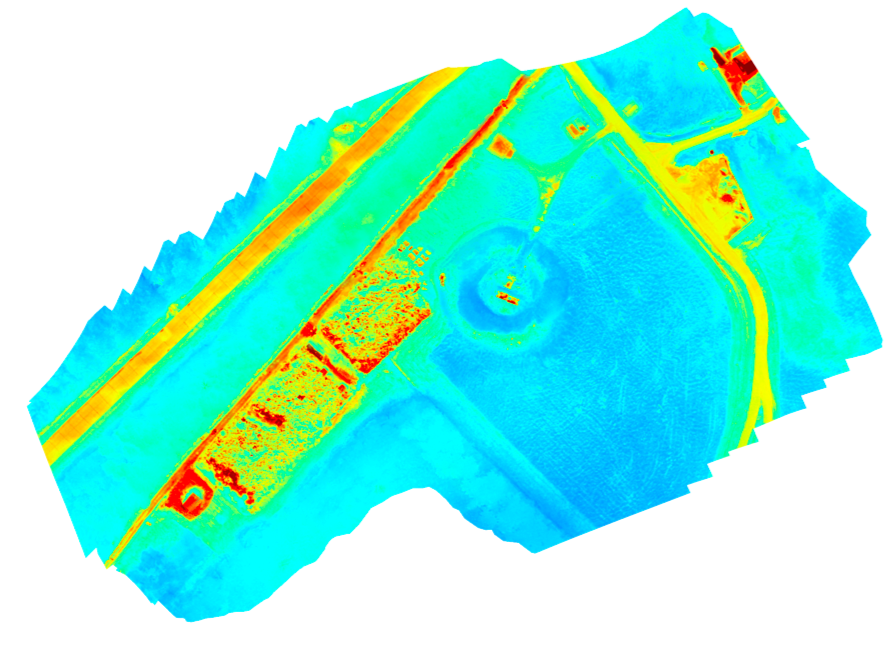
\includegraphics[width=0.9\textwidth]{ROB-15-0035_fig25c.png}
         \caption{FLIR Tau 2 thermal camera}
         \label{fig:ad3}
    \end{subfigure}%
    \begin{subfigure} [b]{0.49\textwidth}
         \centering
         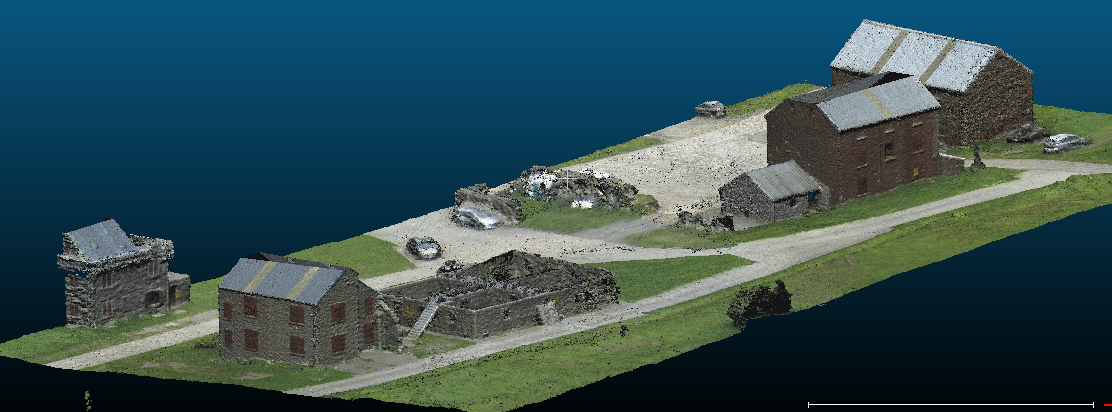
\includegraphics[width=0.9\textwidth]{ROB-15-0035_fig25d.png}
          \caption{Canon IXUS 130 camera in oblique configuration}
         \label{fig:ad4}
    \end{subfigure}%
    \caption{LIFT IV Data.}
    \label{fig:adata}
\end{figure}
\subsubsection{tEODor UGV}
The tEODor was equipped with a laser measurement system based on a rotational LMS 100 sensor.
After semantic 6DSLAM data-collation, this led to the 3D map presented by Figure \ref{fig:tEODorData}.
\begin{figure}
    \centering
    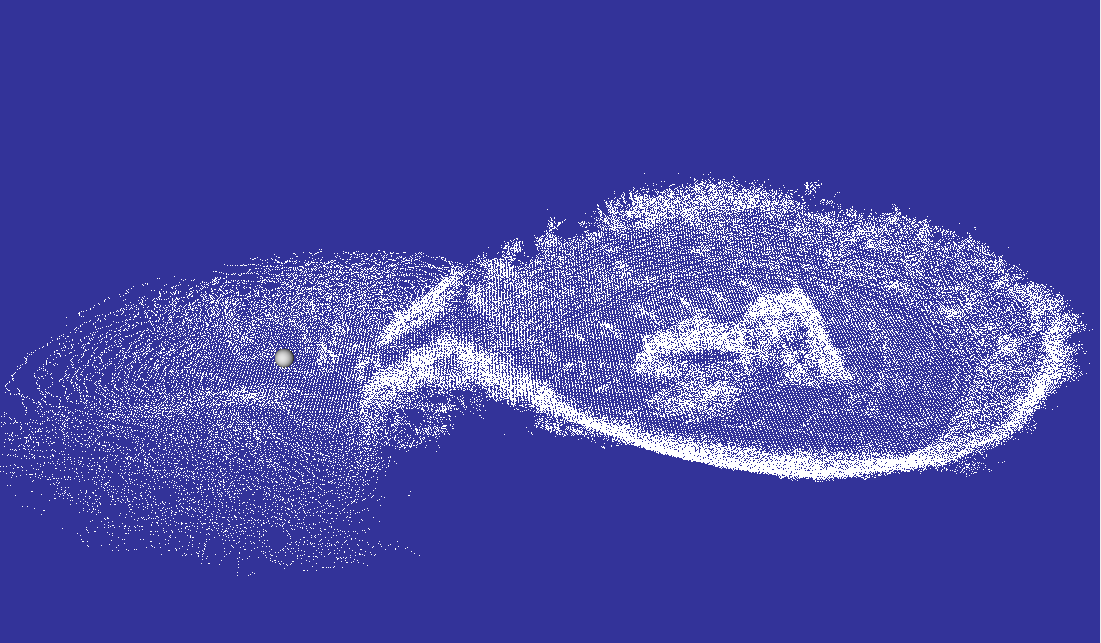
\includegraphics[width=0.7\textwidth]{ROB-15-0035_fig26.png}
    \caption{tEODor Data.}
    \label{fig:tEODorData}
\end{figure}
\subsubsection{ZF 5010 - Husky UGV}
A high-precision geodetic laser system (ZF 5010) was used to gather a detailed 3D map of the area shown on Figure \ref{fig:HuskyData}. Due to the extreme precision and accuracy (1mm) of this dataset, it was used as ground truth for measuring the fidelity of the other measurements. Currently, the Husky robot is combined with the ZF5010 sensor to assemble a versatile inspecting mobile system.

\begin{figure}
    \centering
    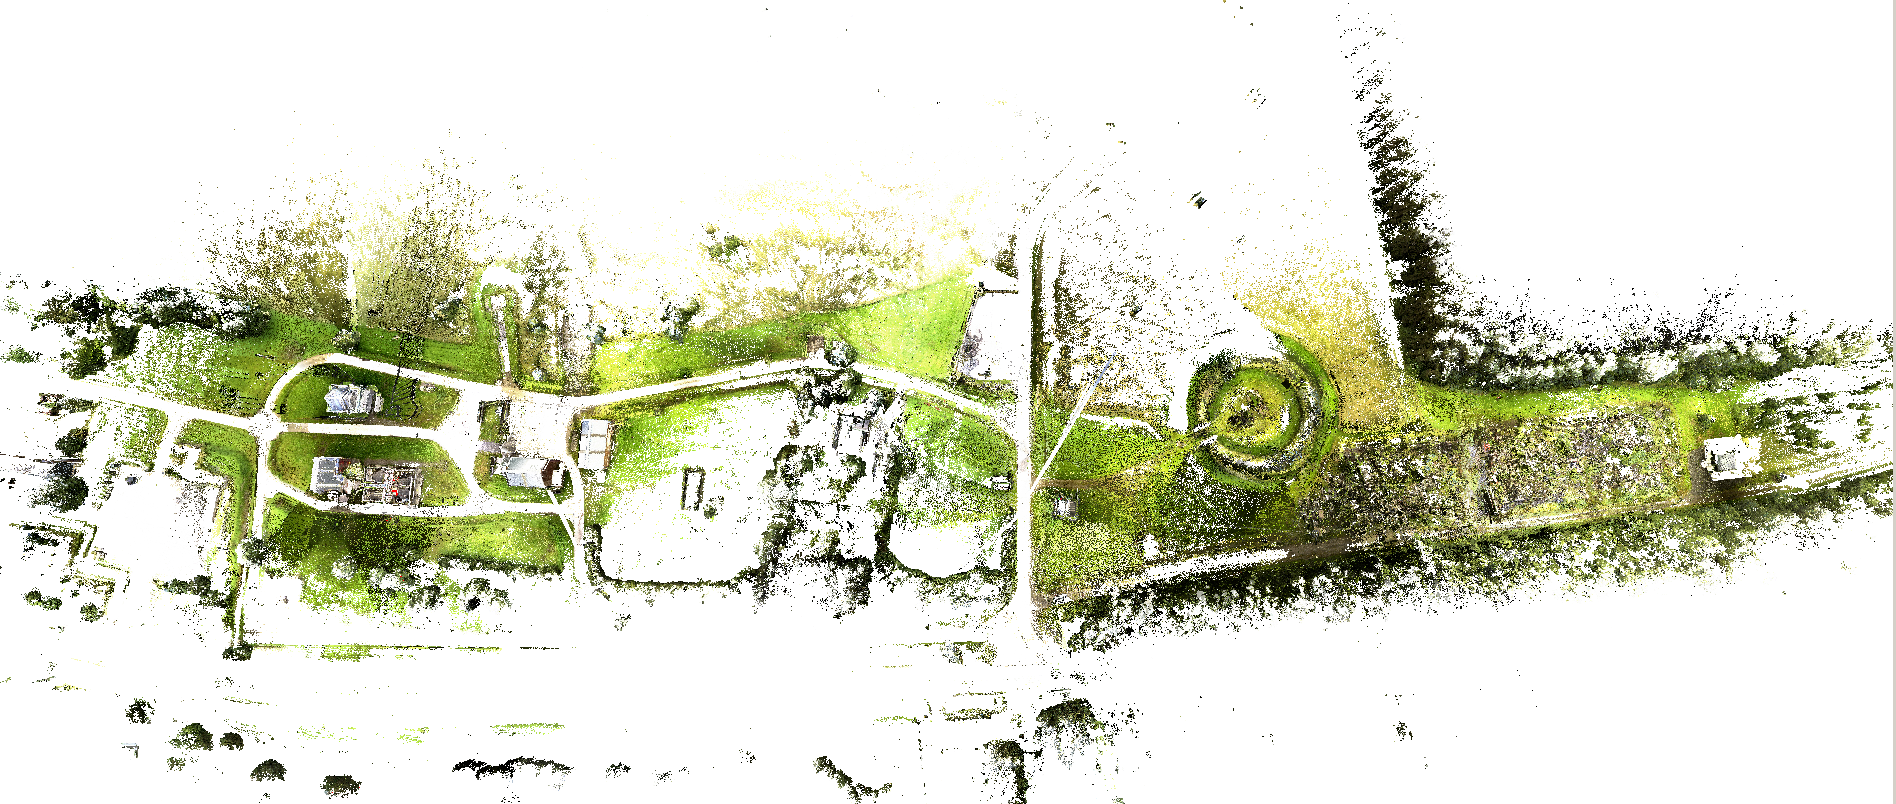
\includegraphics[width=\textwidth]{ROB-15-0035_fig27.png}
    \caption{ZF5010 data - ground truth for the test. }
    \label{fig:HuskyData}
\end{figure}
\subsubsection{Dr-Robot UGV}
The Dr-Robot platform was used for indoor stop-and-scan 3D mapping to demonstrate the advantage of our 3D semantic mapping approach.
To approach real--life challenges in a more accurate way, we included staircases into the scenario.
The platform used here is a lightweight 4-wheel drive robot, which is almost jumping on the stairs.
Therefore, any odometry readings are very poor.
Also, IMU data are very noisy and often saturated.
Described problems are common for typical SAR environments, thus we are confident that data sets gathered with the platform are relevant to real life scenarios.
Figure ~\ref{fig:comparisonLocation1} shows the 3D reconstruction results for both areas using only odometry data.
We observed a problem of merging the ceiling with the floor between levels of the building using classic ICP (the ceiling points are matched with floor points leading to zero-level thickness, as shown in Figures ~\ref{fig:comparisonArea1}a and ~\ref{fig:comparisonArea2}a).
This problem can be solved by a loop closing procedure, but this requires more iterations.
To improve the initial alignment, we propose to use semantic ICP.
Figures ~\ref{fig:comparisonArea1} and ~\ref{fig:comparisonArea2} show a comparison of the results between standard ICP approach and semantic ICP.
Local incorrect floor-ceiling merging initially leads to only small errors, however these errors can drastically change the shape of final point cloud.
Another important issue is the high cognitive load for the human operator trying to perceive proper information from the 3D point clouds.
We introduce the semantic approach, which assigns different colors for ceiling, floor and walls, and therefore can lead to a more intuitively understood map of the environment.
Additionally, the color red is used to mark unstructured objects (e.g. corners, vegetation) in order to assist the detection of areas of interest. The semantic approach to ICP prevents points of different classes from matching, therefore managing to converge faster than classic ICP while also generating a much better starting point for the loop closing procedure.

The loop closing procedure (LUM), which is briefly described in~\cite{Borrmann:2008:GCM:1342428.1342686}, is shown to be able to provide consistent 3D maps but it requires more iterations when calculated for poses that are far from the optimal solution. It is therefore of great importance that the ICP methodology proposed within this paper offers a reliable initial solution. To demonstrate this, we performed a quantitative evaluation of the produced 3D maps by ICP, semantic ICP, LUM and semantic LUM.
This comparison is shown on figure ~\ref{fig:errors}.
Figure ~\ref{fig:errors}a shows histogram of distances of nearest neighbours from reference ground truth data set obtained with geodetic measurement (Z+F IMAGER 5010) and evaluated methods.
It can be observed that the ICP produces the worst 3D map because the number of points with error less than 0.05m is the smallest (54\%), and that the number of points with an error larger than 0.2m is the highest.
To demonstrate quantitatively the problem of floor to ceiling matching we have shown the histogram of angles between normal vectors on figure ~\ref{fig:errors}b.
First, we calculated normal vectors for reference ground truth data and all point clouds of the evaluated methods.
For each point of the cloud created with the use of evaluated methods, we have found the nearest neighbour in the ground truth cloud. For each pair, the angle between normal vectors was calculated.
Ideally, the angle between two matched points should be close to 0.
We can observe a large number of matched nearest neighbours with an angle of more than 160 degrees for the classic ICP method, which demonstrates the problem of floor to ceiling matching (where the normal vector angle difference should theoretically be 180 degrees).
Another interesting observation from figure ~\ref{fig:errors} is that semantic ICP + semantic LUM 10--th iteration is comparable with ICP + LUM 100--th iteration.
We observed that semantic approach gives better performance in the sense of computation time and accuracy. In all cases, the loop closure improves the accuracy of the final maps.

Another important aspect of semantic approach is also that the semantic information is easier to interpret for the user.
Figure ~\ref{fig:fullskier} shows the complete semantic model for the first area along with images of certain areas.
It is easy to distinguish ceilings (blue color), floor, ground (black color), walls (green color) and other objects (red color).
\begin{figure} [h]
	\centering
	\begin{subfigure} [b]{0.4\textwidth}
        \centering
        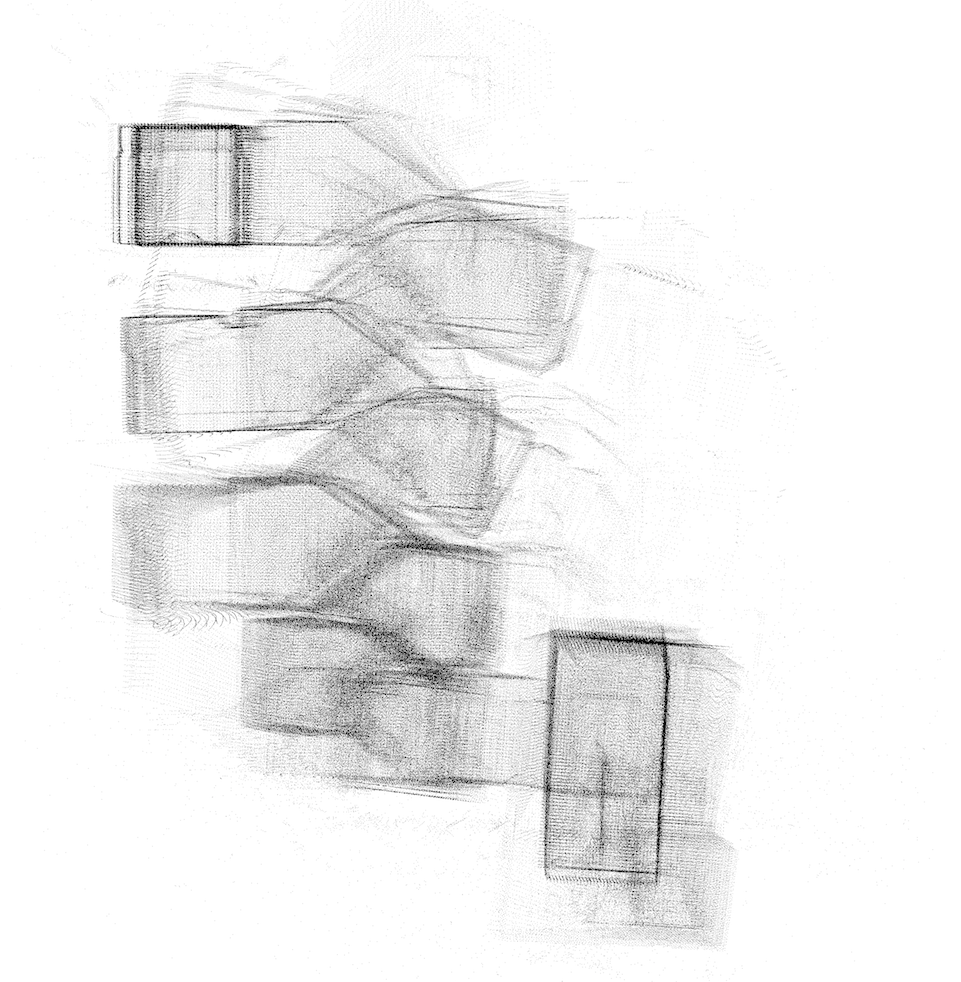
\includegraphics[width=\textwidth]{ROB-15-0035_fig28a.png}
        \caption{Odometry reconstruction of the first site.}
   \end{subfigure}
   \begin{subfigure} [b]{0.59\textwidth}
        \centering
        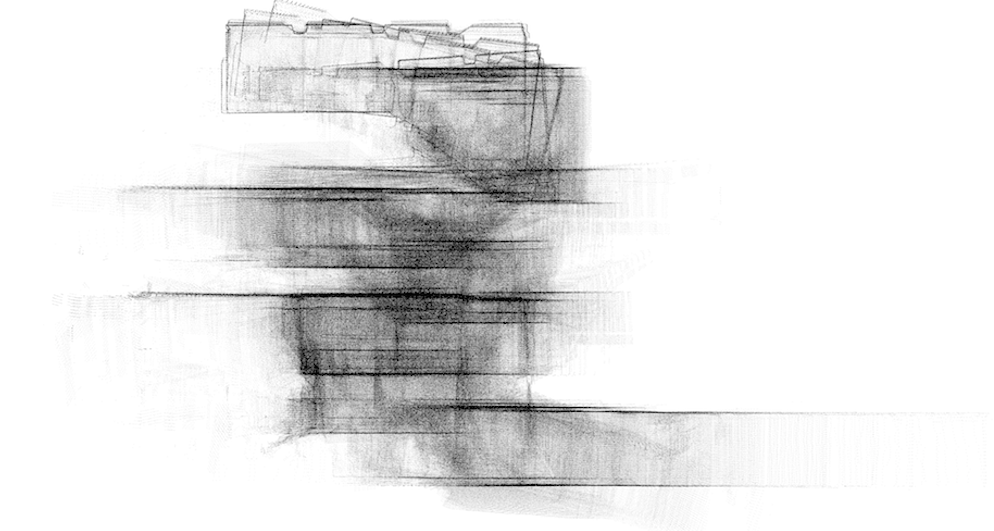
\includegraphics[width=\textwidth]{ROB-15-0035_fig28b.png}
        \caption{Odometry reconstruction of the second site}
   \end{subfigure}
   \caption{3D reconstruction results using odometry data.}
   \label{fig:comparisonLocation1}
\end{figure}
\begin{figure} [h]
	\centering
	\begin{subfigure} [b]{0.49\textwidth}
        \centering
        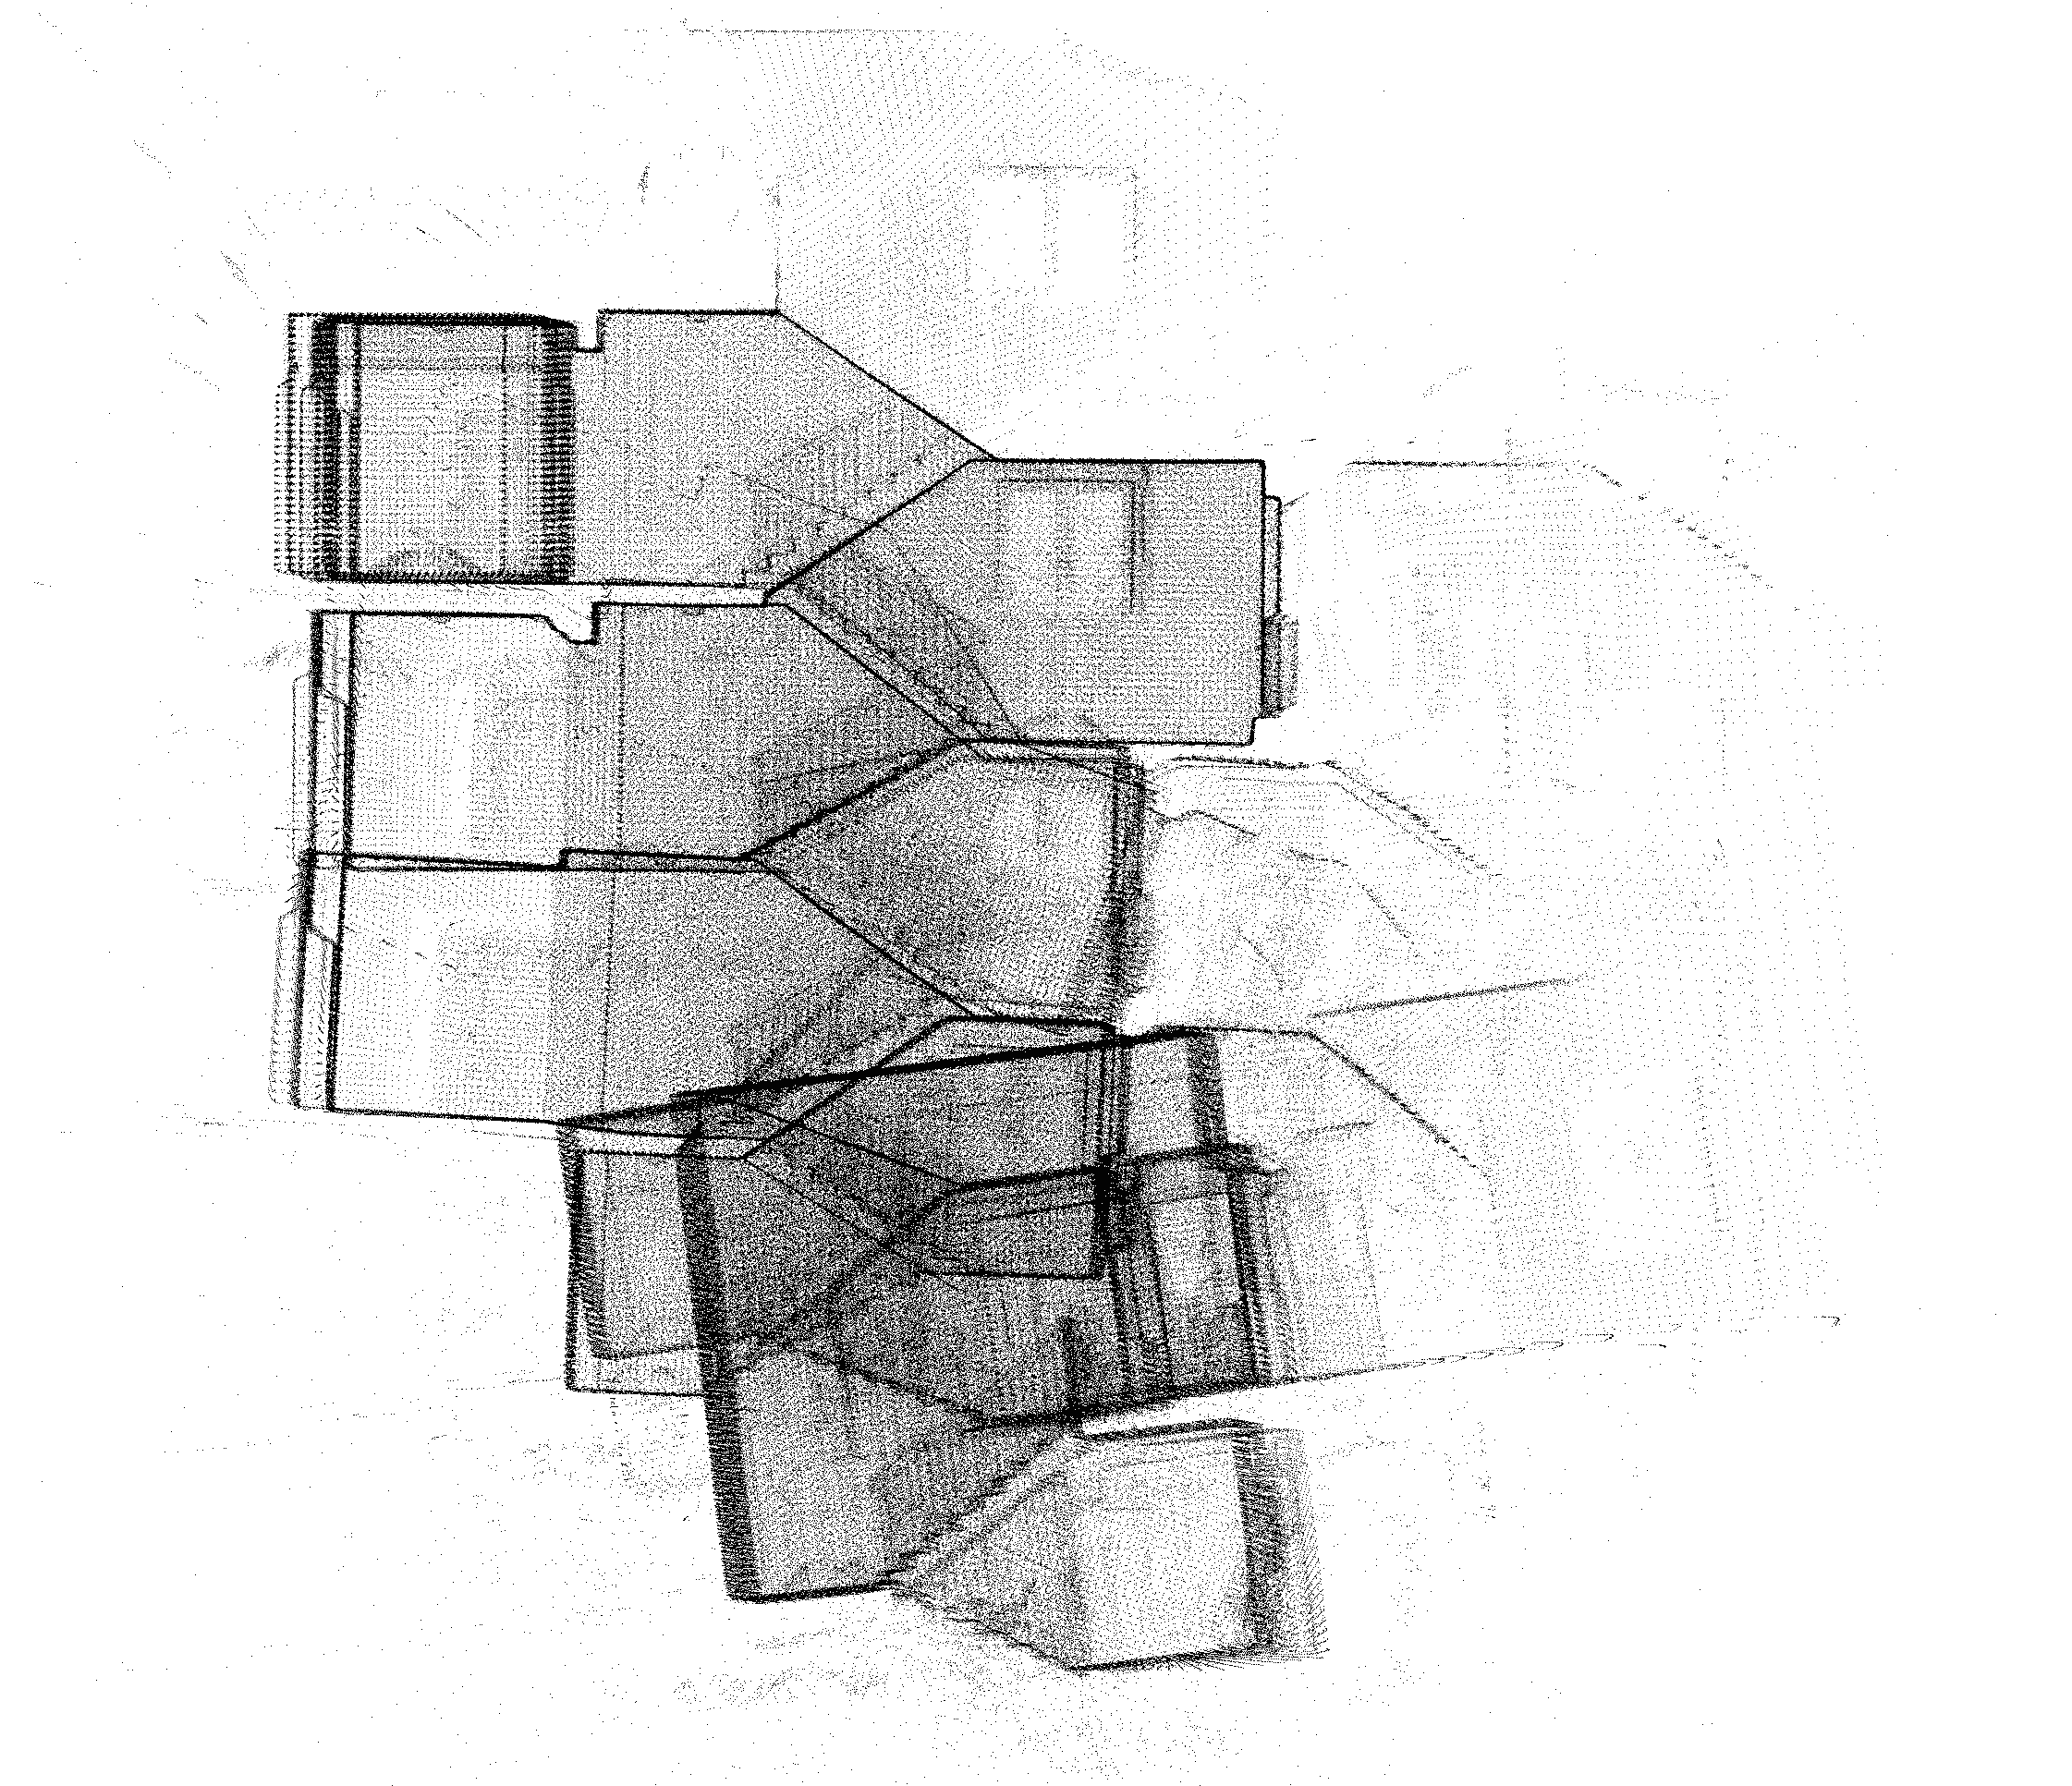
\includegraphics[width=\textwidth]{ROB-15-0035_fig29a.png}
        \caption{Standard ICP reconstruction result}
   \end{subfigure}
   \begin{subfigure} [b]{0.49\textwidth}
        \centering
        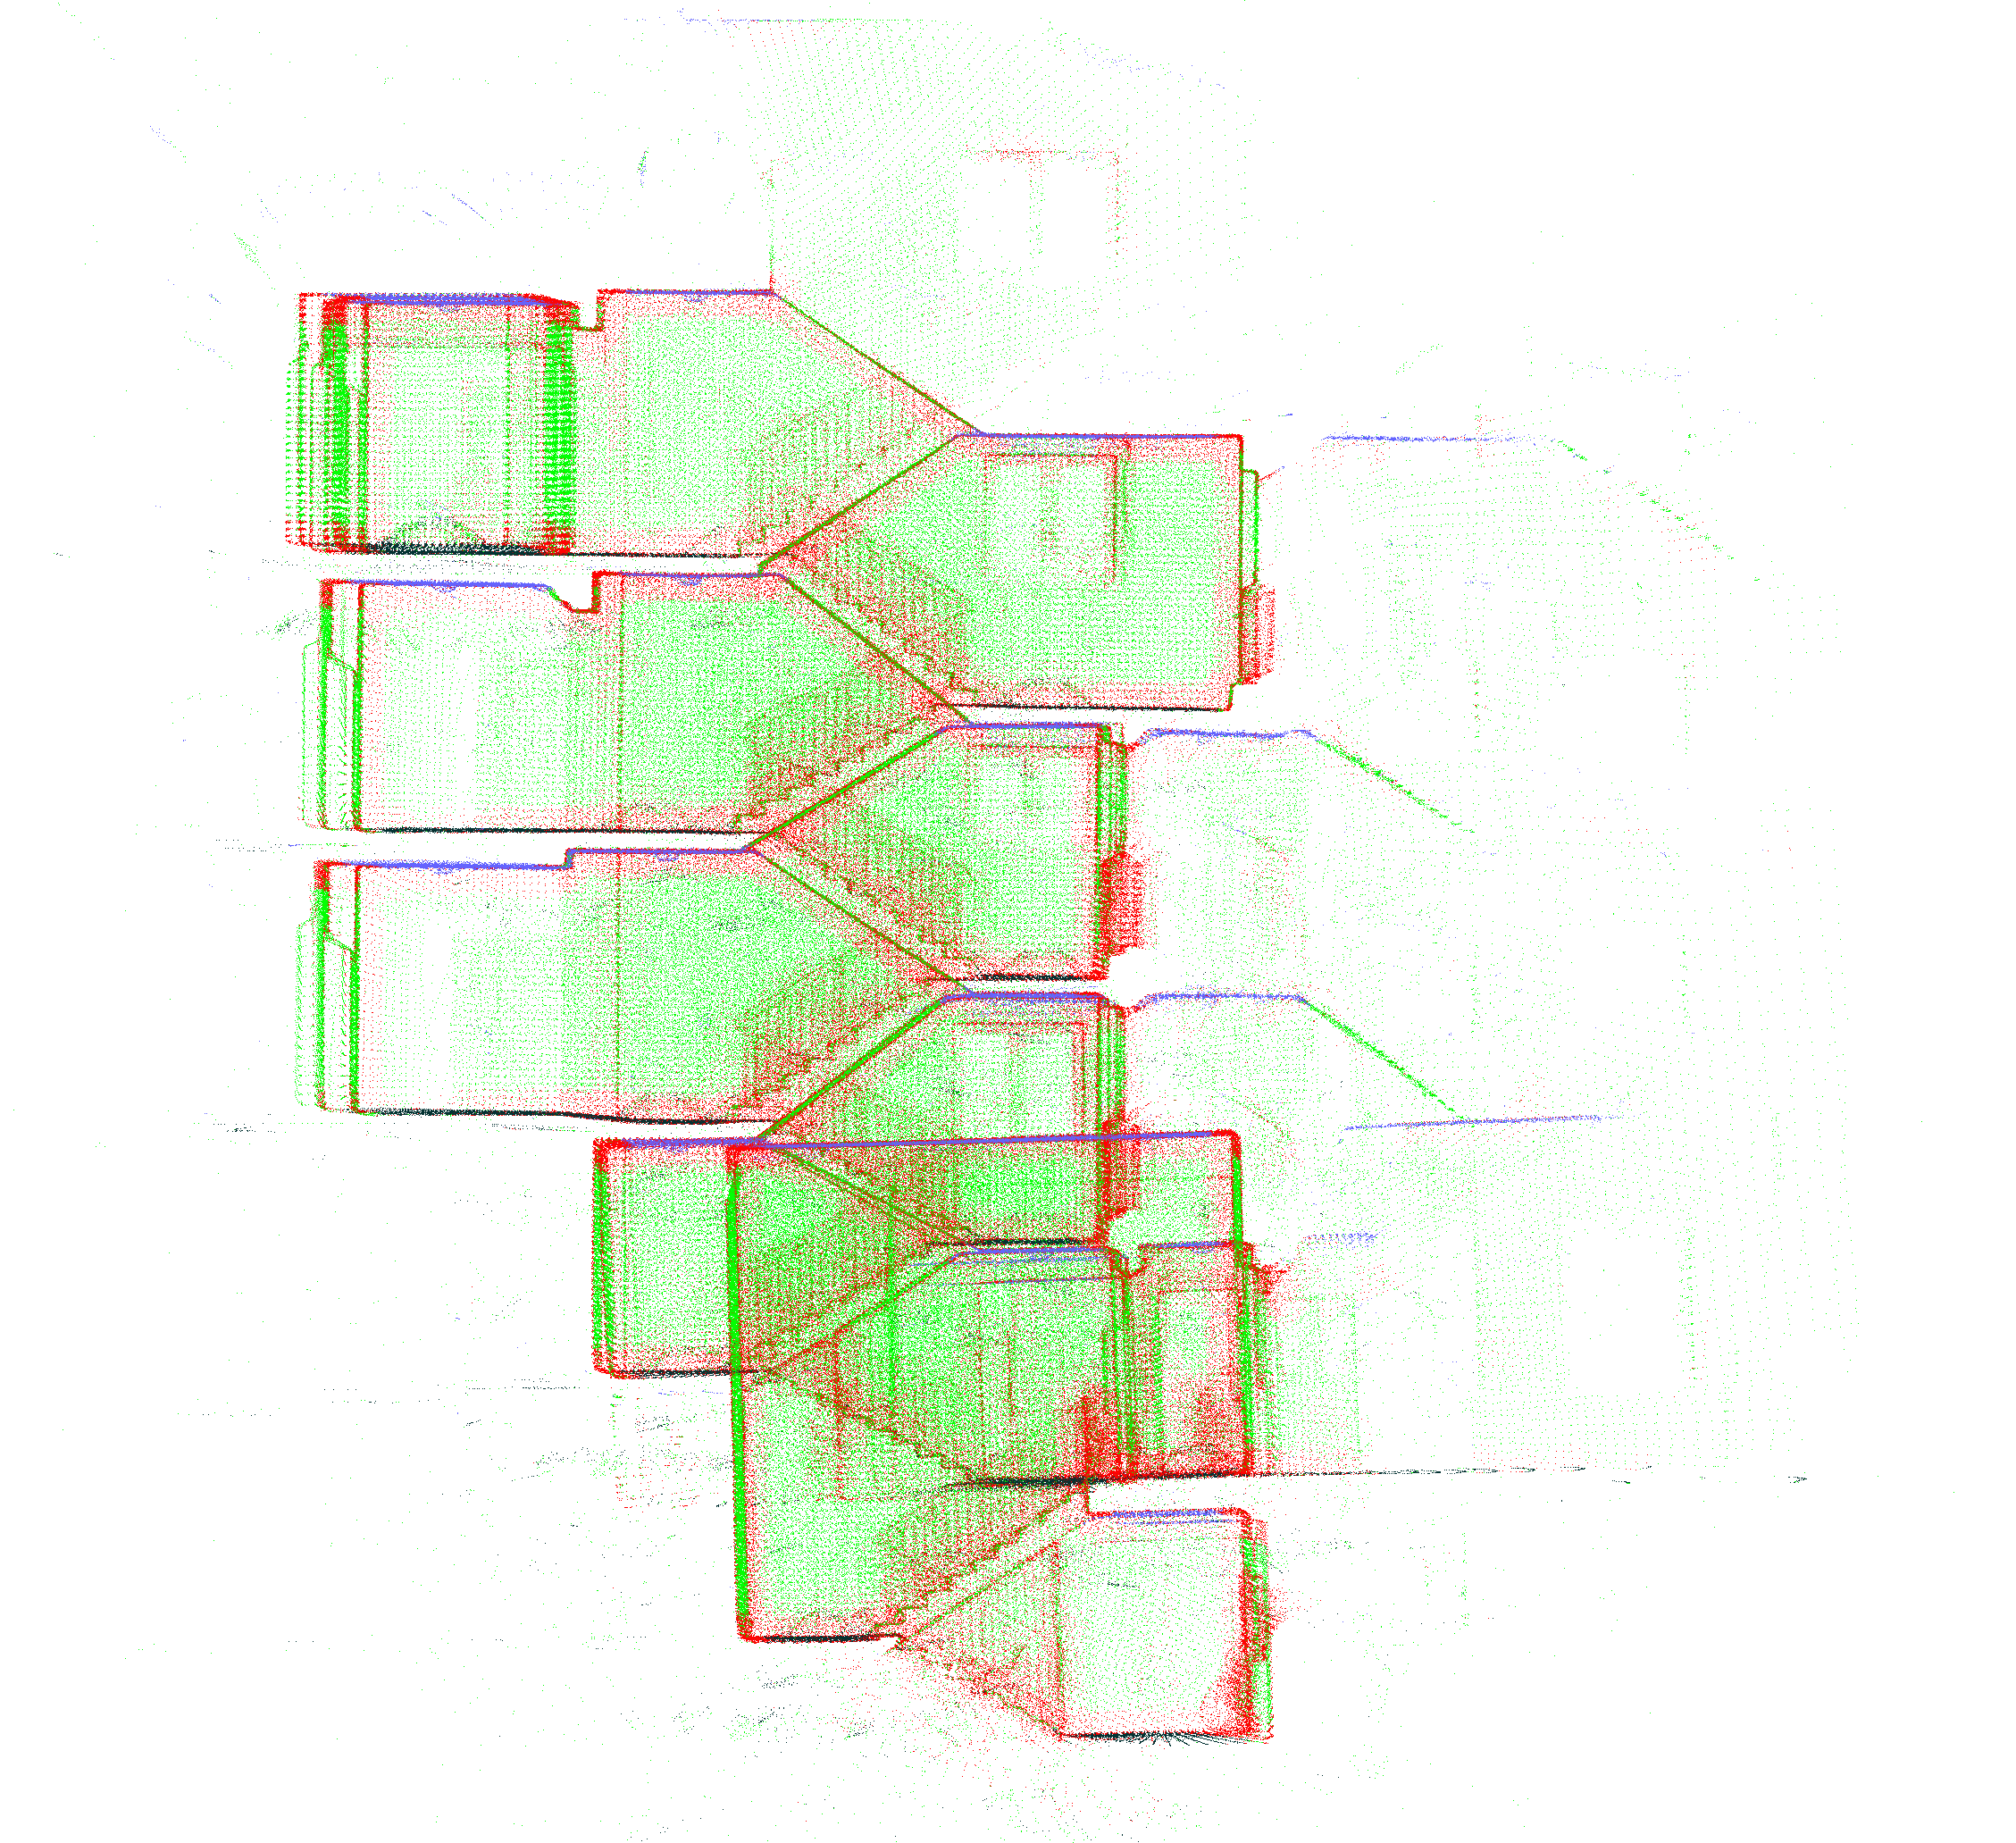
\includegraphics[width=\textwidth]{ROB-15-0035_fig29b.png}
        \caption{Semantic ICP reconstruction results}
   \end{subfigure}
   \caption{The comparison of results between standard ICP approach (left) and semantic ICP (right).}
   \label{fig:comparisonArea1}
\end{figure}
\begin{figure} [h]
	\centering
	\begin{subfigure} [b]{0.49\textwidth}
        \centering
        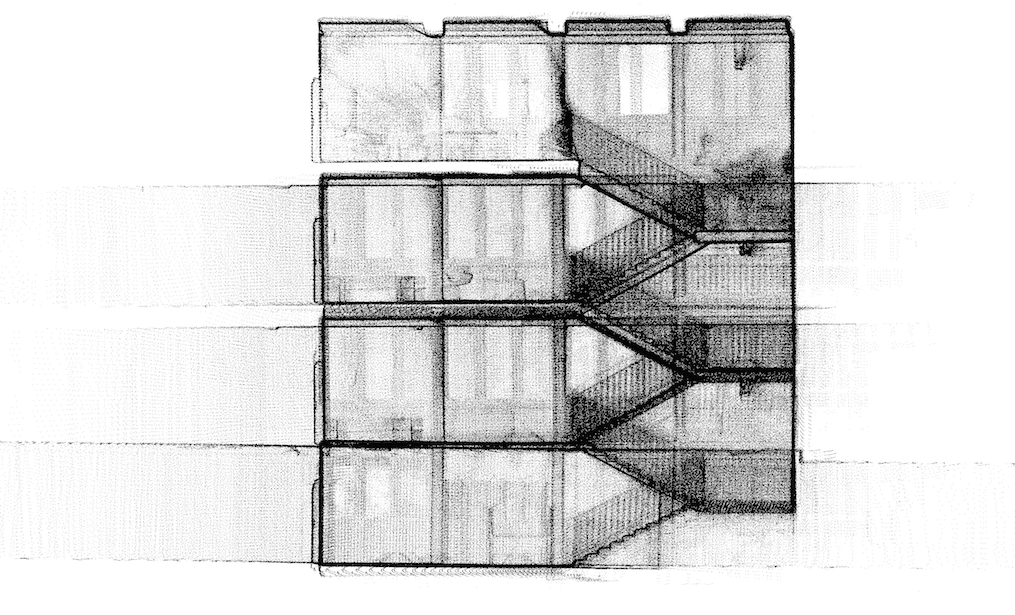
\includegraphics[width=\textwidth]{ROB-15-0035_fig30a.png}
        \caption{Standard ICP reconstruction result}
   \end{subfigure}
   \begin{subfigure} [b]{0.49\textwidth}
        \centering
        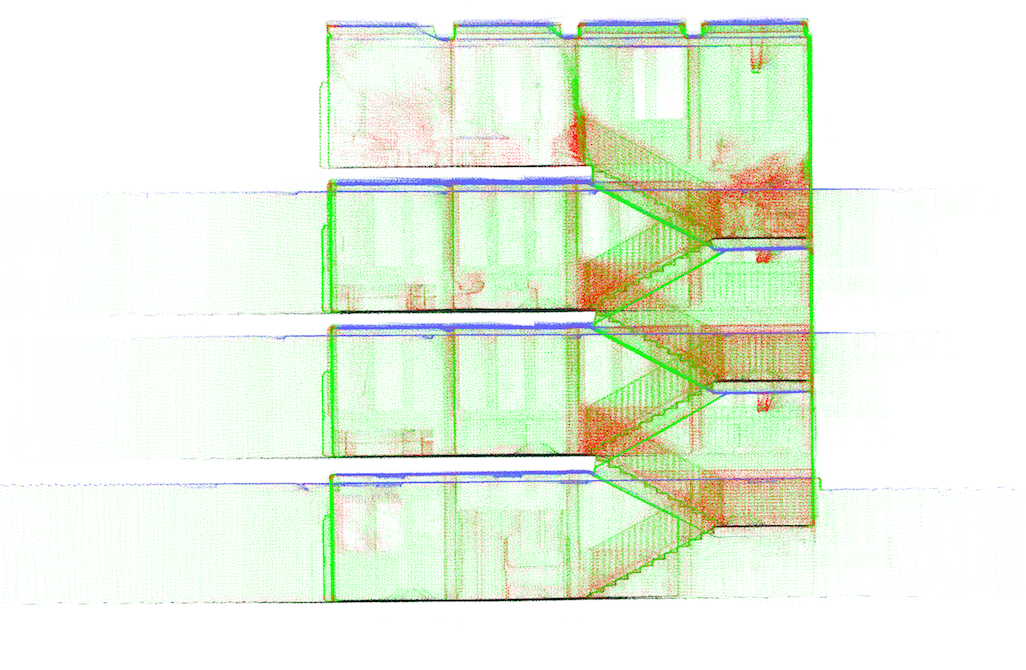
\includegraphics[width=\textwidth]{ROB-15-0035_fig30b.png}
        \caption{Semantic ICP reconstruction results}
   \end{subfigure}
   \caption{The comparison of results between standard ICP approach (left) and semantic ICP (right).}
   \label{fig:comparisonArea2}
\end{figure}

\begin{figure}
\centering
 \begin{subfigure} [b]{0.49\textwidth}
         \centering
         \includegraphics[width=\textwidth]{ROB-15-0035_fig31a.png}
         \caption{Histogram of distance error for pairs}
    \end{subfigure}
   \begin{subfigure} [b]{0.49\textwidth}
         \centering
         \includegraphics[width=\textwidth]{ROB-15-0035_fig31b.png}
         \caption{Histogram of angle difference for pairs.}
    \end{subfigure}
\caption{Quantitative evaluation of 3D mapping methods.
ICP performs worst - only 55\% of points with error less than 0.05m and 6\% of points with the angle between normal vectors more than 170 degrees (matching floor to ceiling problem).}
\label{fig:errors}
\end{figure}

\begin{figure}
 \centering
    \includegraphics[width=\textwidth]{ROB-15-0035_fig32.png}
    \caption{Complete semantic model of the first area, it is possible to distinguish ceiling (blue color), floor, ground (black color), walls (green color) and other objects (red color).}
    \label{fig:fullskier}
\end{figure}
\clearpage
\subsection{Data Fusion \& Rendering}
The UAV and UGV systems described above were used to create a multi-layer map of an abandoned village on the terrain of Camp Roi Albert, in Marche--en--Famenne, Belgium. The mapped area of size approximately 600mx400m, was chosen because of its resemblance to a SAR environment. Table ~\ref{table:sourcesMEF} shows different sources of 3D point clouds used by the system along with their platforms. For each system a measure of approximate average accuracy was given.
For laser systems, this is the accuracy of the laser range scanner.
The UAVs are equipped with cameras, so 3D point clouds are generated from pictures.
The accuracy measure was calculated based on the error of image matching (in pixels) against Ground Control Points marked with differential GPS and the resolution of pixels for the horizontal and the vertical axis. All point clouds were merged together using the approach described in previous subsection (initial placement by operator and detailed matching using semICP algorithm).
The data gathered using the ZF 5010 laser system (figure \ref{fig:HuskyData}.) were matched separately using geodetic methods and are used as ground truth for other measurements.
The results of the matching are shown in the last column of the table.
Matching accuracy was calculated as a weighted mean value from histograms gathered as described in section 6.3.6.

\begin{table}[h!]
\centering
\begin{tabular}{| c | c | p{3cm} | p{2cm} | p{2cm} |}
\hline
Platform & Sensor Description & Measurement Accuracy & Matching Accuracy\\
\hline
AtlantikSolar & Aptina MT9V034 & 15.2cm (horizontal); 16.0cm (vertical) &186cm\\ \hline
AtlantikSolar & Sony HDR-AS100VW GPS-tagged & 18.0cm (horizontal); 30.0cm (vertical) &  136cm \\ \hline
MD4-1000 & Sony Nex Alpha & 2.0cm (horizontal) &125cm\\ \hline
LIFT IV & Canon IXUS 130 & 1.1cm(horizontal); 118.4cm(vertical) &129cm\\
LIFT IV & Aptina MT9V034 & 3.0cm(horizontal); 21.5cm(vertical) &92.6cm\\
LIFT IV & FLIR Tau 2 & 5.0cm(horizontal); 34.0cm(vertical) &131cm\\ \hline
tEODor & LMS 100 Laser system & 3cm &6.76cm\\ \hline
Dr-Robot & LMS 100 Laser system & 3cm &6.76cm\\ \hline
Husky & ZF 5010 Laser system & 1mm & na\\ \hline
\end{tabular}
\caption{Details of data gathering platforms}
\label{table:sourcesMEF}
\end{table}
As a qualitative analysis, we tested merging data from the multiple independent robotic systems described above.
The UAVs were used for image data collection and DTM-generation (DTM is shown on figure ~\ref{fig:MeFuav}).
The UGVs were used for collecting detailed 3D data of chosen areas of interest, including an indoor exploration of 3 buildings.
The resulting map is shown on figure ~\ref{fig:MeFugv1}.
The idea is that operators collect data using the robots and then transfer it to the mobile data center.
Once all data are in storage in the Cloud, these maps are matched into a common environment model.
The matching is done in a semi-autonomous fashion.
Although ICP is quite resistant to positioning errors of matched point clouds, as previously shown in the paper, a rough initial position estimate is required.
The ground vehicle odometry system provides initial positioning accurate enough to match results for their sensor systems.
However the global positioning between aerial scans and ground scans is missing.
Because of that the operator has to provide initial positioning between aerial and ground models. After that the precise matching is done by ICP.
The matching is possible because aerial and ground scans can be transformed to common form by proper use of sub-sampling (for compatible density) and semantic classification (for finding areas of similar characteristics).
The result is shown on figure ~\ref{fig:MeFuav+ugv}, with a zoomed view on figure ~\ref{fig:MeFuav+ugvZoom1}.
Using the mobile data center allows to reduce computation time as the operator can have full hardware support for the taks of performing 6D-SLAM.
Another important functionality of the Cloud system is that all renders shown in figure ~\ref{fig:datafusion} are available in a SaaS model via XenApp for all users involved in the SAR mission.
This provides the team with a real-time parallel access to all data already put in the data center.
The ortho-mosaic generated by post--processing data from the mapping mission can be accessed from the Cloud, configured as a layer in the Geographical Information System (GIS) and rendered in the C2I over the existing base map layer, as seen in figure~\ref{fig:c2i_ortho_UAVs}.
Data visualization was tested with 10 clients working concurrently on the server.
Figure ~\ref{fig:networkstats} shows network usage during the experiments.
The test was conducted in two phases: with 5 users following by extension to 10 users.
The maximal average network usage was 4.2 Mbit/s.
The peak values were 2.4 Mbit/s for 5 users and 5.3 Mbit/s for 10 users. Both of those values are far below the maximal local network capability (theoretical value of 1Gbit/s).
An important aspect is that, even though the computers used as client had low configuration (Intel Celeron 2,80 GHz CPU with 1 GB of ram), the rendering and work with applications was smooth.
\begin{figure} [h]
	\centering
	\includegraphics[width=0.75\textwidth]{ROB-15-0035_fig33.png}
	\caption{Network usage for 10 users of data visualization.}
	\label{fig:networkstats}
\end{figure}
\begin{figure} [h]
    \centering
    \begin{subfigure} [b]{0.45\textwidth}
         \centering
         \includegraphics[scale=0.552]{ROB-15-0035_fig34a.png}
         \caption{3D map from UAVs}
         \label{fig:MeFuav}
    \end{subfigure}%
    \begin{subfigure} [b]{0.45\textwidth}
         \centering
         \includegraphics[scale=0.2532]{ROB-15-0035_fig34b.png}
         \caption{3D map from UGVs}
         \label{fig:MeFugv1}
    \end{subfigure}
    \begin{subfigure} [b]{0.45\textwidth}
         \centering
         \includegraphics[scale=0.459]{ROB-15-0035_fig34c.png}
         \caption{Fused 3D map}
         \label{fig:MeFuav+ugv}
    \end{subfigure}%
    \begin{subfigure} [b]{0.45\textwidth}
         \centering
         \includegraphics[scale=0.55]{ROB-15-0035_fig34d.png}
         \caption{Zoomed fused 3D map}
         \label{fig:MeFuav+ugvZoom1}
    \end{subfigure}%
    \caption{Data fusion from 3D mapping systems.}
    \label{fig:datafusion}
\end{figure}

\begin{figure}
 \centering
    \includegraphics[scale=0.4]{ROB-15-0035_fig35.png}
    \caption{Ortho-mosaic from the cloud configured as a base layer in the C2I.}
    \label{fig:c2i_ortho_UAVs}
\end{figure}
Out of the discussion with end-users present at the trials, it was concluded that the merged UAV and UGV data are very useful for SAR operations.
The 3D laser system from a ground mobile robot can bring additional local information for extending global operational awareness.
By combining aerial and ground mapping we obtained a satisfactory solution for SAR mapping. The data sets gathered during the experiment are from following address: http://projects.asl.ethz.ch/datasets/doku.php?id=jfricarus .

\subsection{Use of gathered data for SAR training}

Remote training of the robot operator was carried out using the C2I as a client in Belgium connected to the remote data center hosting the SAR simulator in Poland.
Figure~\ref{fig:c2i_IMMSim_cam} shows a screenshot of the C2I rendering virtual robot sensors such as virtual camera views, GPS and Inertial data.
The SAR training tools explained in section 5 were deployed using the high-performance computing architecture presented in section 4.
The base for the tools is Vortex rigid body engine capable of simulating rigid dynamics, cables and deformable soil.
For the rendering purpose we are using OpenSceneGraph (OSG).
Together these frameworks are sufficient enough to provide high-fidelity simulation.
Users can connect to the training applications (camera view, virtual joystick) in XenApp models or run them from a VDI.
As client applications are not using the GPU for computation, the main drawback of VDI is not applicable.
The training tools are dedicated for an e-learning procedure before training on real hardware (robot, RC2). The use of a local Cloud allows to run the tools on any computer within the network of the server.
If the server is connected to the Internet the tools are available on-line.
The same applications may be used in the Mobile Data Centre.
The goal of these tools is to introduce robotic hardware to end-users with the minimization of cost, effort and installation problems related with the costly licensing.
To increase the fidelity of virtual training, we decided to use the UAV 3D data from the experiment, shown on figure ~\ref{fig:datafusion}, for building a 3D model of the environment.
A virtual representation of the environment, with three virtual Large Unmanned Vehicles UGVs, is shown on figure ~\ref{fig:training}.
Currently, a single server can perform efficient simulation of 10  LUGVs and SUGV's.
Network usage for 10 users was 1.4 Mbit/s with two cameras per users.
The Mobile Data Centre is scalable, therefore it can be easily extended for even more systems.
\begin{figure}
    \centering
    \includegraphics[width=0.9\textwidth]{ROB-15-0035_fig36.png}
    \caption{Virtual sensor data from the simulator to C2I.}
    \label{fig:c2i_IMMSim_cam}
\end{figure}

\begin{figure} [h]
    \centering
    \begin{subfigure} [b]{0.33\textwidth}
         \centering
         \includegraphics[scale=0.5]{ROB-15-0035_fig37a.png}
         \caption{Virtual training environment.}
         \label{fig:map}
    \end{subfigure}
    \begin{subfigure} [b]{0.33\textwidth}
         \centering
         \includegraphics[scale=0.52]{ROB-15-0035_fig37b.png}
         \caption{3 LUGVs.}
         \label{fig:LUGV3}
    \end{subfigure}
    \begin{subfigure} [b]{0.33\textwidth}
         \centering
         \includegraphics[scale=0.5]{ROB-15-0035_fig37c.png}
         \caption{View from camera of LUGV.}
         \label{fig:LUGV2}
    \end{subfigure}
    \caption{SAR training tools in SaaS model.}
    \label{fig:training}
\end{figure}

\afterpage{\clearpage}

\subsection{Discussion and future improvements}


	A noticeable drawback of the system is lack of robust positioning solution for connecting data gathered by UAVs and UGVs. In the future we plan to increase positioning accuracy of individual systems and integrate them into a common reference.
	
	
	During the work on the system we noticed a potential for integrating additional data source into the global map.
Currently we are working on improving the UGV's sensor equipment to increase their usefulness.
By adding a high resolution pan-tilt camera we equip the Husky robot with the capability of gathering spherical images of given area.
The initial results are shown on figure ~\ref{fig:streetview}.
We also plan on adding autonomous outdoor capabilities to the ground platforms.
Autonomous navigation would be done based on maps initially gathered by the UAVs.
The main idea is to give the SAR personnel the possibility to create a complex data documentation of given area on demand.
	
	
	We see a possibility of increasing the accuracy of the 6D-SLAM algorithm.
	After analyzing the results and the current state of the art we concluded that in this area we are close to the limits provided by the ICP method.
	As such, future work will concentrate on finding and testing different approaches to the subject.

\section{Operational Validation}
\subsection{Situational Overview}
In the period between end of May and beginning of June 2014, Bosnia and Herzegovina and Serbia were hit hard by catastrophic massive flooding after abundant rainfall over a couple of few weeks causing floods and landslides.
The countries suffered great damage, as the rain was the heaviest in 120 years of recorded weather measurements.
Only in Bosnia and Herzegovina, an estimated 1.5 million people were affected (39\% of the population). Flooding has led to at least 53 deaths in both countries \cite{bosnia}.
The  EU  Civil  Protection  Mechanism  was  activated  due  to  the catastrophic crisis and 22 EU Member States offered assistance through the Mechanism.
Figure \ref{fig:bosna} shows the flood situation (26 May 2014) and the deployment of international teams through the EU Civil Protection Mechanism.
The whole northern and partially central region of the country were heavily affected and - based on \cite{bosnia} - the relief efforts were hampered by the destroyed infrastructure, broken telecommunications, blackouts, etc.
\begin{figure}
    \centering
    \includegraphics[width=0.9\textwidth]{ROB-15-0035_fig38}
    \caption{Bosnia flood map (source: EU Commission).}
    \label{fig:bosna}
\end{figure}

To make matters worse, the presence of many Explosive Remnants of War (ERW) remaining from the Balkan Civil War of the nineties, created an extremely dangerous situation for the local population and the relief workers. The natural disaster with the floods, torrents, landslides, land shifting had an intensive destructive impact on suspected hazardous areas (SHA) and minefields in Bosnia and Herzegovina. Only in Bosnia and Herzegovina, $831.4 km^2$ were flooded, $37.48 km^2$ of suspected hazardous area in 33 areas were under direct impact of torrents and landslides; by the 4th of July 2014, 1018 pieces of unexploded ordnance, 92 mines and 3 cluster bombs were found, as well as 40.163 ammunition pieces.
In addition, $80.2 km^2$ of new areas which previously had not been mine suspected became potentially hazardous (Northern part  of  Bosnia and Herzegovina).
The Bosnian Mine Action Centre (BHMAC) provided data and information about the affected regions, the kinds of influence, the impact intensity and the spatial distribution, as well as the priorities \cite{bosnia2}.
The problem of shifting minefields also hampered the provision of aid and relief and debris clearance.

\subsection{Bosnian relief mission}
Among many other international SAR teams, the Belgian First Aid and Support Team (B-FAST) zqs deployed to Bosnia to help with relief operations.
Along with the B-FAST team, the Belgian Royal Military Academy sent the first author of this paper and the Unmanned Aerial Vehicle discussed in section 6.2, together with 3D mapping tools, in order to assist the teams for task such as damage assessment, dike breach detection, mapping, aerial inspection and for re-localizing the many explosive remnants of war (ERW) which have been displaced due to the landslides \cite{bosnia1}. The cloud computing and data management tools described in sections 4 and 3 were deployed in order to give the end users access to the data gathered by the unmanned system. This mission fits in the framework of the European research projects ICARUS \cite{ICARUS} and TIRAMISU (on humanitarian demining) \cite{tiramisu}.

On the field, we assisted a team of the Bosnian Mine Action Centre (BHMAC) which was deployed to multiple regions of the country in order to localize the displaced ERW.
In the first critical phase we have provided to BHMAC the support to urgent actions (urgent demining, assessment of status of minefields) by aerial survey.

Flight permits up to a flight altitude ceiling of 150m for the complete Bosnian territory were granted with the support of the Ministry of Security of Bosnia and Herzegovina and the national Directorate of Civil Aviation (BHDCA).
Due to the crisis situation and thanks to the fact that all application documents for the flight permits were readily available (as they were already prepared for the Marche—en--Famenne trials), these flight permits were issued within half a day after a coordination meeting in the capital Sarajevo with the Bosnian Ministry of Security.
In a period of two weeks, we operated with a Vertical Take-Off and Landing Remotely Piloted Aircraft System on 13 locations (in the north and central part of the country).
We performed around 20 flights within Visual Line of Sight in urban and semi-urban areas. In general, two types of operations were performed:
\begin{itemize}
\item \emph{Manual Flights}. End-users (rescue or demining teams) indicated points of interest they wanted to see investigated by the UAV, mainly for damage assessment and visual inspection.
The flights were then executed by a trained operator.
\item  \emph{Waypoint-based mapping flights}. An area to be mapped by the UAV was indicated by the end-users. A flight plan was then set up to map this area using an autonomous waypoint-based flight.
Also under these conditions, a trained pilot always operated the remote control station.
\end{itemize}

A typical flight had a duration of 25 to 30 minutes, which enables to cover an area of about 1 hectare. Multiple mapping missions were performed, gathering 200 to maximum 500 images with a resolution of 24 megapixels and mapping areas as large as $1km^2$.

\subsection{UAS deployment for relief operations support}
One of the cities which was hit most by the floods was the city of Orasje (located north-east) where B-FAST was deployed.
The UAV was first deployed here to assist the B-FAST team for assessing the optimal location to install their high-pressure pumps and to monitor the water levels, as shown on Figure \ref{fig:UASp1} to \ref{fig:UASp1b}.
The problem with the installation of the water pumping system was that water levels were not decreasing after multiple days of pumping, due to an undetected dike breach.
The ICARUS-TIRAMISU UAS was able to locate this broken dam, as shown on Figure \ref{fig:UASp2}.
Expert analysis indicated that this dam breach could not have been caused by natural means, so the Bosnian Ministry of Justice has started a justice case against the individual(s) who may have caused it and commissioned the ICARUS-TIRAMISU UAV image material as evidence.
The UAS proved very useful in support here to quickly detect dike breaches and to map the area quickly. Landing on dry land was a challenge, however, as there were virtually no spots of clear and open land suited for takeoff and landing.
As a result, all takeoff and landing operations were done on remote control by a trained pilot.

\begin{figure}{
\centering
 \begin{subfigure}[t]{0.49\textwidth}    \centering          \includegraphics[width=0.9\textwidth]{ROB-15-0035_fig39a}      	\caption{Flooded City of Orasje}                	\label{fig:UASp1}       	\end{subfigure}
\begin{subfigure}[t]{0.49\textwidth}       \centering       \includegraphics[width=0.9\textwidth]{ROB-15-0035_fig39b}      	\caption{UAS used for the operations}                	\label{fig:UASp1is}       	\end{subfigure}
 \begin{subfigure}[t]{0.49\textwidth}       \centering       \includegraphics[width=0.9\textwidth]{ROB-15-0035_fig39c}      	\caption{Optimization of the location for the B-FAST water pumps}             \label{fig:UASp1b}       	\end{subfigure}
 \begin{subfigure} [t]{0.49\textwidth} 		\centering \includegraphics[width=0.9\textwidth]{ROB-15-0035_fig39d}      		\caption{Broken dam on the Sava river detected by the UAS}	\label{fig:UASp2}  		\end{subfigure}
\caption{UAS used for relief operations support.}
\label{fig:bpicall}}
\end{figure}


Next to the operations in support of the B-FAST team, the UAS was also deployed on request of the German Federal Agency for Technical Relief team and Austrian relief workers working on the incident site.
These teams asked for assistance of our UAV system for aerial inspection, damage analysis and improving their situation awareness and for selecting the optimal location for the installation of the high-pressure water pumps.
The Ministry of Security and the Federal Civil Protection of Bosnia and Herzegovina also asked for UAV aerial support in the region of Kopanice (Southeast of Orasje), where the flood waters from Sava River broke the dams.
The flood waters  flowed through these breaches and completely submerged the agricultural lands and all the people needed to be evacuated.
This mission was especially risky because the location of the broken dam area was in a mine suspected region.
During the mission, we often faced the problem to get around from one place to another, as this was very difficult due to the damaged infrastructure (see Figure \ref{fig:UASp3}).

\subsection{UAS deployment for demining operations support}
Bosnia and Herzegovina was contaminated with land mines due to the war from $1992$ to $1995$ and as a result the country has one of the most serious land mine problems in the world.
One of the cities which was hit hard by the floods was the city of Maglaj, as shown on figure \ref{fig:UASp4}. An additional problem in this region was the presence of many ERW, rendering the deployment and work of the relief teams extremely dangerous.
As a result, it was decided to deploy the UAV system for inspection flights, especially into areas where the relief teams could not access due to the high risks.
The UAV was used for aerial assessment and mapping of the mine-suspected areas and to find indicators of where the minefields were shifted due to the floods and landslides.
Figure  \ref{fig:UASp5} shows a re-allocated minefield due to landslides.
The data of the UAV was mostly important in assessing the ground movement due to  landslides.
Figure \ref{fig:frmap} shows the first post-processing results of the region Olovo-Olovske Luke (central Bosnia and Herzegovina).
The UAV was used for providing 3D-maps, ortho-photos and DEM of the environment to analyze the effects of the landslides on mines and ERW.
This results has been used as initial models by BHMAC for spatial estimation of new hazardous risk caused by the shifting of landmines and unexploded ordnance (UXO) to wider areas which had not been mine suspected before the disaster.
Fusing the obtained data from the UAV (3D Digital Terrain Models) with pre-existing data (mine risk maps from satellite imaging and the Mine Action Centers), it was possible to predict the movement of the landmines and to generate updated mine risk maps and maps of mine-affected areas.
To give an indication of the scale of the problem, it can be reported that mines were found up to $23$ kilometers from their original location.
This means that the search area is huge and that the effectiveness of area reduction techniques like the use of the UAV, combined with 3D mapping predicting the ERW-movement and thereby limiting the search area, can be dramatic. More information about this mission can be found in \cite{BosniaUAS}.

\begin{figure}
\centering
 \begin{subfigure} [b]{0.49\textwidth}     \centering     	\includegraphics[width=0.9\textwidth]{ROB-15-0035_fig40a}	\caption{City of Maglaj} 					\label{fig:UASp4} 	\end{subfigure}
 \begin{subfigure} [b]{0.49\textwidth} 	\centering 	\includegraphics[width=0.9\textwidth]{ROB-15-0035_fig40b}   	\caption{Re-location of mines due the landslides}  	\label{fig:UASp5}	\end{subfigure}
 \begin{subfigure} [b]{0.49\textwidth} 	\centering 	\includegraphics[width=0.9\textwidth]{ROB-15-0035_fig40c}   	\caption{Detected Anti-Personal Mine (re-allocated mine due to the landslides)}  		\label{fig:diexp}	\end{subfigure}
 \begin{subfigure} [b]{0.49\textwidth}		\centering \includegraphics[width=0.9\textwidth]{ROB-15-0035_fig40d}		\caption{Damage assessment for mapping infrastructure damage}		\label{fig:UASp3}  		\end{subfigure}
 \caption{UAS used for demining operations support.}
 \label{fig:frmapa}
 \end{figure}

\begin{figure*}
\centering
 \begin{subfigure} [b]{\textwidth}     \centering     	\includegraphics[width=0.81\textwidth]{ROB-15-0035_fig41a}	\caption{High-resolution orthomosaic of a mine-affected area} 					\label{fig:UASp7} 	\end{subfigure}
 \begin{subfigure} [b]{\textwidth} 	\centering 	\includegraphics[width=0.81\textwidth, angle=350]{ROB-15-0035_fig41b}   	\caption{Digital elevation model of a minefeld affected by a landslide}  	\label{fig:UASp8}	\end{subfigure}
 \caption{Post-processing of UAS data for demining.}
 \label{fig:frmap}
 \end{figure*}

\subsection{Data Fusion and sharing}
The UAV tool provided a wealth of 3D information which needed to be distributed quickly and securely to widely dispersed stakeholders (Bosnian and Herzegovina Ministry of Security, demining experts within the Mine Action Centre, deployed international search and rescue teams). An additional problem was that these stakeholders in general did not dispose of advanced 3D viewing tools. As a result, it was decided to upload the gathered data sets to the Cloud system discussed in section 4. In the presented approach this step was done by directly copying the data sets to the cloud system. We have tested the upload speed for a data set of 500MB. Such size of the data set represents an average data size acquired by one sensor system (point clouds from laser scanner or images from the digital camera of the UAS) for a single team area of operation (roughly 200x200m). The results are shown in Table \ref{table:upload}.

\begin{table}[h!]
\centering
\begin{tabular}{| c | c | c |}
\hline
Connection type & Time (min) &  Theoretical Upload Speed (Mbit/s)\\ \hline
High Speed Ethernet & 6  & 5.5    \\ \hline
High Speed Etherent (Wi-Fi)	 & 9 & 5.38   \\ \hline
Mobile Connection using mobile phone as a router & 67 & 1 \\ \hline
Local Network of the Cloud system (Wi-FI) & 0.79 & 70 \\ \hline
\end{tabular}
\caption{Data upload speed for the Cloud system server (data set: 500 MB).}
\label{table:upload}
\end{table}
The most important one, from our point of view, is the Local Network of the Cloud system, as it shows upload times inside the local cloud created by the server. After uploading and processing the data sets, they are available for the end-users for further analysis and decision making processes. Data processing, done with the tools described in section 3, require an operator to fuse different types of data sets. The operator is also responsible for choosing correct parameters for the processing step and also evaluate the results. To ease his work, a set of recommended parameters are provided with an software module on the server.

Processed data area provided to the end-users through a set of dedicated tools. Their main functionality lies in efficient data visualization. This process is secure as the data are not passed directly, but in the form of renders. This also requires only very small computation power from the local hardware of the end-users .

The server system is scalable, in a sense that it allows easy integration of new software. To demonstrate this, we have equipped the XenApp part of the system with two third-party solution for handling 3D data. The first one is an open source program Cloud Compare that provides a variety of functionalities for measuring 3D distances to statistically analysis of the point clouds. The drawback of this program is the lack of optimization for large data sets. The second installed software is a commercially available LiMON Viewer form Dephos Software. The program is dedicated to handling large data sets, especially aerial point clouds. It provides functionalities of creating cross-sections, distance and area measurements, labelling etc. By implementing both solutions on the server systems, the end users could benefit from the combined strength of both solutions for analysing the data, using their own commodity hardware.
	
The server, equipped with data and described tools was shown to the end users for evaluation. For this purpose, we have created dedicated authentication and authorization models allowing different type of end-users (Mine Action Centre and Ministry of Security) to access and process the data sets on the Cloud system. A demining expert from the Bosnia and Herzegovina Mine Action Centre was using the UAS data sets on the Cloud system. The data coming from the Cloud system with his experiences enabled him to identify indicators of mine presence under destructive impact of the landslides and floods where he could define new updated mine risk maps and maps of mine-affected areas. The new information of the mine action situation could be easily shared via the cloud with other end-users (mainly SAR teams) and in order to decrease the negative environmental and security consequences of the operational relief mission.



\subsection{Mission conclusions \& feedback}
Based on the feedback provided by the end-users, the mission is considered to be a real success. Some of their comments are:
\setlength{\epigraphwidth}{.9\textwidth}
\epigraph{The first flight with the UAV was an assessment inspection of the flooding area where the B-FAST water pumps were prepared.
In order to get relevant information of this area from water and land would have cost us about 3 days.
With the UAV we were able to provide even better results within 2 hours.
With the second flight we get a 3D model of the area on which the B-FAST could determine the natural flow of the water. This information we could even not get from the ground.}{B-FAST Team leader}
\epigraph{The results obtained by the UAV and the professional work performed by Mr. Haris Balta have been of utmost importance during the response period and also for post processing and investigation of future activities. }{High ranked representative of the Ministry of Security Bosnia and Herzegovina}
\epigraph{The rapid mapping activities and the results we get from the UAV mission are crucial for damage assessment, and for re-localizing the many explosive remnants of war which have been displaced due to the landslides and flooding water. In this case we did not risk to put humans in the dangerous zones. }{Technical operation officer of BHMAC}

These operations and the vast amount of experience gained during these missions from working with the end-users and the disaster-struck communities proved to be so successful that the local government requested additional long-term support for demining operations.

\afterpage{\clearpage}

\section{Conclusions and Future Work}
In this paper, we have presented an integrated data combination and data management architecture which is able to accommodate real-time data gathered by a fleet of robotic vehicles on a crisis site and present and publish this data in a way which is easy to understand by the end-users. The system consists of several components, each proposing new design concepts.

Two vertical take-off and landing UAVs and a fixed wing UAV were developed for 3D mapping data acquisition and three UGVs were developed for terrain mapping in different SAR scenarios.
These unmmaned vechicles were operated by using a newly developed intelligent command and control system enabling non-expert SAR personel to plan and execute the SAR missions.
It is apparent that in the Search and Rescue scenario the speed and flexibility of UAVs is valuable, especially in the initial phase of the operation. UGVs, whereas they can not match the mapping speed of their flying counterparts, are useful for creating detailed model of key areas as the accuracy of the equipment and data gathering methods used on them is higher. The data gathered by the platforms can be fused to create a common operational map.
	
	
A novel 6D-SLAM algorithm and processing architecture was proposed. The algorithm uses semantic labelling as a mean to increase the accuracy of 3D mapping. Use of semantic data prevents false matching between geometrically similar elements (ceiling to floor etc.).
The approach also reduces the time of computation by significantly decreasing the number of iterations needed for given accuracy.
Further performance increase was achieved by the use of parallel computing on a GPU.
	
	
The processing of the data is done by a Mobile Data Centre and shared via a web interface to the SAR stakeholders.
The system successfully creates a local Cloud, which allows all SAR personnel in the vicinity to use the computation power of the data center.
As mobile data center is equipped with networking hardware no additional infrastructure, other then a power source, is needed.
The approach also allows consulting the data with experts far from the disaster zone without the need to send data itself.
The biggest drawback of this functionality is the need to have access to the Internet or local Wi-Fi network.
The C2I served as the nerve center for authoring a collaborative mission for the UAVs and UGVs using pre-loaded base maps as a reference to quickly plan and deploy them to points or areas of interest for mapping and streaming live sensor data.
Deviations from a planned robot trajectory could be easily monitored through the map interface and intervened by either tele-operating or issuing a new list of waypoints to the robots.
The C2I operator was also able to take control of the robot seamlessly between teleoperation and waypoint based trajectory control using the sensor visualizations as a reference.
During these field trials, we observed that the current sensor rendering, robot status and map interfaces within the C2I limits the efficiency of an end user while monitoring more than 3 robots simultaneously.
This is expected as an operator can become overloaded with data streaming from multiple robots simultaneously, while performing different tasks at varied rates.
The portable C2I hardware had limited network coverage and mostly connected over Wifi.
Ongoing work on integrating multiple communication interfaces would address this issue.
The automated planner currently uses only the base map as a source to identify areas or points of interest to generate optimal robot trajectories.
The complete integration of the automated mission planner with vectorial and raster GIS information will improve the level of assistance provided to the human operator in authoring missions.
	
	
All the proposed systems were tested in a realistic training environment under presence and evaluation of end-users. Collaborative UAV-UGV-3D-mapping with real-time results distribution via a local Cloud was shown, which was highly valued by the end-users who could see the applicability of the system for increasing their situational awareness in real crisis scenarios and for increasing their training capabilities for preparing for these events.
Moreover, a subset of the proposed system was deployed on an actual relief mission, where on request of multiple end-user clients (multiple international relief teams, demining brigade, etc.) missions were executed with the UAV system, showing the versatility of the system and the applicability of the results presented in this paper in real-life crisis scenarios.
	
	
\begin{figure}[h]
\centering
 \includegraphics[width=\textwidth]{ROB-15-0035_fig42.png}
 \caption{Spherical image gathered by the new system.}
 \label{fig:streetview}
 \end{figure}

\subsubsection*{Acknowledgments}
The research leading to these results has received funding from the European Community's Seventh Framework Programme (FP7/2007-2013) under grant agreement nr:285417 - project ICARUS Integrated Components for Assisted Rescue and Unmanned Search operations.
\bibliographystyle{apalike}
\bibliography{jfrExampleRefs}
\end{document}

